\documentclass[a4paper]{book}
\usepackage{a4wide}
\usepackage{makeidx}
\usepackage{fancyhdr}
\usepackage{graphicx}
\usepackage{multicol}
\usepackage{float}
\usepackage{textcomp}
\usepackage{alltt}
\usepackage{doxygen}
\makeindex
\setcounter{tocdepth}{1}
\renewcommand{\footrulewidth}{0.4pt}
\begin{document}
\begin{titlepage}
\vspace*{7cm}
\begin{center}
{\Large PANIC-PIPELINE Reference Manual\\[1ex]\large 1.0 }\\
\vspace*{1cm}
{\large Generated by Doxygen 1.5.0}\\
\vspace*{0.5cm}
{\small Wed Dec 16 16:35:18 2009}\\
\end{center}
\end{titlepage}
\clearemptydoublepage
\pagenumbering{roman}
\tableofcontents
\clearemptydoublepage
\pagenumbering{arabic}
\chapter{PANIC-PIPELINE Hierarchical Index}
\section{PANIC-PIPELINE Class Hierarchy}
This inheritance list is sorted roughly, but not completely, alphabetically:\begin{CompactList}
\item \contentsline{section}{reduce::apply\-Dark\-Flat::Apply\-Dark\-Flat}{\pageref{classreduce_1_1applyDarkFlat_1_1ApplyDarkFlat}}{}
\item \contentsline{section}{reduce::cal\-BPM::Bad\-Pixel\-Mask}{\pageref{classreduce_1_1calBPM_1_1BadPixelMask}}{}
\item \contentsline{section}{reduce::cal\-BPM\_\-2::Bad\-Pixel\-Mask}{\pageref{classreduce_1_1calBPM__2_1_1BadPixelMask}}{}
\item \contentsline{section}{pipe\-Frame::Busy}{\pageref{classpipeFrame_1_1Busy}}{}
\item \contentsline{section}{reduce::check\-Quality::Check\-Quality}{\pageref{classreduce_1_1checkQuality_1_1CheckQuality}}{}
\item \contentsline{section}{datahandler::dataclassifier::Cl\-Fits}{\pageref{classdatahandler_1_1dataclassifier_1_1ClFits}}{}
\item \contentsline{section}{coadd::Coadd}{\pageref{classcoadd_1_1Coadd}}{}
\item \contentsline{section}{configobj::Config\-Obj\-Error}{\pageref{classconfigobj_1_1ConfigObjError}}{}
\begin{CompactList}
\item \contentsline{section}{configobj::Configspec\-Error}{\pageref{classconfigobj_1_1ConfigspecError}}{}
\item \contentsline{section}{configobj::Duplicate\-Error}{\pageref{classconfigobj_1_1DuplicateError}}{}
\item \contentsline{section}{configobj::Interpolation\-Error}{\pageref{classconfigobj_1_1InterpolationError}}{}
\begin{CompactList}
\item \contentsline{section}{configobj::Interpolation\-Loop\-Error}{\pageref{classconfigobj_1_1InterpolationLoopError}}{}
\item \contentsline{section}{configobj::Missing\-Interpolation\-Option}{\pageref{classconfigobj_1_1MissingInterpolationOption}}{}
\end{CompactList}
\item \contentsline{section}{configobj::Nesting\-Error}{\pageref{classconfigobj_1_1NestingError}}{}
\item \contentsline{section}{configobj::Parse\-Error}{\pageref{classconfigobj_1_1ParseError}}{}
\item \contentsline{section}{configobj::Repeat\-Section\-Error}{\pageref{classconfigobj_1_1RepeatSectionError}}{}
\item \contentsline{section}{configobj::Unrepr\-Error}{\pageref{classconfigobj_1_1UnreprError}}{}
\end{CompactList}
\item \contentsline{section}{datahandler::datacollector::Data\-Collector}{\pageref{classdatahandler_1_1datacollector_1_1DataCollector}}{}
\item \contentsline{section}{datahandler::dataset::Data\-Set}{\pageref{classdatahandler_1_1dataset_1_1DataSet}}{}
\item \contentsline{section}{reduce::reducemod::Ex\-Abort}{\pageref{classreduce_1_1reducemod_1_1ExAbort}}{}
\item \contentsline{section}{reduce::threadsmod::Exec\-Task\-Thread}{\pageref{classreduce_1_1threadsmod_1_1ExecTaskThread}}{}
\item \contentsline{section}{reduce::reducemod::Ex\-Error}{\pageref{classreduce_1_1reducemod_1_1ExError}}{}
\item \contentsline{section}{pa\-Fits::Fits\-File}{\pageref{classpaFits_1_1FitsFile}}{}
\item \contentsline{section}{fits::Fits\-File}{\pageref{classfits_1_1FitsFile}}{}
\item \contentsline{section}{my\-Dialog::FITSFile\-Dialog}{\pageref{classmyDialog_1_1FITSFileDialog}}{}
\begin{CompactList}
\item \contentsline{section}{my\-Dialog::Load\-FITSFile\-Dialog}{\pageref{classmyDialog_1_1LoadFITSFileDialog}}{}
\item \contentsline{section}{my\-Dialog::Load\-FITSFiles\-Dialog}{\pageref{classmyDialog_1_1LoadFITSFilesDialog}}{}
\item \contentsline{section}{my\-Dialog::Save\-FITSFile\-Dialog}{\pageref{classmyDialog_1_1SaveFITSFileDialog}}{}
\end{CompactList}
\item \contentsline{section}{configobj::Interpolation\-Engine}{\pageref{classconfigobj_1_1InterpolationEngine}}{}
\begin{CompactList}
\item \contentsline{section}{configobj::Config\-Parser\-Interpolation}{\pageref{classconfigobj_1_1ConfigParserInterpolation}}{}
\item \contentsline{section}{configobj::Template\-Interpolation}{\pageref{classconfigobj_1_1TemplateInterpolation}}{}
\end{CompactList}
\item \contentsline{section}{my\-Dialog::Load\-File\-Dialog}{\pageref{classmyDialog_1_1LoadFileDialog}}{}
\item \contentsline{section}{my\-Dialog::Load\-Files\-Dialog}{\pageref{classmyDialog_1_1LoadFilesDialog}}{}
\item \contentsline{section}{reduce::gen\-Logsheet::Log\-Sheet}{\pageref{classreduce_1_1genLogsheet_1_1LogSheet}}{}
\item \contentsline{section}{reduce::cal\-Dark::Master\-Dark}{\pageref{classreduce_1_1calDark_1_1MasterDark}}{}
\item \contentsline{section}{reduce::cal\-Dark\-Model::Master\-Dark\-Model}{\pageref{classreduce_1_1calDarkModel_1_1MasterDarkModel}}{}
\item \contentsline{section}{reduce::cal\-Dome\-Flat::Master\-Dome\-Flat}{\pageref{classreduce_1_1calDomeFlat_1_1MasterDomeFlat}}{}
\item \contentsline{section}{reduce::cal\-Super\-Flat::Master\-Super\-Flat}{\pageref{classreduce_1_1calSuperFlat_1_1MasterSuperFlat}}{}
\item \contentsline{section}{reduce::cal\-Tw\-Flat::Master\-Twilight\-Flat}{\pageref{classreduce_1_1calTwFlat_1_1MasterTwilightFlat}}{}
\item \contentsline{section}{PANICtool::Menu\-Bar}{\pageref{classPANICtool_1_1MenuBar}}{}
\item \contentsline{section}{reduce::cal\-Non\-Lienarity::Non\-Linearity\-Model}{\pageref{classreduce_1_1calNonLienarity_1_1NonLinearityModel}}{}
\item \contentsline{section}{config\-Frame::option\-Button}{\pageref{classconfigFrame_1_1optionButton}}{}
\item \contentsline{section}{test\_\-N::Reduce\-Thread}{\pageref{classtest__N_1_1ReduceThread}}{}
\item \contentsline{section}{reduce::threadsmod::Reduce\-Thread}{\pageref{classreduce_1_1threadsmod_1_1ReduceThread}}{}
\item \contentsline{section}{threadsmod::Reduce\-Thread}{\pageref{classthreadsmod_1_1ReduceThread}}{}
\item \contentsline{section}{reduce::reducemod::Reduction\-Block}{\pageref{classreduce_1_1reducemod_1_1ReductionBlock}}{}
\item \contentsline{section}{auto\-Loader::Rule}{\pageref{classautoLoader_1_1Rule}}{}
\item \contentsline{section}{auto\-Loader::Rule\-Error}{\pageref{classautoLoader_1_1RuleError}}{}
\item \contentsline{section}{auto\-Loader::ruleset}{\pageref{classautoLoader_1_1ruleset}}{}
\item \contentsline{section}{my\-Dialog::Save\-File\-Dialog}{\pageref{classmyDialog_1_1SaveFileDialog}}{}
\item \contentsline{section}{configobj::Section}{\pageref{classconfigobj_1_1Section}}{}
\begin{CompactList}
\item \contentsline{section}{configobj::Config\-Obj}{\pageref{classconfigobj_1_1ConfigObj}}{}
\end{CompactList}
\item \contentsline{section}{config::Setting}{\pageref{classconfig_1_1Setting}}{}
\item \contentsline{section}{reduce::reducemod::Simple\-Reduce}{\pageref{classreduce_1_1reducemod_1_1SimpleReduce}}{}
\item \contentsline{section}{configobj::Simple\-Val}{\pageref{classconfigobj_1_1SimpleVal}}{}
\item \contentsline{section}{tasks::task}{\pageref{classtasks_1_1task}}{}
\begin{CompactList}
\item \contentsline{section}{tasks::addwave}{\pageref{classtasks_1_1addwave}}{}
\item \contentsline{section}{tasks::addwave}{\pageref{classtasks_1_1addwave}}{}
\item \contentsline{section}{tasks::adjustwave}{\pageref{classtasks_1_1adjustwave}}{}
\item \contentsline{section}{tasks::adjustwave}{\pageref{classtasks_1_1adjustwave}}{}
\item \contentsline{section}{tasks::autoload}{\pageref{classtasks_1_1autoload}}{}
\item \contentsline{section}{tasks::autoload}{\pageref{classtasks_1_1autoload}}{}
\item \contentsline{section}{tasks::blazecorr}{\pageref{classtasks_1_1blazecorr}}{}
\item \contentsline{section}{tasks::blazecorr}{\pageref{classtasks_1_1blazecorr}}{}
\item \contentsline{section}{tasks::check\-Integrity}{\pageref{classtasks_1_1checkIntegrity}}{}
\item \contentsline{section}{tasks::check\-Integrity}{\pageref{classtasks_1_1checkIntegrity}}{}
\item \contentsline{section}{tasks::create\-Master\-Dark}{\pageref{classtasks_1_1createMasterDark}}{}
\item \contentsline{section}{tasks::create\-Master\-Dark}{\pageref{classtasks_1_1createMasterDark}}{}
\item \contentsline{section}{tasks::create\-Master\-Dome\-Flat}{\pageref{classtasks_1_1createMasterDomeFlat}}{}
\item \contentsline{section}{tasks::create\-Master\-Dome\-Flat}{\pageref{classtasks_1_1createMasterDomeFlat}}{}
\item \contentsline{section}{tasks::create\-Master\-Sky\-Flat}{\pageref{classtasks_1_1createMasterSkyFlat}}{}
\item \contentsline{section}{tasks::create\-Master\-Sky\-Flat}{\pageref{classtasks_1_1createMasterSkyFlat}}{}
\item \contentsline{section}{tasks::create\-Pixel\-Mask}{\pageref{classtasks_1_1createPixelMask}}{}
\item \contentsline{section}{tasks::create\-Pixel\-Mask}{\pageref{classtasks_1_1createPixelMask}}{}
\item \contentsline{section}{tasks::extspec}{\pageref{classtasks_1_1extspec}}{}
\item \contentsline{section}{tasks::extspec}{\pageref{classtasks_1_1extspec}}{}
\item \contentsline{section}{tasks::findinterlacedord}{\pageref{classtasks_1_1findinterlacedord}}{}
\item \contentsline{section}{tasks::findinterlacedord}{\pageref{classtasks_1_1findinterlacedord}}{}
\item \contentsline{section}{tasks::findord}{\pageref{classtasks_1_1findord}}{}
\item \contentsline{section}{tasks::findord}{\pageref{classtasks_1_1findord}}{}
\item \contentsline{section}{tasks::flatfield}{\pageref{classtasks_1_1flatfield}}{}
\item \contentsline{section}{tasks::flatfield}{\pageref{classtasks_1_1flatfield}}{}
\item \contentsline{section}{tasks::getspecshift}{\pageref{classtasks_1_1getspecshift}}{}
\item \contentsline{section}{tasks::getspecshift}{\pageref{classtasks_1_1getspecshift}}{}
\item \contentsline{section}{tasks::interlacedwavecal}{\pageref{classtasks_1_1interlacedwavecal}}{}
\item \contentsline{section}{tasks::interlacedwavecal}{\pageref{classtasks_1_1interlacedwavecal}}{}
\item \contentsline{section}{tasks::normflat}{\pageref{classtasks_1_1normflat}}{}
\item \contentsline{section}{tasks::normflat}{\pageref{classtasks_1_1normflat}}{}
\item \contentsline{section}{tasks::ordermerge}{\pageref{classtasks_1_1ordermerge}}{}
\item \contentsline{section}{tasks::ordermerge}{\pageref{classtasks_1_1ordermerge}}{}
\item \contentsline{section}{tasks::plotcross}{\pageref{classtasks_1_1plotcross}}{}
\item \contentsline{section}{tasks::plotcross}{\pageref{classtasks_1_1plotcross}}{}
\item \contentsline{section}{tasks::plotorders}{\pageref{classtasks_1_1plotorders}}{}
\item \contentsline{section}{tasks::plotorders}{\pageref{classtasks_1_1plotorders}}{}
\item \contentsline{section}{tasks::plotspec}{\pageref{classtasks_1_1plotspec}}{}
\item \contentsline{section}{tasks::plotspec}{\pageref{classtasks_1_1plotspec}}{}
\item \contentsline{section}{tasks::preproc}{\pageref{classtasks_1_1preproc}}{}
\item \contentsline{section}{tasks::preproc}{\pageref{classtasks_1_1preproc}}{}
\item \contentsline{section}{tasks::scattering}{\pageref{classtasks_1_1scattering}}{}
\item \contentsline{section}{tasks::scattering}{\pageref{classtasks_1_1scattering}}{}
\item \contentsline{section}{tasks::subtractbias}{\pageref{classtasks_1_1subtractbias}}{}
\item \contentsline{section}{tasks::subtractbias}{\pageref{classtasks_1_1subtractbias}}{}
\item \contentsline{section}{tasks::subtract\-Dark}{\pageref{classtasks_1_1subtractDark}}{}
\item \contentsline{section}{tasks::subtract\-Dark}{\pageref{classtasks_1_1subtractDark}}{}
\item \contentsline{section}{tasks::subtract\-Frames}{\pageref{classtasks_1_1subtractFrames}}{}
\item \contentsline{section}{tasks::subtract\-Frames}{\pageref{classtasks_1_1subtractFrames}}{}
\item \contentsline{section}{tasks::subtract\-Sky1}{\pageref{classtasks_1_1subtractSky1}}{}
\item \contentsline{section}{tasks::subtract\-Sky1}{\pageref{classtasks_1_1subtractSky1}}{}
\item \contentsline{section}{tasks::subtract\-Sky\-N}{\pageref{classtasks_1_1subtractSkyN}}{}
\item \contentsline{section}{tasks::subtract\-Sky\-N}{\pageref{classtasks_1_1subtractSkyN}}{}
\item \contentsline{section}{tasks::sumbias}{\pageref{classtasks_1_1sumbias}}{}
\item \contentsline{section}{tasks::sumbias}{\pageref{classtasks_1_1sumbias}}{}
\item \contentsline{section}{tasks::sumdarks}{\pageref{classtasks_1_1sumdarks}}{}
\item \contentsline{section}{tasks::sumdarks}{\pageref{classtasks_1_1sumdarks}}{}
\item \contentsline{section}{tasks::sumflat}{\pageref{classtasks_1_1sumflat}}{}
\item \contentsline{section}{tasks::sumflat}{\pageref{classtasks_1_1sumflat}}{}
\item \contentsline{section}{tasks::sum\-Frames}{\pageref{classtasks_1_1sumFrames}}{}
\item \contentsline{section}{tasks::sum\-Frames}{\pageref{classtasks_1_1sumFrames}}{}
\item \contentsline{section}{tasks::test}{\pageref{classtasks_1_1test}}{}
\item \contentsline{section}{tasks::test}{\pageref{classtasks_1_1test}}{}
\item \contentsline{section}{tasks::test2}{\pageref{classtasks_1_1test2}}{}
\item \contentsline{section}{tasks::test2}{\pageref{classtasks_1_1test2}}{}
\item \contentsline{section}{tasks::testtask}{\pageref{classtasks_1_1testtask}}{}
\item \contentsline{section}{tasks::testtask}{\pageref{classtasks_1_1testtask}}{}
\item \contentsline{section}{tasks::wavecal}{\pageref{classtasks_1_1wavecal}}{}
\item \contentsline{section}{tasks::wavecal}{\pageref{classtasks_1_1wavecal}}{}
\end{CompactList}
\item \contentsline{section}{tasks::task\-Abort}{\pageref{classtasks_1_1taskAbort}}{}
\item \contentsline{section}{tasks::task\-Error}{\pageref{classtasks_1_1taskError}}{}
\item \contentsline{section}{reduce::threadsmod::Task\-Info}{\pageref{classreduce_1_1threadsmod_1_1TaskInfo}}{}
\item \contentsline{section}{auto\-Loader::User\-Dict}{\pageref{classautoLoader_1_1UserDict}}{}
\item \contentsline{section}{reduce::threadsmod::Wait\-Task\-Thread}{\pageref{classreduce_1_1threadsmod_1_1WaitTaskThread}}{}
\item \contentsline{section}{plot\-Frame::window}{\pageref{classplotFrame_1_1window}}{}
\item \contentsline{section}{engin\-Frame::window}{\pageref{classenginFrame_1_1window}}{}
\item \contentsline{section}{pipe\-Frame::window}{\pageref{classpipeFrame_1_1window}}{}
\item \contentsline{section}{auto\-Queue::window}{\pageref{classautoQueue_1_1window}}{}
\item \contentsline{section}{config\-Frame::window}{\pageref{classconfigFrame_1_1window}}{}
\item \contentsline{section}{auto\-Loader::window}{\pageref{classautoLoader_1_1window}}{}
\item \contentsline{section}{calib\-Frame::window}{\pageref{classcalibFrame_1_1window}}{}
\end{CompactList}

\chapter{PANIC-PIPELINE Class Index}
\section{PANIC-PIPELINE Class List}
Here are the classes, structs, unions and interfaces with brief descriptions:\begin{CompactList}
\item\contentsline{section}{{\bftasks::addwave} }{\pageref{classtasks_1_1addwave}}{}
\item\contentsline{section}{{\bftasks::adjustwave} }{\pageref{classtasks_1_1adjustwave}}{}
\item\contentsline{section}{{\bfreduce::apply\-Dark\-Flat::Apply\-Dark\-Flat} }{\pageref{classreduce_1_1applyDarkFlat_1_1ApplyDarkFlat}}{}
\item\contentsline{section}{{\bftasks::autoload} }{\pageref{classtasks_1_1autoload}}{}
\item\contentsline{section}{{\bfreduce::cal\-BPM::Bad\-Pixel\-Mask} }{\pageref{classreduce_1_1calBPM_1_1BadPixelMask}}{}
\item\contentsline{section}{{\bfreduce::cal\-BPM\_\-2::Bad\-Pixel\-Mask} }{\pageref{classreduce_1_1calBPM__2_1_1BadPixelMask}}{}
\item\contentsline{section}{{\bftasks::blazecorr} }{\pageref{classtasks_1_1blazecorr}}{}
\item\contentsline{section}{{\bfpipe\-Frame::Busy} }{\pageref{classpipeFrame_1_1Busy}}{}
\item\contentsline{section}{{\bftasks::check\-Integrity} }{\pageref{classtasks_1_1checkIntegrity}}{}
\item\contentsline{section}{{\bfreduce::check\-Quality::Check\-Quality} }{\pageref{classreduce_1_1checkQuality_1_1CheckQuality}}{}
\item\contentsline{section}{{\bfdatahandler::dataclassifier::Cl\-Fits} }{\pageref{classdatahandler_1_1dataclassifier_1_1ClFits}}{}
\item\contentsline{section}{{\bfcoadd::Coadd} }{\pageref{classcoadd_1_1Coadd}}{}
\item\contentsline{section}{{\bfconfigobj::Config\-Obj} }{\pageref{classconfigobj_1_1ConfigObj}}{}
\item\contentsline{section}{{\bfconfigobj::Config\-Obj\-Error} }{\pageref{classconfigobj_1_1ConfigObjError}}{}
\item\contentsline{section}{{\bfconfigobj::Config\-Parser\-Interpolation} }{\pageref{classconfigobj_1_1ConfigParserInterpolation}}{}
\item\contentsline{section}{{\bfconfigobj::Configspec\-Error} }{\pageref{classconfigobj_1_1ConfigspecError}}{}
\item\contentsline{section}{{\bftasks::create\-Master\-Dark} }{\pageref{classtasks_1_1createMasterDark}}{}
\item\contentsline{section}{{\bftasks::create\-Master\-Dome\-Flat} }{\pageref{classtasks_1_1createMasterDomeFlat}}{}
\item\contentsline{section}{{\bftasks::create\-Master\-Sky\-Flat} }{\pageref{classtasks_1_1createMasterSkyFlat}}{}
\item\contentsline{section}{{\bftasks::create\-Pixel\-Mask} }{\pageref{classtasks_1_1createPixelMask}}{}
\item\contentsline{section}{{\bfdatahandler::datacollector::Data\-Collector} }{\pageref{classdatahandler_1_1datacollector_1_1DataCollector}}{}
\item\contentsline{section}{{\bfdatahandler::dataset::Data\-Set} }{\pageref{classdatahandler_1_1dataset_1_1DataSet}}{}
\item\contentsline{section}{{\bfconfigobj::Duplicate\-Error} }{\pageref{classconfigobj_1_1DuplicateError}}{}
\item\contentsline{section}{{\bfreduce::reducemod::Ex\-Abort} }{\pageref{classreduce_1_1reducemod_1_1ExAbort}}{}
\item\contentsline{section}{{\bfreduce::threadsmod::Exec\-Task\-Thread} }{\pageref{classreduce_1_1threadsmod_1_1ExecTaskThread}}{}
\item\contentsline{section}{{\bfreduce::reducemod::Ex\-Error} }{\pageref{classreduce_1_1reducemod_1_1ExError}}{}
\item\contentsline{section}{{\bftasks::extspec} }{\pageref{classtasks_1_1extspec}}{}
\item\contentsline{section}{{\bftasks::findinterlacedord} }{\pageref{classtasks_1_1findinterlacedord}}{}
\item\contentsline{section}{{\bftasks::findord} }{\pageref{classtasks_1_1findord}}{}
\item\contentsline{section}{{\bfpa\-Fits::Fits\-File} }{\pageref{classpaFits_1_1FitsFile}}{}
\item\contentsline{section}{{\bffits::Fits\-File} }{\pageref{classfits_1_1FitsFile}}{}
\item\contentsline{section}{{\bfmy\-Dialog::FITSFile\-Dialog} }{\pageref{classmyDialog_1_1FITSFileDialog}}{}
\item\contentsline{section}{{\bftasks::flatfield} }{\pageref{classtasks_1_1flatfield}}{}
\item\contentsline{section}{{\bftasks::getspecshift} }{\pageref{classtasks_1_1getspecshift}}{}
\item\contentsline{section}{{\bftasks::interlacedwavecal} }{\pageref{classtasks_1_1interlacedwavecal}}{}
\item\contentsline{section}{{\bfconfigobj::Interpolation\-Engine} }{\pageref{classconfigobj_1_1InterpolationEngine}}{}
\item\contentsline{section}{{\bfconfigobj::Interpolation\-Error} }{\pageref{classconfigobj_1_1InterpolationError}}{}
\item\contentsline{section}{{\bfconfigobj::Interpolation\-Loop\-Error} }{\pageref{classconfigobj_1_1InterpolationLoopError}}{}
\item\contentsline{section}{{\bfmy\-Dialog::Load\-File\-Dialog} }{\pageref{classmyDialog_1_1LoadFileDialog}}{}
\item\contentsline{section}{{\bfmy\-Dialog::Load\-Files\-Dialog} }{\pageref{classmyDialog_1_1LoadFilesDialog}}{}
\item\contentsline{section}{{\bfmy\-Dialog::Load\-FITSFile\-Dialog} }{\pageref{classmyDialog_1_1LoadFITSFileDialog}}{}
\item\contentsline{section}{{\bfmy\-Dialog::Load\-FITSFiles\-Dialog} }{\pageref{classmyDialog_1_1LoadFITSFilesDialog}}{}
\item\contentsline{section}{{\bfreduce::gen\-Logsheet::Log\-Sheet} }{\pageref{classreduce_1_1genLogsheet_1_1LogSheet}}{}
\item\contentsline{section}{{\bfreduce::cal\-Dark::Master\-Dark} }{\pageref{classreduce_1_1calDark_1_1MasterDark}}{}
\item\contentsline{section}{{\bfreduce::cal\-Dark\-Model::Master\-Dark\-Model} }{\pageref{classreduce_1_1calDarkModel_1_1MasterDarkModel}}{}
\item\contentsline{section}{{\bfreduce::cal\-Dome\-Flat::Master\-Dome\-Flat} }{\pageref{classreduce_1_1calDomeFlat_1_1MasterDomeFlat}}{}
\item\contentsline{section}{{\bfreduce::cal\-Super\-Flat::Master\-Super\-Flat} }{\pageref{classreduce_1_1calSuperFlat_1_1MasterSuperFlat}}{}
\item\contentsline{section}{{\bfreduce::cal\-Tw\-Flat::Master\-Twilight\-Flat} }{\pageref{classreduce_1_1calTwFlat_1_1MasterTwilightFlat}}{}
\item\contentsline{section}{{\bfPANICtool::Menu\-Bar} }{\pageref{classPANICtool_1_1MenuBar}}{}
\item\contentsline{section}{{\bfconfigobj::Missing\-Interpolation\-Option} }{\pageref{classconfigobj_1_1MissingInterpolationOption}}{}
\item\contentsline{section}{{\bfconfigobj::Nesting\-Error} }{\pageref{classconfigobj_1_1NestingError}}{}
\item\contentsline{section}{{\bfreduce::cal\-Non\-Lienarity::Non\-Linearity\-Model} }{\pageref{classreduce_1_1calNonLienarity_1_1NonLinearityModel}}{}
\item\contentsline{section}{{\bftasks::normflat} }{\pageref{classtasks_1_1normflat}}{}
\item\contentsline{section}{{\bfconfig\-Frame::option\-Button} }{\pageref{classconfigFrame_1_1optionButton}}{}
\item\contentsline{section}{{\bftasks::ordermerge} }{\pageref{classtasks_1_1ordermerge}}{}
\item\contentsline{section}{{\bfconfigobj::Parse\-Error} }{\pageref{classconfigobj_1_1ParseError}}{}
\item\contentsline{section}{{\bftasks::plotcross} }{\pageref{classtasks_1_1plotcross}}{}
\item\contentsline{section}{{\bftasks::plotorders} }{\pageref{classtasks_1_1plotorders}}{}
\item\contentsline{section}{{\bftasks::plotspec} }{\pageref{classtasks_1_1plotspec}}{}
\item\contentsline{section}{{\bftasks::preproc} }{\pageref{classtasks_1_1preproc}}{}
\item\contentsline{section}{{\bftest\_\-N::Reduce\-Thread} }{\pageref{classtest__N_1_1ReduceThread}}{}
\item\contentsline{section}{{\bfreduce::threadsmod::Reduce\-Thread} }{\pageref{classreduce_1_1threadsmod_1_1ReduceThread}}{}
\item\contentsline{section}{{\bfthreadsmod::Reduce\-Thread} }{\pageref{classthreadsmod_1_1ReduceThread}}{}
\item\contentsline{section}{{\bfreduce::reducemod::Reduction\-Block} }{\pageref{classreduce_1_1reducemod_1_1ReductionBlock}}{}
\item\contentsline{section}{{\bfconfigobj::Repeat\-Section\-Error} }{\pageref{classconfigobj_1_1RepeatSectionError}}{}
\item\contentsline{section}{{\bfauto\-Loader::Rule} }{\pageref{classautoLoader_1_1Rule}}{}
\item\contentsline{section}{{\bfauto\-Loader::Rule\-Error} }{\pageref{classautoLoader_1_1RuleError}}{}
\item\contentsline{section}{{\bfauto\-Loader::ruleset} }{\pageref{classautoLoader_1_1ruleset}}{}
\item\contentsline{section}{{\bfmy\-Dialog::Save\-File\-Dialog} }{\pageref{classmyDialog_1_1SaveFileDialog}}{}
\item\contentsline{section}{{\bfmy\-Dialog::Save\-FITSFile\-Dialog} }{\pageref{classmyDialog_1_1SaveFITSFileDialog}}{}
\item\contentsline{section}{{\bftasks::scattering} }{\pageref{classtasks_1_1scattering}}{}
\item\contentsline{section}{{\bfconfigobj::Section} }{\pageref{classconfigobj_1_1Section}}{}
\item\contentsline{section}{{\bfconfig::Setting} }{\pageref{classconfig_1_1Setting}}{}
\item\contentsline{section}{{\bfreduce::reducemod::Simple\-Reduce} }{\pageref{classreduce_1_1reducemod_1_1SimpleReduce}}{}
\item\contentsline{section}{{\bfconfigobj::Simple\-Val} }{\pageref{classconfigobj_1_1SimpleVal}}{}
\item\contentsline{section}{{\bftasks::subtractbias} }{\pageref{classtasks_1_1subtractbias}}{}
\item\contentsline{section}{{\bftasks::subtract\-Dark} }{\pageref{classtasks_1_1subtractDark}}{}
\item\contentsline{section}{{\bftasks::subtract\-Frames} }{\pageref{classtasks_1_1subtractFrames}}{}
\item\contentsline{section}{{\bftasks::subtract\-Sky1} }{\pageref{classtasks_1_1subtractSky1}}{}
\item\contentsline{section}{{\bftasks::subtract\-Sky\-N} }{\pageref{classtasks_1_1subtractSkyN}}{}
\item\contentsline{section}{{\bftasks::sumbias} }{\pageref{classtasks_1_1sumbias}}{}
\item\contentsline{section}{{\bftasks::sumdarks} }{\pageref{classtasks_1_1sumdarks}}{}
\item\contentsline{section}{{\bftasks::sumflat} }{\pageref{classtasks_1_1sumflat}}{}
\item\contentsline{section}{{\bftasks::sum\-Frames} }{\pageref{classtasks_1_1sumFrames}}{}
\item\contentsline{section}{{\bftasks::task} }{\pageref{classtasks_1_1task}}{}
\item\contentsline{section}{{\bftasks::task\-Abort} }{\pageref{classtasks_1_1taskAbort}}{}
\item\contentsline{section}{{\bftasks::task\-Error} }{\pageref{classtasks_1_1taskError}}{}
\item\contentsline{section}{{\bfreduce::threadsmod::Task\-Info} }{\pageref{classreduce_1_1threadsmod_1_1TaskInfo}}{}
\item\contentsline{section}{{\bfconfigobj::Template\-Interpolation} }{\pageref{classconfigobj_1_1TemplateInterpolation}}{}
\item\contentsline{section}{{\bftasks::test} }{\pageref{classtasks_1_1test}}{}
\item\contentsline{section}{{\bftasks::test2} }{\pageref{classtasks_1_1test2}}{}
\item\contentsline{section}{{\bftasks::testtask} }{\pageref{classtasks_1_1testtask}}{}
\item\contentsline{section}{{\bfconfigobj::Unrepr\-Error} }{\pageref{classconfigobj_1_1UnreprError}}{}
\item\contentsline{section}{{\bfauto\-Loader::User\-Dict} }{\pageref{classautoLoader_1_1UserDict}}{}
\item\contentsline{section}{{\bfreduce::threadsmod::Wait\-Task\-Thread} }{\pageref{classreduce_1_1threadsmod_1_1WaitTaskThread}}{}
\item\contentsline{section}{{\bftasks::wavecal} }{\pageref{classtasks_1_1wavecal}}{}
\item\contentsline{section}{{\bfplot\-Frame::window} }{\pageref{classplotFrame_1_1window}}{}
\item\contentsline{section}{{\bfengin\-Frame::window} }{\pageref{classenginFrame_1_1window}}{}
\item\contentsline{section}{{\bfpipe\-Frame::window} }{\pageref{classpipeFrame_1_1window}}{}
\item\contentsline{section}{{\bfauto\-Queue::window} }{\pageref{classautoQueue_1_1window}}{}
\item\contentsline{section}{{\bfconfig\-Frame::window} }{\pageref{classconfigFrame_1_1window}}{}
\item\contentsline{section}{{\bfauto\-Loader::window} }{\pageref{classautoLoader_1_1window}}{}
\item\contentsline{section}{{\bfcalib\-Frame::window} }{\pageref{classcalibFrame_1_1window}}{}
\end{CompactList}

\chapter{PANIC-PIPELINE Class Documentation}
\section{tasks::addwave Class Reference}
\label{classtasks_1_1addwave}\index{tasks::addwave@{tasks::addwave}}
Inheritance diagram for tasks::addwave::\begin{figure}[H]
\begin{center}
\leavevmode
\includegraphics[height=2cm]{classtasks_1_1addwave}
\end{center}
\end{figure}
\subsection*{Public Member Functions}
\begin{CompactItemize}
\item 
def \textbf{run}\label{classtasks_1_1addwave_4a8ed1b51830f9a6271981d584b71a5e}

\item 
def \textbf{run}\label{classtasks_1_1addwave_4a8ed1b51830f9a6271981d584b71a5e}

\end{CompactItemize}
\subsection*{Static Public Attributes}
\begin{CompactItemize}
\item 
string \textbf{name} = '{\bfaddwave}'\label{classtasks_1_1addwave_50238349fcf518ca91b72579b452d0f0}

\item 
string \textbf{button\-Text} = 'Add wavelengths'\label{classtasks_1_1addwave_f035e4aefe65f969b93658538d1fd0d3}

\item 
string \textbf{suffix} = 'wave'\label{classtasks_1_1addwave_6a9791b9244d63099175839c7043fc97}

\item 
list \textbf{prereq} = ['{\bfextspec}']\label{classtasks_1_1addwave_fb86f5c9b6bff73826404872a2ecd16a}

\end{CompactItemize}


\subsection{Detailed Description}


\footnotesize\begin{verbatim}Append wavelength information to the extracted orders. The wavelength definition
   is taken from the pre-determined solution of the wavelength reference frame.
\end{verbatim}
\normalsize
 



The documentation for this class was generated from the following files:\begin{CompactItemize}
\item 
old/PANICtool-1.0/tasks.py\item 
old/tasks.py\end{CompactItemize}

\section{tasks::adjustwave Class Reference}
\label{classtasks_1_1adjustwave}\index{tasks::adjustwave@{tasks::adjustwave}}
Inheritance diagram for tasks::adjustwave::\begin{figure}[H]
\begin{center}
\leavevmode
\includegraphics[height=2cm]{classtasks_1_1adjustwave}
\end{center}
\end{figure}
\subsection*{Public Member Functions}
\begin{CompactItemize}
\item 
def \textbf{run}\label{classtasks_1_1adjustwave_9621b453303f59a928546f58694201e2}

\item 
def \textbf{run}\label{classtasks_1_1adjustwave_9621b453303f59a928546f58694201e2}

\end{CompactItemize}
\subsection*{Static Public Attributes}
\begin{CompactItemize}
\item 
string \textbf{name} = '{\bfadjustwave}'\label{classtasks_1_1adjustwave_d2328aa56edd2173869ce6a65e506f4e}

\item 
string \textbf{button\-Text} = 'Adjust wavelengths'\label{classtasks_1_1adjustwave_05f4e1d2dc42a15e1973c552b20c3fda}

\item 
string \textbf{suffix} = 'adjwave'\label{classtasks_1_1adjustwave_6e46604461307022021de2eb12048deb}

\item 
list \textbf{prereq} = ['{\bfgetspecshift}', '{\bfaddwave}']\label{classtasks_1_1adjustwave_11e5a718bb52e59001ffdcb9d4d294a1}

\end{CompactItemize}


\subsection{Detailed Description}


\footnotesize\begin{verbatim}Adjust the wavelength definition by correcting for possible shifts in the
   simultaneously observed interlaced calibration lamp spectrum.
\end{verbatim}
\normalsize
 



The documentation for this class was generated from the following files:\begin{CompactItemize}
\item 
old/PANICtool-1.0/tasks.py\item 
old/tasks.py\end{CompactItemize}

\section{reduce::apply\-Dark\-Flat::Apply\-Dark\-Flat Class Reference}
\label{classreduce_1_1applyDarkFlat_1_1ApplyDarkFlat}\index{reduce::applyDarkFlat::ApplyDarkFlat@{reduce::applyDarkFlat::ApplyDarkFlat}}
\subsection*{Public Member Functions}
\begin{CompactItemize}
\item 
def \textbf{\_\-\_\-init\_\-\_\-}\label{classreduce_1_1applyDarkFlat_1_1ApplyDarkFlat_b1cf0442580ddd1b45cd62cdf7d09586}

\item 
def {\bfapply}
\end{CompactItemize}


\subsection{Detailed Description}


\footnotesize\begin{verbatim}
\brief Class used to subtract a master dark and then divide by a master flat field

\par Class:
    ApplyDarkFlat
\par Purpose:
    Apply a master dark and master flat to a list of non-calibrated science files
\par Description:
    For each file processed a new file it is generated with the same filename but with the suffix '_DF.fits'
\par Language:
    PyRaf
\param data
    A list of science files
\param bpm
    Input bad pixel mask or NULL
\param mdark
    Master dark to subtract
\param mflat
    Master flat to divide by
\retval 0
    If no error
\author
    JMIbannez, IAA-CSIC
  
\end{verbatim}
\normalsize
 



\subsection{Member Function Documentation}
\index{reduce::applyDarkFlat::ApplyDarkFlat@{reduce::apply\-Dark\-Flat::Apply\-Dark\-Flat}!apply@{apply}}
\index{apply@{apply}!reduce::applyDarkFlat::ApplyDarkFlat@{reduce::apply\-Dark\-Flat::Apply\-Dark\-Flat}}
\subsubsection{\setlength{\rightskip}{0pt plus 5cm}def reduce::apply\-Dark\-Flat::Apply\-Dark\-Flat::apply ( {\em self})}\label{classreduce_1_1applyDarkFlat_1_1ApplyDarkFlat_2ccbacd8bbabfebbe06bf5942ed8ed3c}




\footnotesize\begin{verbatim}
\brief Apply masters to sci file list
\end{verbatim}
\normalsize
 

The documentation for this class was generated from the following file:\begin{CompactItemize}
\item 
reduce/apply\-Dark\-Flat.py\end{CompactItemize}

\section{tasks::autoload Class Reference}
\label{classtasks_1_1autoload}\index{tasks::autoload@{tasks::autoload}}
Inheritance diagram for tasks::autoload::\begin{figure}[H]
\begin{center}
\leavevmode
\includegraphics[height=2cm]{classtasks_1_1autoload}
\end{center}
\end{figure}
\subsection*{Public Member Functions}
\begin{CompactItemize}
\item 
def \textbf{run}\label{classtasks_1_1autoload_cbc6ebe4d736fc571c9e08024c68b88b}

\item 
def \textbf{run}\label{classtasks_1_1autoload_cbc6ebe4d736fc571c9e08024c68b88b}

\end{CompactItemize}
\subsection*{Static Public Attributes}
\begin{CompactItemize}
\item 
string \textbf{name} = '{\bfautoload}'\label{classtasks_1_1autoload_1141ed7ffd19b60ebecbc0b7bc699800}

\item 
string \textbf{button\-Text} = 'Auto\-Load configuration'\label{classtasks_1_1autoload_5e7ed731bc97b0437792affe7a10279a}

\end{CompactItemize}


\subsection{Detailed Description}


\footnotesize\begin{verbatim}Automatically load a pipeline configuration depending on
   the values of FITS headers. This is useful when processing a set
   of frames with different settings for binning or windowing
\end{verbatim}
\normalsize
 



The documentation for this class was generated from the following files:\begin{CompactItemize}
\item 
old/PANICtool-1.0/tasks.py\item 
old/tasks.py\end{CompactItemize}

\section{reduce::cal\-BPM::Bad\-Pixel\-Mask Class Reference}
\label{classreduce_1_1calBPM_1_1BadPixelMask}\index{reduce::calBPM::BadPixelMask@{reduce::calBPM::BadPixelMask}}
\subsection*{Public Member Functions}
\begin{CompactItemize}
\item 
def \textbf{\_\-\_\-init\_\-\_\-}\label{classreduce_1_1calBPM_1_1BadPixelMask_b7185255dd70531237de52bb55bfcc3d}

\item 
def {\bfcreate}
\end{CompactItemize}
\subsection*{Public Attributes}
\begin{CompactItemize}
\item 
\textbf{input\_\-file}\label{classreduce_1_1calBPM_1_1BadPixelMask_6e2f4b0dcb52bc509362b0463f3e365c}

\item 
\textbf{lthr}\label{classreduce_1_1calBPM_1_1BadPixelMask_af5d8d61a4b3d668a6f5e0179cdc799f}

\item 
\textbf{hthr}\label{classreduce_1_1calBPM_1_1BadPixelMask_8d3b15c0996ad6a527efca5e1d6cc2e8}

\item 
\textbf{output}\label{classreduce_1_1calBPM_1_1BadPixelMask_246cdf1e061d8448b51d8ef1cac949b5}

\item 
\textbf{verbose}\label{classreduce_1_1calBPM_1_1BadPixelMask_c06c21611a01e52381caeaec7b9d7c84}

\end{CompactItemize}


\subsection{Detailed Description}


\footnotesize\begin{verbatim}
\brief 
    Generate a bad pixel mask from a list of dark corrected dome flat images
    (extracted from VIRCAM pipeline, vircam_genbpm)

\par Class:
     BadPixelMask   
\par Purpose:
    Work out the BPM
\par Description:
        
\par Language:
    Python
\param data
    A input image
\retval 0
    If no error, the number of bad pixels
\author
    JMIbannez, IAA-CSIC
    
\end{verbatim}
\normalsize
 



\subsection{Member Function Documentation}
\index{reduce::calBPM::BadPixelMask@{reduce::cal\-BPM::Bad\-Pixel\-Mask}!create@{create}}
\index{create@{create}!reduce::calBPM::BadPixelMask@{reduce::cal\-BPM::Bad\-Pixel\-Mask}}
\subsubsection{\setlength{\rightskip}{0pt plus 5cm}def reduce::cal\-BPM::Bad\-Pixel\-Mask::create ( {\em self})}\label{classreduce_1_1calBPM_1_1BadPixelMask_f34d31f02e27e7957a0cec70c9bb7c08}




\footnotesize\begin{verbatim}
 Algorith to create the BPM
 -------------------------- 
 1. Combine all of the dome flats into a master
 2. Divide the resulting image by its median
 3. Create and zero the rejection mask
 4. Loop for all input images and divide each by the master flat
    
    4.1 Divide the resulting image by its median
    4.2 Get the standard deviation of the image
    4.3 Define the bad pixels
    
 5. Go through the rejection mask and if a pixel has been marked bad 
    more than a set number of times, then it is defined as bad
\end{verbatim}
\normalsize
 

The documentation for this class was generated from the following file:\begin{CompactItemize}
\item 
reduce/cal\-BPM.py\end{CompactItemize}

\section{reduce::cal\-BPM\_\-2::Bad\-Pixel\-Mask Class Reference}
\label{classreduce_1_1calBPM__2_1_1BadPixelMask}\index{reduce::calBPM_2::BadPixelMask@{reduce::calBPM\_\-2::BadPixelMask}}
\subsection*{Public Member Functions}
\begin{CompactItemize}
\item 
def \textbf{\_\-\_\-init\_\-\_\-}\label{classreduce_1_1calBPM__2_1_1BadPixelMask_74812920485d6252aef87e07a3adf6ae}

\item 
def \textbf{create}\label{classreduce_1_1calBPM__2_1_1BadPixelMask_ee5db4b16eb5b1a56944fc4e828178da}

\item 
def \textbf{create\_\-IRAF}\label{classreduce_1_1calBPM__2_1_1BadPixelMask_37292979133280b7d9cb99f580c161f7}

\item 
def \textbf{create\_\-simple}\label{classreduce_1_1calBPM__2_1_1BadPixelMask_a68a07eccd5c112703966fd2c09af0b5}

\end{CompactItemize}
\subsection*{Public Attributes}
\begin{CompactItemize}
\item 
\textbf{i\_\-file\_\-list}\label{classreduce_1_1calBPM__2_1_1BadPixelMask_55311dcf5e1817b91d83279352f2cb16}

\item 
\textbf{master\_\-dark}\label{classreduce_1_1calBPM__2_1_1BadPixelMask_0f35b5fd077797712561f22a3960f263}

\item 
\textbf{lsigma}\label{classreduce_1_1calBPM__2_1_1BadPixelMask_076dcf83c89649038b41482c04867c24}

\item 
\textbf{hsigma}\label{classreduce_1_1calBPM__2_1_1BadPixelMask_4096cde3808b15beb2e1c27009b65208}

\item 
\textbf{output\_\-file}\label{classreduce_1_1calBPM__2_1_1BadPixelMask_428c0437f3b4c8e028f0c2a30f97e59f}

\item 
\textbf{verbose}\label{classreduce_1_1calBPM__2_1_1BadPixelMask_203afe8b079e29df2ce8c1ada9984977}

\item 
\textbf{outputdir}\label{classreduce_1_1calBPM__2_1_1BadPixelMask_aba02ca18b18dfda3290ec37bd2dc401}

\end{CompactItemize}


\subsection{Detailed Description}


\footnotesize\begin{verbatim}
\brief
    Make a bad pixel mask (hot and cold pixels) from a set of images ( lamp_on and lamp_off frames and darks)
    using iraf.ccdmask task 
        
\par Class:
     BadPixelMask   
\par Purpose:
    Work out the BPM
\par Description:
     
     Algorith to create the BPM
     -------------------------- 
     1: classify/split the frames in 3 sets (DOME_FLAT_LAMP_ON, DOME_FLAT_LAMP_OFF, DARKS)
        and and check whether there are enought calib frames
     2: Check the master dark (Texp)
     3: Subtrac the master dark to each dome flat
     4: Combine dome dark subtracted flats (on/off)
     5: Compute flat_low/flat_high
     6: Create BPM (iraf.ccdmask)

        
\par Language:
    Python
\param data
    A list of dome flat and a master dark
\retval 0
    If no error, the bad pixel mask (fits file)
\author
    JMIbannez, IAA-CSIC
    
\end{verbatim}
\normalsize
 



The documentation for this class was generated from the following file:\begin{CompactItemize}
\item 
reduce/cal\-BPM\_\-2.py\end{CompactItemize}

\section{tasks::blazecorr Class Reference}
\label{classtasks_1_1blazecorr}\index{tasks::blazecorr@{tasks::blazecorr}}
Inheritance diagram for tasks::blazecorr::\begin{figure}[H]
\begin{center}
\leavevmode
\includegraphics[height=2cm]{classtasks_1_1blazecorr}
\end{center}
\end{figure}
\subsection*{Public Member Functions}
\begin{CompactItemize}
\item 
def \textbf{run}\label{classtasks_1_1blazecorr_cbf816168701d529dfbad7d281989b5e}

\item 
def \textbf{run}\label{classtasks_1_1blazecorr_cbf816168701d529dfbad7d281989b5e}

\end{CompactItemize}
\subsection*{Static Public Attributes}
\begin{CompactItemize}
\item 
string \textbf{name} = '{\bfblazecorr}'\label{classtasks_1_1blazecorr_5d0a45f69faa7facb9aab8624d9b30ef}

\item 
string \textbf{button\-Text} = 'Correct for blazeshape'\label{classtasks_1_1blazecorr_34011eb4e7330133c7f30a957c8b0a5d}

\item 
string \textbf{suffix} = 'blzcorr'\label{classtasks_1_1blazecorr_53d0151385808cb5ac8d06a7ede50030}

\item 
list \textbf{prereq} = ['{\bfextspec}']\label{classtasks_1_1blazecorr_12a5ab82b194d94af517d77350c34feb}

\end{CompactItemize}


\subsection{Detailed Description}


\footnotesize\begin{verbatim}Divide the extracted orders by the blaze shape, producing flattened spectra.
   There is no additional continuum fitting performed. The blaze shape is taken from
   a pre-determined fit to the combined flat frame.
\end{verbatim}
\normalsize
 



The documentation for this class was generated from the following files:\begin{CompactItemize}
\item 
old/PANICtool-1.0/tasks.py\item 
old/tasks.py\end{CompactItemize}

\section{pipe\-Frame::Busy Class Reference}
\label{classpipeFrame_1_1Busy}\index{pipeFrame::Busy@{pipeFrame::Busy}}
\subsection*{Public Member Functions}
\begin{CompactItemize}
\item 
def \textbf{\_\-\_\-init\_\-\_\-}\label{classpipeFrame_1_1Busy_96ed97c58d604ae5b5b6ec37fe9e8447}

\end{CompactItemize}
\subsection*{Public Attributes}
\begin{CompactItemize}
\item 
\textbf{args}\label{classpipeFrame_1_1Busy_413fbba77a184e0e13cb50f8c96f8830}

\end{CompactItemize}


\subsection{Detailed Description}


\footnotesize\begin{verbatim}
   Custom error class, raised when the pipeline is busy and cannot accept
   new jobs. Generates no output
\end{verbatim}
\normalsize
 



The documentation for this class was generated from the following file:\begin{CompactItemize}
\item 
old/PANICtool-1.0/pipe\-Frame.py\end{CompactItemize}

\section{tasks::check\-Integrity Class Reference}
\label{classtasks_1_1checkIntegrity}\index{tasks::checkIntegrity@{tasks::checkIntegrity}}
Inheritance diagram for tasks::check\-Integrity::\begin{figure}[H]
\begin{center}
\leavevmode
\includegraphics[height=2cm]{classtasks_1_1checkIntegrity}
\end{center}
\end{figure}
\subsection*{Public Member Functions}
\begin{CompactItemize}
\item 
def \textbf{run}\label{classtasks_1_1checkIntegrity_d99d0317b8fed824abc8e321d80d6e1f}

\item 
def \textbf{run}\label{classtasks_1_1checkIntegrity_d99d0317b8fed824abc8e321d80d6e1f}

\end{CompactItemize}
\subsection*{Static Public Attributes}
\begin{CompactItemize}
\item 
string \textbf{name} = '{\bfcheck\-Integrity}'\label{classtasks_1_1checkIntegrity_9fdf082ac655a342a8dc25f091b03369}

\item 
string \textbf{button\-Text} = 'Check Integrity'\label{classtasks_1_1checkIntegrity_a05a9c7fa45d9970c65cad1f754a299f}

\end{CompactItemize}


\subsection{Detailed Description}


\footnotesize\begin{verbatim}Check image Integrity: For the moment, compute mode and check if is under/over
a defined mode value. Bad images will be moved to a BADIMAGES directory

\end{verbatim}
\normalsize
 



The documentation for this class was generated from the following files:\begin{CompactItemize}
\item 
old/PANICtool-1.0/tasks.py\item 
old/tasks.py\end{CompactItemize}

\section{reduce::check\-Quality::Check\-Quality Class Reference}
\label{classreduce_1_1checkQuality_1_1CheckQuality}\index{reduce::checkQuality::CheckQuality@{reduce::checkQuality::CheckQuality}}
\subsection*{Public Member Functions}
\begin{CompactItemize}
\item 
def \textbf{\_\-\_\-init\_\-\_\-}\label{classreduce_1_1checkQuality_1_1CheckQuality_f08b48db393ac7339afaba76f40d3598}

\item 
def {\bfestimate\-FWHM}
\item 
def {\bfestimate\-Background}
\end{CompactItemize}
\subsection*{Public Attributes}
\begin{CompactItemize}
\item 
\textbf{input\_\-file}\label{classreduce_1_1checkQuality_1_1CheckQuality_8474c9a2e7fa79bbe687ea047b039602}

\item 
\textbf{bpm}\label{classreduce_1_1checkQuality_1_1CheckQuality_07e029405fbdd619aea7f644b64f96fc}

\item 
\textbf{isomin}\label{classreduce_1_1checkQuality_1_1CheckQuality_56d3fd8126f5e91a24fe19971de4a11a}

\item 
\textbf{ellipmax}\label{classreduce_1_1checkQuality_1_1CheckQuality_8791045b1921dca037b1f3d045c2a068}

\item 
\textbf{edge}\label{classreduce_1_1checkQuality_1_1CheckQuality_4c1f10350c348dd6309515a43e368ddc}

\item 
\textbf{pixsize}\label{classreduce_1_1checkQuality_1_1CheckQuality_df2edc72f71628f48c2d69a1dc1c0119}

\item 
\textbf{write}\label{classreduce_1_1checkQuality_1_1CheckQuality_6bb17eaf3177308b800d21ddb3c06b56}

\item 
\textbf{verbose}\label{classreduce_1_1checkQuality_1_1CheckQuality_27aa27cb1c78fa2349dabb224cdb932a}

\end{CompactItemize}


\subsection{Detailed Description}


\footnotesize\begin{verbatim}
\brief 
    Class used to estimate the image quality values using SExtractor 

\par Class:
     CheckQuailty   
\par Purpose:
    Calculate some initial image quality estimations using SExtractor
\par Description:
        
\par Language:
    Python
\param data
    A input image
\retval 0
    If no error, a seeing estimation value
\author
    JMIbannez, IAA-CSIC
    
\end{verbatim}
\normalsize
 



\subsection{Member Function Documentation}
\index{reduce::checkQuality::CheckQuality@{reduce::check\-Quality::Check\-Quality}!estimateFWHM@{estimateFWHM}}
\index{estimateFWHM@{estimateFWHM}!reduce::checkQuality::CheckQuality@{reduce::check\-Quality::Check\-Quality}}
\subsubsection{\setlength{\rightskip}{0pt plus 5cm}def reduce::check\-Quality::Check\-Quality::estimate\-FWHM ( {\em self})}\label{classreduce_1_1checkQuality_1_1CheckQuality_28bbc21856676dc01daa97c267c39a9d}




\footnotesize\begin{verbatim}
 FWHM estimation
 --------------- 
 Generating a ascii text catalog with Sextractor, we can read the FWHM values 
 and give an estimation of the FWHM computing the median of all the values

 It is very important that sextractor config file has the SATUR_LEVEL parameter
 with a suitable value. In other case, we won't get any value for FWHM. 

 SNR estimation as FLUX_AUTO/FLUXERR_AUTO or FLUX_APER/FLUXERR_APER
\end{verbatim}
\normalsize
 \index{reduce::checkQuality::CheckQuality@{reduce::check\-Quality::Check\-Quality}!estimateBackground@{estimateBackground}}
\index{estimateBackground@{estimateBackground}!reduce::checkQuality::CheckQuality@{reduce::check\-Quality::Check\-Quality}}
\subsubsection{\setlength{\rightskip}{0pt plus 5cm}def reduce::check\-Quality::Check\-Quality::estimate\-Background ( {\em self},  {\em output\_\-file})}\label{classreduce_1_1checkQuality_1_1CheckQuality_bd560e96e77abc3799b5e86b8f63a9ae}




\footnotesize\begin{verbatim}
 Background estimation
 ---------------------- 
 Run SExtractor to esimte the image background
 
\end{verbatim}
\normalsize
 

The documentation for this class was generated from the following file:\begin{CompactItemize}
\item 
reduce/check\-Quality.py\end{CompactItemize}

\section{datahandler::dataclassifier::Cl\-Fits Class Reference}
\label{classdatahandler_1_1dataclassifier_1_1ClFits}\index{datahandler::dataclassifier::ClFits@{datahandler::dataclassifier::ClFits}}
\subsection*{Public Member Functions}
\begin{CompactItemize}
\item 
def {\bf\_\-\_\-init\_\-\_\-}
\item 
def \textbf{get\-Type}\label{classdatahandler_1_1dataclassifier_1_1ClFits_7278b70a07d9dc28f0dfe4e9a4967c23}

\item 
def \textbf{get\-Filter}\label{classdatahandler_1_1dataclassifier_1_1ClFits_4f5e047838b11d0ac46846c573fa907f}

\item 
def \textbf{get\-Naxis1}\label{classdatahandler_1_1dataclassifier_1_1ClFits_abca34cc3cd887a6c20db173a88c3bb4}

\item 
def \textbf{get\-Naxis2}\label{classdatahandler_1_1dataclassifier_1_1ClFits_1c9023ba36e050f59eaa7c5e336f6409}

\item 
def \textbf{pathname}\label{classdatahandler_1_1dataclassifier_1_1ClFits_4bd3ac0f94170bad2743b7cfd15810f0}

\item 
def \textbf{is\-Dark}\label{classdatahandler_1_1dataclassifier_1_1ClFits_1f58ad19463a9310395d0102188719c2}

\item 
def \textbf{is\-Dome\-Flat}\label{classdatahandler_1_1dataclassifier_1_1ClFits_1d92f1ce77dd18820e9e6242e7eab6fa}

\item 
def \textbf{is\-Dome\-Flat\-ON}\label{classdatahandler_1_1dataclassifier_1_1ClFits_c8b86efb6de000b6053736efdc0c1b51}

\item 
def \textbf{is\-Dome\-Flat\-OFF}\label{classdatahandler_1_1dataclassifier_1_1ClFits_ebc0d5a45d0adfa3c1212d310166e9fc}

\item 
def \textbf{is\-Tw\-Flat}\label{classdatahandler_1_1dataclassifier_1_1ClFits_2ed97a7a20f9fa6f7b977e92a22c486b}

\item 
def \textbf{is\-Science}\label{classdatahandler_1_1dataclassifier_1_1ClFits_4e5bcf6bad63efae0674606f0f9f2af8}

\item 
def \textbf{is\-Reduced\-Science}\label{classdatahandler_1_1dataclassifier_1_1ClFits_e61762473c9547cdcc621aca62f395c5}

\item 
def \textbf{is\-Master\-Dark}\label{classdatahandler_1_1dataclassifier_1_1ClFits_6a80d6bf3ba3ea9f418e8d6bb0670abb}

\item 
def \textbf{exp\-Time}\label{classdatahandler_1_1dataclassifier_1_1ClFits_e2dd2605d3ab0e39861999e526ead15d}

\item 
def \textbf{get\-RA}\label{classdatahandler_1_1dataclassifier_1_1ClFits_01dec73095b18b6e53633c4b70c8b4d6}

\item 
def \textbf{get\-Dec}\label{classdatahandler_1_1dataclassifier_1_1ClFits_e2a1b3182958b454708624c026519c37}

\item 
def \textbf{get\-Ncoadds}\label{classdatahandler_1_1dataclassifier_1_1ClFits_33836cc267181619e1de9bf07e8910e3}

\item 
def \textbf{get\-Itime}\label{classdatahandler_1_1dataclassifier_1_1ClFits_8dec30bc9240740f2a7b87b8d7594543}

\item 
def \textbf{get\-Date\-Time\-Obs}\label{classdatahandler_1_1dataclassifier_1_1ClFits_1e98742c709f4f3e3fcecfa2d0277ac3}

\item 
def {\bfget\-Data}
\item 
def \textbf{recognize}\label{classdatahandler_1_1dataclassifier_1_1ClFits_287bb8956e810393964fe74c8ea464b5}

\item 
def {\bfadd\-History}
\item 
def \textbf{print\-Class}\label{classdatahandler_1_1dataclassifier_1_1ClFits_bbddcd10ab14fafc40db124d4c78f008}

\end{CompactItemize}
\subsection*{Public Attributes}
\begin{CompactItemize}
\item 
\textbf{type}\label{classdatahandler_1_1dataclassifier_1_1ClFits_47af6a04eaba64e0b0f5ee986c364787}

\item 
\textbf{naxis1}\label{classdatahandler_1_1dataclassifier_1_1ClFits_1dd73cbd0bca4dfe253741ab82f0b962}

\item 
\textbf{naxis2}\label{classdatahandler_1_1dataclassifier_1_1ClFits_28a6a86f547537766a114b6f2bd0d517}

\item 
\textbf{my\_\-header}\label{classdatahandler_1_1dataclassifier_1_1ClFits_a3a3d7af5c8c8152c9bb76bc73d4f433}

\item 
\textbf{processed}\label{classdatahandler_1_1dataclassifier_1_1ClFits_244b4153c61befaf7a4b2e6a34fbade3}

\item 
\textbf{mef}\label{classdatahandler_1_1dataclassifier_1_1ClFits_6b0cbd8514acf3b2b57aef635f3d690c}

\item 
\textbf{filter}\label{classdatahandler_1_1dataclassifier_1_1ClFits_651e8d449b66f437e890326da8d0b1ec}

\item 
\textbf{exptime}\label{classdatahandler_1_1dataclassifier_1_1ClFits_a50cb1197f551de8fa8422397a2d9eb2}

\item 
\textbf{itime}\label{classdatahandler_1_1dataclassifier_1_1ClFits_37052d32d3605df58627249fde06be59}

\item 
\textbf{ncoadds}\label{classdatahandler_1_1dataclassifier_1_1ClFits_914e27069db04e466f3b9c3396ce132b}

\item 
\textbf{ncoadda}\label{classdatahandler_1_1dataclassifier_1_1ClFits_3cd51e3fac9a8c66b62f8c4fe1df43c7}

\item 
\textbf{datetime\_\-obs}\label{classdatahandler_1_1dataclassifier_1_1ClFits_141e31b0e7786d2b98f6c276c8a401f1}

\item 
\textbf{time\_\-obs}\label{classdatahandler_1_1dataclassifier_1_1ClFits_d09e84d9e2187a9daf6a705e0b4571f6}

\item 
\textbf{date\_\-obs}\label{classdatahandler_1_1dataclassifier_1_1ClFits_4b165af51e0c8ae653189214e83d1c9d}

\item 
\textbf{ra}\label{classdatahandler_1_1dataclassifier_1_1ClFits_2143c903b15455b126b71ce5ed9ea58c}

\item 
\textbf{dec}\label{classdatahandler_1_1dataclassifier_1_1ClFits_dd60fe6894dc5d967f094e238d88cbff}

\item 
\textbf{mjd}\label{classdatahandler_1_1dataclassifier_1_1ClFits_b7a6d4268a837ede32d6c994a1c8c126}

\item 
\textbf{object}\label{classdatahandler_1_1dataclassifier_1_1ClFits_fc76fa0831b91cc4f53335762b22c15d}

\item 
\textbf{chipcode}\label{classdatahandler_1_1dataclassifier_1_1ClFits_86fbc90f13f45efe777ee22f3e256ea8}

\item 
\textbf{detector\-ID}\label{classdatahandler_1_1dataclassifier_1_1ClFits_4343d074a55d9571babfd73c478e18c5}

\item 
\textbf{run\-ID}\label{classdatahandler_1_1dataclassifier_1_1ClFits_d5159427887e9fee37671f98e1464020}

\end{CompactItemize}


\subsection{Detailed Description}


\footnotesize\begin{verbatim}
  Classified FITS
  A class for PANIC FITS file classification and recognition. Really it is a
  wrapper for pyfits.

  TYPE of files to be considered :
     UNKNOW,
     DARK,
     TW_FLAT,
     TW_FLAT_DUSK,
     TW_FLAT_DAWN,
     DOME_FLAT_LAMP_OFF,
     DOME_FLAT_LAMP_ON,
     FOCUS,
     SCIENCE, (RAW)
     MASTER_DARK,
     MASTER_SKY_FLAT,
     MASTER_DOME_FLAT,
     MASTER_TW_FLAT,
     SCIENCE_REDUCED
     
\end{verbatim}
\normalsize
 



\subsection{Member Function Documentation}
\index{datahandler::dataclassifier::ClFits@{datahandler::dataclassifier::Cl\-Fits}!__init__@{\_\-\_\-init\_\-\_\-}}
\index{__init__@{\_\-\_\-init\_\-\_\-}!datahandler::dataclassifier::ClFits@{datahandler::dataclassifier::Cl\-Fits}}
\subsubsection{\setlength{\rightskip}{0pt plus 5cm}def datahandler::dataclassifier::Cl\-Fits::\_\-\_\-init\_\-\_\- ( {\em self},  {\em full\_\-pathname})}\label{classdatahandler_1_1dataclassifier_1_1ClFits_8772ed624574e27b48b57e6e4d12f0d8}




\footnotesize\begin{verbatim}
\param pathname The full filename of the fits file to classify
\end{verbatim}
\normalsize
 \index{datahandler::dataclassifier::ClFits@{datahandler::dataclassifier::Cl\-Fits}!getData@{getData}}
\index{getData@{getData}!datahandler::dataclassifier::ClFits@{datahandler::dataclassifier::Cl\-Fits}}
\subsubsection{\setlength{\rightskip}{0pt plus 5cm}def datahandler::dataclassifier::Cl\-Fits::get\-Data ( {\em self})}\label{classdatahandler_1_1dataclassifier_1_1ClFits_c0a3d6b891159b9e7434d851c9bbb9d1}




\footnotesize\begin{verbatim}No tested, to check !!!\end{verbatim}
\normalsize
 \index{datahandler::dataclassifier::ClFits@{datahandler::dataclassifier::Cl\-Fits}!addHistory@{addHistory}}
\index{addHistory@{addHistory}!datahandler::dataclassifier::ClFits@{datahandler::dataclassifier::Cl\-Fits}}
\subsubsection{\setlength{\rightskip}{0pt plus 5cm}def datahandler::dataclassifier::Cl\-Fits::add\-History ( {\em self},  {\em string\_\-history})}\label{classdatahandler_1_1dataclassifier_1_1ClFits_436258fc9b4fc4be21127c2483ae14ee}




\footnotesize\begin{verbatim}Add a history keyword to the header
    NOTE: The update is only done in memory-header(my_header). To flush to disk, we should
    to write/update to a new file. 
    
    STILL NOT USED !!!!
\end{verbatim}
\normalsize
 

The documentation for this class was generated from the following file:\begin{CompactItemize}
\item 
datahandler/dataclassifier.py\end{CompactItemize}

\section{coadd::Coadd Class Reference}
\label{classcoadd_1_1Coadd}\index{coadd::Coadd@{coadd::Coadd}}
\subsection*{Public Member Functions}
\begin{CompactItemize}
\item 
def \textbf{\_\-\_\-init\_\-\_\-}\label{classcoadd_1_1Coadd_77e0edb533aa5c7db54e1273aacc8d0b}

\item 
def {\bfcoadd}
\end{CompactItemize}


\subsection{Detailed Description}


\footnotesize\begin{verbatim}
\brief Class used to coadd a set of dithered data

\par Class:
    Coadd
\par Purpose:
    Coadd a set of dithered data files using SWARP
\par Description:
        
\par Language:
    PyRaf
\param data
    A list of calibrated files (dark subtracted, flatfield, sky subtracted and re-gridded )
\retval 0
    If no error
\author
    JMIbannez, IAA-CSIC (jmiguel@iaa.es)
    
\end{verbatim}
\normalsize
 



\subsection{Member Function Documentation}
\index{coadd::Coadd@{coadd::Coadd}!coadd@{coadd}}
\index{coadd@{coadd}!coadd::Coadd@{coadd::Coadd}}
\subsubsection{\setlength{\rightskip}{0pt plus 5cm}def coadd::Coadd::coadd ( {\em self})}\label{classcoadd_1_1Coadd_9bc3e004ec96691a4ee01eecd152ab95}




\footnotesize\begin{verbatim}
\brief Coadd data set 
\end{verbatim}
\normalsize
 

The documentation for this class was generated from the following file:\begin{CompactItemize}
\item 
PAPI/coadd.py\end{CompactItemize}

\section{configobj::Config\-Obj Class Reference}
\label{classconfigobj_1_1ConfigObj}\index{configobj::ConfigObj@{configobj::ConfigObj}}
Inheritance diagram for configobj::Config\-Obj::\begin{figure}[H]
\begin{center}
\leavevmode
\includegraphics[height=2cm]{classconfigobj_1_1ConfigObj}
\end{center}
\end{figure}
\subsection*{Public Member Functions}
\begin{CompactItemize}
\item 
def {\bf\_\-\_\-init\_\-\_\-}
\item 
def \textbf{\_\-\_\-repr\_\-\_\-}\label{classconfigobj_1_1ConfigObj_e0d8b19d3f755c83604f4e2c1027fa05}

\item 
def {\bfwrite}
\item 
def {\bfvalidate}
\end{CompactItemize}


\subsection{Detailed Description}


\footnotesize\begin{verbatim}An object to read, create, and write config files.\end{verbatim}
\normalsize
 



\subsection{Member Function Documentation}
\index{configobj::ConfigObj@{configobj::Config\-Obj}!__init__@{\_\-\_\-init\_\-\_\-}}
\index{__init__@{\_\-\_\-init\_\-\_\-}!configobj::ConfigObj@{configobj::Config\-Obj}}
\subsubsection{\setlength{\rightskip}{0pt plus 5cm}def configobj::Config\-Obj::\_\-\_\-init\_\-\_\- ( {\em self},  {\em infile} = {\tt None},  {\em options} = {\tt None},  {\em kwargs})}\label{classconfigobj_1_1ConfigObj_6f3d2c0ab8c49831b35389fa805417b2}




\footnotesize\begin{verbatim}
Parse or create a config file object.

``ConfigObj(infile=None, options=None, **kwargs)``
\end{verbatim}
\normalsize
 \index{configobj::ConfigObj@{configobj::Config\-Obj}!write@{write}}
\index{write@{write}!configobj::ConfigObj@{configobj::Config\-Obj}}
\subsubsection{\setlength{\rightskip}{0pt plus 5cm}def configobj::Config\-Obj::write ( {\em self},  {\em outfile} = {\tt None},  {\em section} = {\tt None})}\label{classconfigobj_1_1ConfigObj_60722dd8c38412b05cab80755298187d}




\footnotesize\begin{verbatim}
Write the current ConfigObj as a file

tekNico: FIXME: use StringIO instead of real files

>>> filename = a.filename
>>> a.filename = 'test.ini'
>>> a.write()
>>> a.filename = filename
>>> a == ConfigObj('test.ini', raise_errors=True)
1
\end{verbatim}
\normalsize
 \index{configobj::ConfigObj@{configobj::Config\-Obj}!validate@{validate}}
\index{validate@{validate}!configobj::ConfigObj@{configobj::Config\-Obj}}
\subsubsection{\setlength{\rightskip}{0pt plus 5cm}def configobj::Config\-Obj::validate ( {\em self},  {\em validator},  {\em preserve\_\-errors} = {\tt False},  {\em copy} = {\tt False},  {\em section} = {\tt None})}\label{classconfigobj_1_1ConfigObj_c5c1180a0065104014f50d37a7d0852c}




\footnotesize\begin{verbatim}
Test the ConfigObj against a configspec.

It uses the ``validator`` object from *validate.py*.

To run ``validate`` on the current ConfigObj, call: ::

    test = config.validate(validator)

(Normally having previously passed in the configspec when the ConfigObj
was created - you can dynamically assign a dictionary of checks to the
``configspec`` attribute of a section though).

It returns ``True`` if everything passes, or a dictionary of
pass/fails (True/False). If every member of a subsection passes, it
will just have the value ``True``. (It also returns ``False`` if all
members fail).

In addition, it converts the values from strings to their native
types if their checks pass (and ``stringify`` is set).

If ``preserve_errors`` is ``True`` (``False`` is default) then instead
of a marking a fail with a ``False``, it will preserve the actual
exception object. This can contain info about the reason for failure.
For example the ``VdtValueTooSmallError`` indeicates that the value
supplied was too small. If a value (or section) is missing it will
still be marked as ``False``.

You must have the validate module to use ``preserve_errors=True``.

You can then use the ``flatten_errors`` function to turn your nested
results dictionary into a flattened list of failures - useful for
displaying meaningful error messages.
\end{verbatim}
\normalsize
 

The documentation for this class was generated from the following file:\begin{CompactItemize}
\item 
old/PANICtool-1.0/configobj.py\end{CompactItemize}

\section{configobj::Config\-Obj\-Error Class Reference}
\label{classconfigobj_1_1ConfigObjError}\index{configobj::ConfigObjError@{configobj::ConfigObjError}}
Inheritance diagram for configobj::Config\-Obj\-Error::\begin{figure}[H]
\begin{center}
\leavevmode
\includegraphics[height=1.05727cm]{classconfigobj_1_1ConfigObjError}
\end{center}
\end{figure}
\subsection*{Public Member Functions}
\begin{CompactItemize}
\item 
def \textbf{\_\-\_\-init\_\-\_\-}\label{classconfigobj_1_1ConfigObjError_f5287b5e65a96bff3310a78f79582807}

\end{CompactItemize}
\subsection*{Public Attributes}
\begin{CompactItemize}
\item 
\textbf{line}\label{classconfigobj_1_1ConfigObjError_8f4cc54a73c7b5381515a42531c270af}

\item 
\textbf{line\_\-number}\label{classconfigobj_1_1ConfigObjError_17f84e438edc4fb0805a9c6547569b63}

\item 
\textbf{message}\label{classconfigobj_1_1ConfigObjError_2ccd77b0d14701e8ead308b7a66de43e}

\end{CompactItemize}


\subsection{Detailed Description}


\footnotesize\begin{verbatim}
This is the base class for all errors that ConfigObj raises.
It is a subclass of SyntaxError.
\end{verbatim}
\normalsize
 



The documentation for this class was generated from the following file:\begin{CompactItemize}
\item 
old/PANICtool-1.0/configobj.py\end{CompactItemize}

\section{configobj::Config\-Parser\-Interpolation Class Reference}
\label{classconfigobj_1_1ConfigParserInterpolation}\index{configobj::ConfigParserInterpolation@{configobj::ConfigParserInterpolation}}
Inheritance diagram for configobj::Config\-Parser\-Interpolation::\begin{figure}[H]
\begin{center}
\leavevmode
\includegraphics[height=2cm]{classconfigobj_1_1ConfigParserInterpolation}
\end{center}
\end{figure}


\subsection{Detailed Description}


\footnotesize\begin{verbatim}Behaves like ConfigParser.\end{verbatim}
\normalsize
 



The documentation for this class was generated from the following file:\begin{CompactItemize}
\item 
old/PANICtool-1.0/configobj.py\end{CompactItemize}

\section{configobj::Configspec\-Error Class Reference}
\label{classconfigobj_1_1ConfigspecError}\index{configobj::ConfigspecError@{configobj::ConfigspecError}}
Inheritance diagram for configobj::Configspec\-Error::\begin{figure}[H]
\begin{center}
\leavevmode
\includegraphics[height=2cm]{classconfigobj_1_1ConfigspecError}
\end{center}
\end{figure}


\subsection{Detailed Description}


\footnotesize\begin{verbatim}
An error occured whilst parsing a configspec.
\end{verbatim}
\normalsize
 



The documentation for this class was generated from the following file:\begin{CompactItemize}
\item 
old/PANICtool-1.0/configobj.py\end{CompactItemize}

\section{tasks::create\-Master\-Dark Class Reference}
\label{classtasks_1_1createMasterDark}\index{tasks::createMasterDark@{tasks::createMasterDark}}
Inheritance diagram for tasks::create\-Master\-Dark::\begin{figure}[H]
\begin{center}
\leavevmode
\includegraphics[height=2cm]{classtasks_1_1createMasterDark}
\end{center}
\end{figure}
\subsection*{Public Member Functions}
\begin{CompactItemize}
\item 
def \textbf{run}\label{classtasks_1_1createMasterDark_aaf59474fc1f553ecd05830b091eff02}

\item 
def \textbf{run}\label{classtasks_1_1createMasterDark_aaf59474fc1f553ecd05830b091eff02}

\end{CompactItemize}
\subsection*{Static Public Attributes}
\begin{CompactItemize}
\item 
string \textbf{name} = '{\bfcreate\-Master\-Dark}'\label{classtasks_1_1createMasterDark_6ae819dc4dc8afd8141b2fa2e298f639}

\item 
string \textbf{button\-Text} = 'Create Master DARK'\label{classtasks_1_1createMasterDark_673ea894f4c4df18ca8f7743a02d93fc}

\end{CompactItemize}


\subsection{Detailed Description}


\footnotesize\begin{verbatim}Create a master DARK from the dark file list
\end{verbatim}
\normalsize
 



The documentation for this class was generated from the following files:\begin{CompactItemize}
\item 
old/PANICtool-1.0/tasks.py\item 
old/tasks.py\end{CompactItemize}

\section{tasks::create\-Master\-Dome\-Flat Class Reference}
\label{classtasks_1_1createMasterDomeFlat}\index{tasks::createMasterDomeFlat@{tasks::createMasterDomeFlat}}
Inheritance diagram for tasks::create\-Master\-Dome\-Flat::\begin{figure}[H]
\begin{center}
\leavevmode
\includegraphics[height=2cm]{classtasks_1_1createMasterDomeFlat}
\end{center}
\end{figure}
\subsection*{Public Member Functions}
\begin{CompactItemize}
\item 
def \textbf{run}\label{classtasks_1_1createMasterDomeFlat_38c3a079e414119295ac097f7e448afa}

\item 
def \textbf{run}\label{classtasks_1_1createMasterDomeFlat_38c3a079e414119295ac097f7e448afa}

\end{CompactItemize}
\subsection*{Static Public Attributes}
\begin{CompactItemize}
\item 
string \textbf{name} = '{\bfcreate\-Master\-Dome\-Flat}'\label{classtasks_1_1createMasterDomeFlat_ff15c09eda22ae0f6e9023ba853fa3c5}

\item 
string \textbf{button\-Text} = 'Create Master Dome FLAT'\label{classtasks_1_1createMasterDomeFlat_1dbc69828d6b8c7191c1b36c5817ec05}

\end{CompactItemize}


\subsection{Detailed Description}


\footnotesize\begin{verbatim}Create a master Dome FLAT from the dome flatfield file list
\end{verbatim}
\normalsize
 



The documentation for this class was generated from the following files:\begin{CompactItemize}
\item 
old/PANICtool-1.0/tasks.py\item 
old/tasks.py\end{CompactItemize}

\section{tasks::create\-Master\-Sky\-Flat Class Reference}
\label{classtasks_1_1createMasterSkyFlat}\index{tasks::createMasterSkyFlat@{tasks::createMasterSkyFlat}}
Inheritance diagram for tasks::create\-Master\-Sky\-Flat::\begin{figure}[H]
\begin{center}
\leavevmode
\includegraphics[height=2cm]{classtasks_1_1createMasterSkyFlat}
\end{center}
\end{figure}
\subsection*{Public Member Functions}
\begin{CompactItemize}
\item 
def \textbf{run}\label{classtasks_1_1createMasterSkyFlat_de8c1be37632c1836eaa04b9023e8051}

\item 
def \textbf{run}\label{classtasks_1_1createMasterSkyFlat_de8c1be37632c1836eaa04b9023e8051}

\end{CompactItemize}
\subsection*{Static Public Attributes}
\begin{CompactItemize}
\item 
string \textbf{name} = '{\bfcreate\-Master\-Sky\-Flat}'\label{classtasks_1_1createMasterSkyFlat_bf573809d89f30bf8f6f6570b318a569}

\item 
string \textbf{button\-Text} = 'Create Master Sky FLAT'\label{classtasks_1_1createMasterSkyFlat_0d4e6d50999b2b2617f91b4fbae9b4d6}

\item 
int \textbf{MIN\_\-NUMB\_\-FLATF} = 5\label{classtasks_1_1createMasterSkyFlat_584092cc9af81087d26b58d3a91efe0e}

\end{CompactItemize}


\subsection{Detailed Description}


\footnotesize\begin{verbatim}Create a master Sky FLAT from the Sky flatfield file list
\end{verbatim}
\normalsize
 



The documentation for this class was generated from the following files:\begin{CompactItemize}
\item 
old/PANICtool-1.0/tasks.py\item 
old/tasks.py\end{CompactItemize}

\section{tasks::create\-Pixel\-Mask Class Reference}
\label{classtasks_1_1createPixelMask}\index{tasks::createPixelMask@{tasks::createPixelMask}}
Inheritance diagram for tasks::create\-Pixel\-Mask::\begin{figure}[H]
\begin{center}
\leavevmode
\includegraphics[height=2cm]{classtasks_1_1createPixelMask}
\end{center}
\end{figure}
\subsection*{Public Member Functions}
\begin{CompactItemize}
\item 
def \textbf{\_\-\_\-init\_\-\_\-}\label{classtasks_1_1createPixelMask_5291383e7bef60685ff06969dcafe1e6}

\item 
def \textbf{run}\label{classtasks_1_1createPixelMask_a017aa45a6ae62a2797bd64df50596c5}

\item 
def \textbf{\_\-\_\-init\_\-\_\-}\label{classtasks_1_1createPixelMask_5291383e7bef60685ff06969dcafe1e6}

\item 
def \textbf{run}\label{classtasks_1_1createPixelMask_a017aa45a6ae62a2797bd64df50596c5}

\end{CompactItemize}
\subsection*{Public Attributes}
\begin{CompactItemize}
\item 
\textbf{flat\_\-frames}\label{classtasks_1_1createPixelMask_b61f6534deea9ae13db194b3138d4f5b}

\item 
\textbf{mask\_\-frame}\label{classtasks_1_1createPixelMask_d7d69a6471922a552a93480fd367c18c}

\item 
\textbf{show}\label{classtasks_1_1createPixelMask_2ba08960b1bb79bd7bfc7df0c5ab7570}

\item 
\textbf{threshold\_\-low}\label{classtasks_1_1createPixelMask_8de0762453ddc0788ad0eb753f8e63bd}

\item 
\textbf{threshold\_\-high}\label{classtasks_1_1createPixelMask_8f25a59374ca0ea1ba5ab0a7fa438c23}

\end{CompactItemize}
\subsection*{Static Public Attributes}
\begin{CompactItemize}
\item 
string \textbf{name} = '{\bfcreate\-Pixel\-Mask}'\label{classtasks_1_1createPixelMask_b742c56d9babf3b3721ceb94c6c09916}

\item 
string \textbf{button\-Text} = 'create Pixel Mask'\label{classtasks_1_1createPixelMask_419c33130adc3fa768d65522aec006bc}

\end{CompactItemize}


\subsection{Detailed Description}


\footnotesize\begin{verbatim}Make a bad pixel mask (hot and cold pixels) from a set of images ( lamp_on and lamp_off frames )
\end{verbatim}
\normalsize
 



The documentation for this class was generated from the following files:\begin{CompactItemize}
\item 
old/PANICtool-1.0/tasks.py\item 
old/tasks.py\end{CompactItemize}

\section{datahandler::datacollector::Data\-Collector Class Reference}
\label{classdatahandler_1_1datacollector_1_1DataCollector}\index{datahandler::datacollector::DataCollector@{datahandler::datacollector::DataCollector}}
\subsection*{Public Member Functions}
\begin{CompactItemize}
\item 
def \textbf{\_\-\_\-init\_\-\_\-}\label{classdatahandler_1_1datacollector_1_1DataCollector_a6771b21f3d75266a4a4e01abf358245}

\item 
def \textbf{check}\label{classdatahandler_1_1datacollector_1_1DataCollector_e51ac2e7a296d705dfd5b1d5bfbc8900}

\item 
def \textbf{Clear}\label{classdatahandler_1_1datacollector_1_1DataCollector_5d06fe73f404a724c8929515a192551c}

\item 
def \textbf{Set\-File\-Filter}\label{classdatahandler_1_1datacollector_1_1DataCollector_db783780f82e8bfe28d6cd9a781d249d}

\item 
def {\bfauto\-Check\-Files}
\item 
def {\bffind\-New\-Files}
\end{CompactItemize}
\subsection*{Public Attributes}
\begin{CompactItemize}
\item 
\textbf{mode}\label{classdatahandler_1_1datacollector_1_1DataCollector_aa6941cb4086fdd8bddf089b7e5aa263}

\item 
\textbf{filename\_\-filter}\label{classdatahandler_1_1datacollector_1_1DataCollector_1009975713d65a6c08d823bc66c6c1cc}

\item 
\textbf{source}\label{classdatahandler_1_1datacollector_1_1DataCollector_31d4c0fcd3938e90f36411bafce18941}

\item 
\textbf{callback\_\-func}\label{classdatahandler_1_1datacollector_1_1DataCollector_4cf290a2679aeff3f48281aa283fb11a}

\item 
\textbf{dirlist}\label{classdatahandler_1_1datacollector_1_1DataCollector_8618f317f810ffa920d1542e7c976d72}

\item 
\textbf{newfiles}\label{classdatahandler_1_1datacollector_1_1DataCollector_e239cb0dc91cb175674db72faf14f14c}

\item 
\textbf{reducedfiles}\label{classdatahandler_1_1datacollector_1_1DataCollector_8698323f82e5336038f9d1588198ebb4}

\item 
\textbf{stop}\label{classdatahandler_1_1datacollector_1_1DataCollector_9a73ad7802722cb49099307f3264b216}

\end{CompactItemize}
\subsection*{Static Public Attributes}
\begin{CompactItemize}
\item 
string \textbf{source} = \char`\"{}\char`\"{}\label{classdatahandler_1_1datacollector_1_1DataCollector_2b91f8b3c4d93067560ec8bc610f6378}

\item 
string \textbf{mode} = \char`\"{}\char`\"{}\label{classdatahandler_1_1datacollector_1_1DataCollector_09c16105e95fd251a43a065f02a4459e}

\item 
string \textbf{filename\_\-filter} = \char`\"{}$\ast$.fits\char`\"{}\label{classdatahandler_1_1datacollector_1_1DataCollector_d326fa039a59b9eb812b1795f5350798}

\item 
string \textbf{check\-ID} = \char`\"{}\char`\"{}\label{classdatahandler_1_1datacollector_1_1DataCollector_597bc752537e346dcd5896b7b37e70a9}

\end{CompactItemize}


\subsection{Detailed Description}


\footnotesize\begin{verbatim}
    \brief
    Class that implement the data receiver FITS data files comming from GEIRS  
\end{verbatim}
\normalsize
 



\subsection{Member Function Documentation}
\index{datahandler::datacollector::DataCollector@{datahandler::datacollector::Data\-Collector}!autoCheckFiles@{autoCheckFiles}}
\index{autoCheckFiles@{autoCheckFiles}!datahandler::datacollector::DataCollector@{datahandler::datacollector::Data\-Collector}}
\subsubsection{\setlength{\rightskip}{0pt plus 5cm}def datahandler::datacollector::Data\-Collector::auto\-Check\-Files ( {\em self})}\label{classdatahandler_1_1datacollector_1_1DataCollector_15b22d339a2d5a61b219bc310fae5979}




\footnotesize\begin{verbatim}
Automatic checking of new files
\end{verbatim}
\normalsize
 \index{datahandler::datacollector::DataCollector@{datahandler::datacollector::Data\-Collector}!findNewFiles@{findNewFiles}}
\index{findNewFiles@{findNewFiles}!datahandler::datacollector::DataCollector@{datahandler::datacollector::Data\-Collector}}
\subsubsection{\setlength{\rightskip}{0pt plus 5cm}def datahandler::datacollector::Data\-Collector::find\-New\-Files ( {\em self})}\label{classdatahandler_1_1datacollector_1_1DataCollector_26de01b66efc8033908196509faa2fee}




\footnotesize\begin{verbatim}
    Find files that are not yet listed in the dirlist
    ,and match these with the filename filter pattern
\end{verbatim}
\normalsize
 

The documentation for this class was generated from the following file:\begin{CompactItemize}
\item 
datahandler/datacollector.py\end{CompactItemize}

\section{datahandler::dataset::Data\-Set Class Reference}
\label{classdatahandler_1_1dataset_1_1DataSet}\index{datahandler::dataset::DataSet@{datahandler::dataset::DataSet}}
\subsection*{Public Member Functions}
\begin{CompactItemize}
\item 
def {\bf\_\-\_\-init\_\-\_\-}
\item 
def {\bfcreate\-DB}
\item 
def {\bfload}
\item 
def {\bfinsert}
\item 
def {\bfdelete}
\item 
def {\bfclear\-DB}
\item 
def {\bfGet\-File}
\item 
def {\bfGet\-Files}
\item 
def {\bfGet\-File\-Info}
\item 
def {\bfGet\-Master\-Dark}
\item 
def {\bfGet\-Master\-Flat}
\item 
def {\bfList\-Data\-Set}
\item 
def {\bfList\-Data\-Set\-Names}
\end{CompactItemize}
\subsection*{Static Public Attributes}
\begin{CompactItemize}
\item 
string \textbf{TABLE\_\-COLUMNS} = \char`\"{}(id, filename, date, ut\_\-time, mjd, type, filter, texp, detector\_\-id, run\_\-id, ra, dec, object)\char`\"{}\label{classdatahandler_1_1dataset_1_1DataSet_cda2c5bfc10cfe3203b4ad3f8b23cce7}

\end{CompactItemize}


\subsection{Detailed Description}


\footnotesize\begin{verbatim}
\brief
Class used to define a data set of frames load from a local directory or a Data Base  
\end{verbatim}
\normalsize
 



\subsection{Member Function Documentation}
\index{datahandler::dataset::DataSet@{datahandler::dataset::Data\-Set}!__init__@{\_\-\_\-init\_\-\_\-}}
\index{__init__@{\_\-\_\-init\_\-\_\-}!datahandler::dataset::DataSet@{datahandler::dataset::Data\-Set}}
\subsubsection{\setlength{\rightskip}{0pt plus 5cm}def datahandler::dataset::Data\-Set::\_\-\_\-init\_\-\_\- ( {\em self},  {\em \_\-source})}\label{classdatahandler_1_1dataset_1_1DataSet_0c2d6e5f4314b6241e3fc84d5bc84706}




\footnotesize\begin{verbatim}
\brief The constructor

\param source : can be a 'directory' name or a 'db_address'
\end{verbatim}
\normalsize
 \index{datahandler::dataset::DataSet@{datahandler::dataset::Data\-Set}!createDB@{createDB}}
\index{createDB@{createDB}!datahandler::dataset::DataSet@{datahandler::dataset::Data\-Set}}
\subsubsection{\setlength{\rightskip}{0pt plus 5cm}def datahandler::dataset::Data\-Set::create\-DB ( {\em self})}\label{classdatahandler_1_1dataset_1_1DataSet_61203228927739d8b873488db6e1d554}




\footnotesize\begin{verbatim}
\brief Create the dataset table

\end{verbatim}
\normalsize
 \index{datahandler::dataset::DataSet@{datahandler::dataset::Data\-Set}!load@{load}}
\index{load@{load}!datahandler::dataset::DataSet@{datahandler::dataset::Data\-Set}}
\subsubsection{\setlength{\rightskip}{0pt plus 5cm}def datahandler::dataset::Data\-Set::load ( {\em self},  {\em source\_\-directory})}\label{classdatahandler_1_1dataset_1_1DataSet_6a03b02fb18c2e1c404966c6ca342855}




\footnotesize\begin{verbatim}
\brief Load the source for files and insert them into the dataset DB

\end{verbatim}
\normalsize
 \index{datahandler::dataset::DataSet@{datahandler::dataset::Data\-Set}!insert@{insert}}
\index{insert@{insert}!datahandler::dataset::DataSet@{datahandler::dataset::Data\-Set}}
\subsubsection{\setlength{\rightskip}{0pt plus 5cm}def datahandler::dataset::Data\-Set::insert ( {\em self},  {\em filename})}\label{classdatahandler_1_1dataset_1_1DataSet_866961670af40a6469d4fb523c32460c}




\footnotesize\begin{verbatim}
  \brief Insert new FITS file into dateset

  \param filename : input filename to insert into the dataset

  \return 0 if all was successful, otherwise <0
\end{verbatim}
\normalsize
 \index{datahandler::dataset::DataSet@{datahandler::dataset::Data\-Set}!delete@{delete}}
\index{delete@{delete}!datahandler::dataset::DataSet@{datahandler::dataset::Data\-Set}}
\subsubsection{\setlength{\rightskip}{0pt plus 5cm}def datahandler::dataset::Data\-Set::delete ( {\em self},  {\em filename},  {\em date} = {\tt None})}\label{classdatahandler_1_1dataset_1_1DataSet_f7be48095ac89c30b211921914c60d79}




\footnotesize\begin{verbatim}
  \brief Delete a row file from the dataset table

  \paran filename file to be deleted from dataset
  \return 0 if all was successful, otherwise <0
  
\end{verbatim}
\normalsize
 \index{datahandler::dataset::DataSet@{datahandler::dataset::Data\-Set}!clearDB@{clearDB}}
\index{clearDB@{clearDB}!datahandler::dataset::DataSet@{datahandler::dataset::Data\-Set}}
\subsubsection{\setlength{\rightskip}{0pt plus 5cm}def datahandler::dataset::Data\-Set::clear\-DB ( {\em self})}\label{classdatahandler_1_1dataset_1_1DataSet_243b567a216ef6174edc67d3546523e3}




\footnotesize\begin{verbatim}Clear all DB rows\end{verbatim}
\normalsize
 \index{datahandler::dataset::DataSet@{datahandler::dataset::Data\-Set}!GetFile@{GetFile}}
\index{GetFile@{GetFile}!datahandler::dataset::DataSet@{datahandler::dataset::Data\-Set}}
\subsubsection{\setlength{\rightskip}{0pt plus 5cm}def datahandler::dataset::Data\-Set::Get\-File ( {\em self},  {\em detector\-Id},  {\em type},  {\em texp},  {\em filter},  {\em date},  {\em run\-Id} = {\tt None})}\label{classdatahandler_1_1dataset_1_1DataSet_f347a3e41b4cfa1b5eaf8ec54548086d}




\footnotesize\begin{verbatim}
  \brief Return the filename (with path) of a data frame with specified fields. We can ask for
  any type of file (calib, science, master calib, reduced, ...)

  \param detectorId
  \param type
  \param texp
  \param filter
  \param date
  \param runId

  \return A list with the filenames that match the specified fields, otherwise None
\end{verbatim}
\normalsize
 \index{datahandler::dataset::DataSet@{datahandler::dataset::Data\-Set}!GetFiles@{GetFiles}}
\index{GetFiles@{GetFiles}!datahandler::dataset::DataSet@{datahandler::dataset::Data\-Set}}
\subsubsection{\setlength{\rightskip}{0pt plus 5cm}def datahandler::dataset::Data\-Set::Get\-Files ( {\em self},  {\em detector\-Id},  {\em type},  {\em texp},  {\em filter},  {\em mjd},  {\em ra},  {\em dec},  {\em delta\_\-pos},  {\em delta\_\-time},  {\em run\-Id} = {\tt None})}\label{classdatahandler_1_1dataset_1_1DataSet_1d59b629d0498948716cc2054f68427e}




\footnotesize\begin{verbatim}
  \brief Return the filenames (with path) of a data set with specified fields. We can ask for
  any type of file (calib, science, master calib, reduced, ...)

  \param detectorId
  \param type
  \param texp
  \param filter
  \param mjd           Modified julian date of observation (days)
  \param ra
  \param dec
  \param delta_pos     arcsec for ra/dec search box
  \param delta_time    secs for data-time obs search time window
  \param runId

  \return A list with the filenames that match the specified fields, otherwise None
\end{verbatim}
\normalsize
 \index{datahandler::dataset::DataSet@{datahandler::dataset::Data\-Set}!GetFileInfo@{GetFileInfo}}
\index{GetFileInfo@{GetFileInfo}!datahandler::dataset::DataSet@{datahandler::dataset::Data\-Set}}
\subsubsection{\setlength{\rightskip}{0pt plus 5cm}def datahandler::dataset::Data\-Set::Get\-File\-Info ( {\em self},  {\em filename})}\label{classdatahandler_1_1dataset_1_1DataSet_c5513721da7a51440607121bd745a312}




\footnotesize\begin{verbatim}
  \brief Return the database fields of a specified filaname.

  \param filename

  \return A list with database fields (date, ut_time, type, filter, texp, detector_id, run_id, object)
\end{verbatim}
\normalsize
 \index{datahandler::dataset::DataSet@{datahandler::dataset::Data\-Set}!GetMasterDark@{GetMasterDark}}
\index{GetMasterDark@{GetMasterDark}!datahandler::dataset::DataSet@{datahandler::dataset::Data\-Set}}
\subsubsection{\setlength{\rightskip}{0pt plus 5cm}def datahandler::dataset::Data\-Set::Get\-Master\-Dark ( {\em self},  {\em detector\-Id},  {\em texp},  {\em date},  {\em create} = {\tt False},  {\em run\-Id} = {\tt None})}\label{classdatahandler_1_1dataset_1_1DataSet_6b27bb8770989f84d9fabb424a0b541f}




\footnotesize\begin{verbatim}
  \brief Return the filename (with path) of a master dark with the specified features.

  \param detectorId
  \param texp
  \param date
  \param create : If the required master filename does not exist, it will be created whether create=True,
  otherwise None will be returned
  \param runId

  \return A list with the filenames that match the specified fields, otherwise None
\end{verbatim}
\normalsize
 \index{datahandler::dataset::DataSet@{datahandler::dataset::Data\-Set}!GetMasterFlat@{GetMasterFlat}}
\index{GetMasterFlat@{GetMasterFlat}!datahandler::dataset::DataSet@{datahandler::dataset::Data\-Set}}
\subsubsection{\setlength{\rightskip}{0pt plus 5cm}def datahandler::dataset::Data\-Set::Get\-Master\-Flat ( {\em self},  {\em detector\-Id},  {\em type},  {\em filter},  {\em date},  {\em create} = {\tt False},  {\em run\-Id} = {\tt None})}\label{classdatahandler_1_1dataset_1_1DataSet_5ef3a566dc36582e437288204a9a3a3f}




\footnotesize\begin{verbatim}
  \brief Return the filename (with path) of a master FLAT with the specified features.

  \param detectorId
  \param type  (MASTER_DOME_FLAT, MASTER_SKY_FLAT)
  \param filter
  \param date
  \param runId
  \param create : If the required master filename does not exist, it will be created whether create=True,
  otherwise None will be returned
  
  \return A list with the filenames that match the specified fields, otherwise None
\end{verbatim}
\normalsize
 \index{datahandler::dataset::DataSet@{datahandler::dataset::Data\-Set}!ListDataSet@{ListDataSet}}
\index{ListDataSet@{ListDataSet}!datahandler::dataset::DataSet@{datahandler::dataset::Data\-Set}}
\subsubsection{\setlength{\rightskip}{0pt plus 5cm}def datahandler::dataset::Data\-Set::List\-Data\-Set ( {\em self})}\label{classdatahandler_1_1dataset_1_1DataSet_1cf30f985e2a341f8ee1d48abe4772ad}




\footnotesize\begin{verbatim}
   \brief List all entries in the dataset

   \return 0 if all was successful, otherwise <0
\end{verbatim}
\normalsize
 \index{datahandler::dataset::DataSet@{datahandler::dataset::Data\-Set}!ListDataSetNames@{ListDataSetNames}}
\index{ListDataSetNames@{ListDataSetNames}!datahandler::dataset::DataSet@{datahandler::dataset::Data\-Set}}
\subsubsection{\setlength{\rightskip}{0pt plus 5cm}def datahandler::dataset::Data\-Set::List\-Data\-Set\-Names ( {\em self})}\label{classdatahandler_1_1dataset_1_1DataSet_c211207442ef156a929c455d97bfd6a4}




\footnotesize\begin{verbatim}
    \brief List all entries in the dataset

    \return 0 if all was successful, otherwise <0
\end{verbatim}
\normalsize
 

The documentation for this class was generated from the following file:\begin{CompactItemize}
\item 
datahandler/dataset.py\end{CompactItemize}

\section{configobj::Duplicate\-Error Class Reference}
\label{classconfigobj_1_1DuplicateError}\index{configobj::DuplicateError@{configobj::DuplicateError}}
Inheritance diagram for configobj::Duplicate\-Error::\begin{figure}[H]
\begin{center}
\leavevmode
\includegraphics[height=2cm]{classconfigobj_1_1DuplicateError}
\end{center}
\end{figure}


\subsection{Detailed Description}


\footnotesize\begin{verbatim}
The keyword or section specified already exists.
\end{verbatim}
\normalsize
 



The documentation for this class was generated from the following file:\begin{CompactItemize}
\item 
old/PANICtool-1.0/configobj.py\end{CompactItemize}

\section{reduce::reducemod::Ex\-Abort Class Reference}
\label{classreduce_1_1reducemod_1_1ExAbort}\index{reduce::reducemod::ExAbort@{reduce::reducemod::ExAbort}}
\subsection*{Public Member Functions}
\begin{CompactItemize}
\item 
def \textbf{\_\-\_\-init\_\-\_\-}\label{classreduce_1_1reducemod_1_1ExAbort_3404953d58b2d9397a8cf4ee3b316d66}

\end{CompactItemize}
\subsection*{Public Attributes}
\begin{CompactItemize}
\item 
\textbf{args}\label{classreduce_1_1reducemod_1_1ExAbort_710d05ce08dc7963b8c871593556e946}

\end{CompactItemize}


\subsection{Detailed Description}


\footnotesize\begin{verbatim}Module-specific error, to be raised when an the reduction is to be aborted
   in a friendly way. This error should be caught by the task manager, who
   then stops the processing.
\end{verbatim}
\normalsize
 



The documentation for this class was generated from the following file:\begin{CompactItemize}
\item 
reduce/reducemod.py\end{CompactItemize}

\section{reduce::threadsmod::Exec\-Task\-Thread Class Reference}
\label{classreduce_1_1threadsmod_1_1ExecTaskThread}\index{reduce::threadsmod::ExecTaskThread@{reduce::threadsmod::ExecTaskThread}}
\subsection*{Public Member Functions}
\begin{CompactItemize}
\item 
def \textbf{\_\-\_\-init\_\-\_\-}\label{classreduce_1_1threadsmod_1_1ExecTaskThread_71b2f9ac5b6de4f823e47d63d3b7944f}

\item 
def \textbf{run}\label{classreduce_1_1threadsmod_1_1ExecTaskThread_4ffffc0809453e39d4aa3942b727e649}

\end{CompactItemize}


\subsection{Detailed Description}


\footnotesize\begin{verbatim}
Thread to execture a task and then signal with a event to a waiting thread about the result of the task
\end{verbatim}
\normalsize
 



The documentation for this class was generated from the following file:\begin{CompactItemize}
\item 
reduce/threadsmod.py\end{CompactItemize}

\section{reduce::reducemod::Ex\-Error Class Reference}
\label{classreduce_1_1reducemod_1_1ExError}\index{reduce::reducemod::ExError@{reduce::reducemod::ExError}}
\subsection*{Public Member Functions}
\begin{CompactItemize}
\item 
def \textbf{\_\-\_\-init\_\-\_\-}\label{classreduce_1_1reducemod_1_1ExError_0330672536e06b27cef962d3e0dafa4a}

\end{CompactItemize}
\subsection*{Public Attributes}
\begin{CompactItemize}
\item 
\textbf{args}\label{classreduce_1_1reducemod_1_1ExError_0b6c8c42abe094da494a9736530c0fe3}

\end{CompactItemize}


\subsection{Detailed Description}


\footnotesize\begin{verbatim}Module-specific error, to be raised when an 'expected' exception occurs
   during the processing of a task. This error should then be caught by the
   task manager, avoiding nasty error output.
\end{verbatim}
\normalsize
 



The documentation for this class was generated from the following file:\begin{CompactItemize}
\item 
reduce/reducemod.py\end{CompactItemize}

\section{tasks::extspec Class Reference}
\label{classtasks_1_1extspec}\index{tasks::extspec@{tasks::extspec}}
Inheritance diagram for tasks::extspec::\begin{figure}[H]
\begin{center}
\leavevmode
\includegraphics[height=2cm]{classtasks_1_1extspec}
\end{center}
\end{figure}
\subsection*{Public Member Functions}
\begin{CompactItemize}
\item 
def \textbf{run}\label{classtasks_1_1extspec_d8747d2d2a84687ac308a34499722371}

\item 
def \textbf{run}\label{classtasks_1_1extspec_d8747d2d2a84687ac308a34499722371}

\end{CompactItemize}
\subsection*{Static Public Attributes}
\begin{CompactItemize}
\item 
string \textbf{name} = '{\bfextspec}'\label{classtasks_1_1extspec_57fc78626df427deb4502e071327663f}

\item 
string \textbf{button\-Text} = 'Extract spectrum'\label{classtasks_1_1extspec_a9815400ea11a7ec15cca5a8bbb23da8}

\item 
string \textbf{suffix} = 'ext'\label{classtasks_1_1extspec_6c2d64ca5c93c30b4cd3c7baa2553f72}

\item 
list \textbf{prereq} = ['{\bfpreproc}']\label{classtasks_1_1extspec_030089666ca0a88ed448ed47b725760f}

\end{CompactItemize}


\subsection{Detailed Description}


\footnotesize\begin{verbatim}Extract individual orders from a two-dimensional frame using IRAF. The
   method used is the so-called 'optimal extraction'.
\end{verbatim}
\normalsize
 



The documentation for this class was generated from the following files:\begin{CompactItemize}
\item 
old/PANICtool-1.0/tasks.py\item 
old/tasks.py\end{CompactItemize}

\section{tasks::findinterlacedord Class Reference}
\label{classtasks_1_1findinterlacedord}\index{tasks::findinterlacedord@{tasks::findinterlacedord}}
Inheritance diagram for tasks::findinterlacedord::\begin{figure}[H]
\begin{center}
\leavevmode
\includegraphics[height=2cm]{classtasks_1_1findinterlacedord}
\end{center}
\end{figure}
\subsection*{Public Member Functions}
\begin{CompactItemize}
\item 
def \textbf{run}\label{classtasks_1_1findinterlacedord_28bad17fea4f445072777c823ac9fc5b}

\item 
def \textbf{run}\label{classtasks_1_1findinterlacedord_28bad17fea4f445072777c823ac9fc5b}

\end{CompactItemize}
\subsection*{Static Public Attributes}
\begin{CompactItemize}
\item 
string \textbf{name} = '{\bffindinterlacedord}'\label{classtasks_1_1findinterlacedord_6ae93f890694bbeec91ab0dfc91108a8}

\item 
string \textbf{button\-Text} = 'Find interlaced order locs.'\label{classtasks_1_1findinterlacedord_e33974a031452ec69f27e4cf484a5d47}

\item 
int \textbf{inthread} = 0\label{classtasks_1_1findinterlacedord_559c35c33bc9aa414e9a9ef08a2e1a68}

\end{CompactItemize}


\subsection{Detailed Description}


\footnotesize\begin{verbatim}Interactively define and trace the location of interlaced spectral orders
   using a well-exposed order-definition frame. 
\end{verbatim}
\normalsize
 



The documentation for this class was generated from the following files:\begin{CompactItemize}
\item 
old/PANICtool-1.0/tasks.py\item 
old/tasks.py\end{CompactItemize}

\section{tasks::findord Class Reference}
\label{classtasks_1_1findord}\index{tasks::findord@{tasks::findord}}
Inheritance diagram for tasks::findord::\begin{figure}[H]
\begin{center}
\leavevmode
\includegraphics[height=2cm]{classtasks_1_1findord}
\end{center}
\end{figure}
\subsection*{Public Member Functions}
\begin{CompactItemize}
\item 
def \textbf{run}\label{classtasks_1_1findord_c3bc59827b3a103e304b1d2959296922}

\item 
def \textbf{run}\label{classtasks_1_1findord_c3bc59827b3a103e304b1d2959296922}

\end{CompactItemize}
\subsection*{Static Public Attributes}
\begin{CompactItemize}
\item 
string \textbf{name} = '{\bffindord}'\label{classtasks_1_1findord_f797d3fbbf58f8e94ef934c59ec7bc7c}

\item 
string \textbf{button\-Text} = 'Find order locations'\label{classtasks_1_1findord_9564a941d92e9a18c30bc7e5b3bf71c2}

\item 
int \textbf{inthread} = 0\label{classtasks_1_1findord_8dda8a8044b3c1806c5ae86930f977f9}

\end{CompactItemize}


\subsection{Detailed Description}


\footnotesize\begin{verbatim}Interactively define and trace the location of spectral orders using a well-exposed
   order-definition frame. 
\end{verbatim}
\normalsize
 



The documentation for this class was generated from the following files:\begin{CompactItemize}
\item 
old/PANICtool-1.0/tasks.py\item 
old/tasks.py\end{CompactItemize}

\section{pa\-Fits::Fits\-File Class Reference}
\label{classpaFits_1_1FitsFile}\index{paFits::FitsFile@{paFits::FitsFile}}
\subsection*{Public Member Functions}
\begin{CompactItemize}
\item 
def \textbf{\_\-\_\-init\_\-\_\-}\label{classpaFits_1_1FitsFile_2e8b3563f9cbef91512bebff08abe209}

\item 
def \textbf{recognize}\label{classpaFits_1_1FitsFile_33caf5b2099674c22e85626f725be294}

\end{CompactItemize}
\subsection*{Public Attributes}
\begin{CompactItemize}
\item 
\textbf{pathname}\label{classpaFits_1_1FitsFile_e04de2080393e263ee16dd8c4d7ecb88}

\item 
\textbf{filename}\label{classpaFits_1_1FitsFile_c6754c9be5d74c1e46f64dc74016503f}

\item 
\textbf{type}\label{classpaFits_1_1FitsFile_6fa55c723422997ff63e0339add149f1}

\item 
\textbf{size}\label{classpaFits_1_1FitsFile_04435e6dfa143be52372a99789534913}

\item 
\textbf{run\-ID}\label{classpaFits_1_1FitsFile_e658cd791ae7cbb45b34d893a1d7a10f}

\item 
\textbf{data\-Set\-ID}\label{classpaFits_1_1FitsFile_d1db88f734bf9aab3e0d94a6e409f69f}

\item 
\textbf{processed}\label{classpaFits_1_1FitsFile_134851fdd424598b288d5c352668f464}

\item 
\textbf{exptime}\label{classpaFits_1_1FitsFile_7b21b2bd7d382554ea25245de9a79ed6}

\item 
\textbf{filter}\label{classpaFits_1_1FitsFile_9817946b04e6f542247af937461881b3}

\item 
\textbf{mef}\label{classpaFits_1_1FitsFile_9576fbc714dbc81aa4eafad29c9cb76c}

\item 
\textbf{next}\label{classpaFits_1_1FitsFile_93555305a63100393c260cea6d8100a2}

\item 
\textbf{date}\label{classpaFits_1_1FitsFile_22d4ff3f3a1edd81375fe72eae74a3a8}

\item 
\textbf{detector\-ID}\label{classpaFits_1_1FitsFile_9c1b3c3d427a1a40d251212b54dca824}

\item 
\textbf{date\_\-obs}\label{classpaFits_1_1FitsFile_2fec31c3423e8fa5dd889768b2111feb}

\item 
\textbf{time\_\-obs}\label{classpaFits_1_1FitsFile_fdfd0c5f10d662443f5569258f5831ef}

\item 
\textbf{datetime\_\-obs}\label{classpaFits_1_1FitsFile_702db971c6b7da4d547ec9023cbe6b9a}

\end{CompactItemize}


\subsection{Detailed Description}


\footnotesize\begin{verbatim}
  A class for PANIC FITS file classification and recognition. Really it is a
  wrapper for pyfits.

  TYPE of files to be considered :
     UNKNOW,
     DARK,
     FLAT_SKY,
     FLAT_SKY_DUSK,
     FLAT_SKY_DAWN,
     FLAT_DOME_ON,
     FLAT_DOME_OFF,
     FOCUS,
     SCIENCE_RAW,
     MASTER_DARK,
     MASTER_SKY_FLAT,
     MASTER_DOME_FLAT,
     SCIENCE_REDUCED
     
\end{verbatim}
\normalsize
 



The documentation for this class was generated from the following file:\begin{CompactItemize}
\item 
old/pa\-Fits.py\end{CompactItemize}

\section{fits::Fits\-File Class Reference}
\label{classfits_1_1FitsFile}\index{fits::FitsFile@{fits::FitsFile}}
\subsection*{Public Member Functions}
\begin{CompactItemize}
\item 
def \textbf{\_\-\_\-init\_\-\_\-}\label{classfits_1_1FitsFile_f10d042c1d8cb790fe14b2f7033f3c4f}

\item 
def \textbf{recognize}\label{classfits_1_1FitsFile_c01536aa6ed7242941a9269a18c59f51}

\item 
def \textbf{\_\-\_\-init\_\-\_\-}\label{classfits_1_1FitsFile_f10d042c1d8cb790fe14b2f7033f3c4f}

\item 
def \textbf{recognize}\label{classfits_1_1FitsFile_c01536aa6ed7242941a9269a18c59f51}

\end{CompactItemize}
\subsection*{Public Attributes}
\begin{CompactItemize}
\item 
\textbf{pathname}\label{classfits_1_1FitsFile_aedd2cde54f97b10c3faca41888dc705}

\item 
\textbf{filename}\label{classfits_1_1FitsFile_8f25d77ccd7a61e9bf0eb2a578a32969}

\item 
\textbf{type}\label{classfits_1_1FitsFile_c3648d8255dc84a21368b48b57917423}

\item 
\textbf{size}\label{classfits_1_1FitsFile_1e3e59613d752f7996daab30c06c43f8}

\item 
\textbf{run\-ID}\label{classfits_1_1FitsFile_e4c6bcc3920f5d0e13af6ceb50572968}

\item 
\textbf{data\-Set\-ID}\label{classfits_1_1FitsFile_8699a37d3ab1fd2115cd04eb57ca80e6}

\item 
\textbf{processed}\label{classfits_1_1FitsFile_583dc6eec4fa1acdbe9b1700dc66b337}

\item 
\textbf{exptime}\label{classfits_1_1FitsFile_8b32fbb7ac48831eb670c0c7d65d8043}

\item 
\textbf{filter}\label{classfits_1_1FitsFile_5a36d08a3c6aab5073de9af91767b532}

\item 
\textbf{mef}\label{classfits_1_1FitsFile_14584d7ed5ce038646aa775fae6619d7}

\item 
\textbf{next}\label{classfits_1_1FitsFile_e27ffbdcde014502173290eb83484484}

\item 
\textbf{date}\label{classfits_1_1FitsFile_192532e7dbd36d0fd02771b896330b70}

\item 
\textbf{detector\-ID}\label{classfits_1_1FitsFile_1addff8c06d418694643a022c10d9ca0}

\item 
\textbf{date\_\-obs}\label{classfits_1_1FitsFile_468928ce85a35862b3525477b55fccf6}

\item 
\textbf{time\_\-obs}\label{classfits_1_1FitsFile_6a3a227483e24947a16951f0e4e94e0c}

\item 
\textbf{datetime\_\-obs}\label{classfits_1_1FitsFile_2bd06fc758192f89a45d79b7cdee0070}

\end{CompactItemize}


\subsection{Detailed Description}


\footnotesize\begin{verbatim}
  A class for PANIC FITS file classification and recognition. Really it is a
  wrapper for pyfits.

  TYPE of files to be considered :
     UNKNOW,
     DARK,
     FLAT_SKY,
     FLAT_SKY_DUSK,
     FLAT_SKY_DAWN,
     FLAT_DOME_ON,
     FLAT_DOME_OFF,
     FOCUS,
     SCIENCE_RAW,
     MASTER_DARK,
     MASTER_FLAT_SKY,
     MASTER_FLAT_DOME,
     SCIENCE_RED
     
\end{verbatim}
\normalsize
 



The documentation for this class was generated from the following files:\begin{CompactItemize}
\item 
old/PANICtool-1.0/fits.py\item 
tests/fits.py\end{CompactItemize}

\section{my\-Dialog::FITSFile\-Dialog Class Reference}
\label{classmyDialog_1_1FITSFileDialog}\index{myDialog::FITSFileDialog@{myDialog::FITSFileDialog}}
Inheritance diagram for my\-Dialog::FITSFile\-Dialog::\begin{figure}[H]
\begin{center}
\leavevmode
\includegraphics[height=1.91453cm]{classmyDialog_1_1FITSFileDialog}
\end{center}
\end{figure}
\subsection*{Public Member Functions}
\begin{CompactItemize}
\item 
def \textbf{\_\-\_\-init\_\-\_\-}\label{classmyDialog_1_1FITSFileDialog_4daf47f45eef6d34d5136011c6b1f48a}

\item 
def \textbf{adjust\_\-scroll}\label{classmyDialog_1_1FITSFileDialog_f7b7e39e7ce102d103038e849f3d961e}

\item 
def \textbf{get\-FITShead}\label{classmyDialog_1_1FITSFileDialog_0cadb1b11beb98b9f1388c62fac293da}

\item 
def \textbf{filter\_\-command}\label{classmyDialog_1_1FITSFileDialog_a1795b4bd53b5b20d9d1aeec6315ecaa}

\item 
def \textbf{fitshead\_\-select\_\-event}\label{classmyDialog_1_1FITSFileDialog_5de71d9ff7dcab03a278ba11be160612}

\item 
def \textbf{files\_\-select\_\-event}\label{classmyDialog_1_1FITSFileDialog_32777b63bdaaf892cb0a1a47eba21c85}

\end{CompactItemize}
\subsection*{Public Attributes}
\begin{CompactItemize}
\item 
\textbf{master}\label{classmyDialog_1_1FITSFileDialog_0632550abb19c47d1b57b5268302baa2}

\item 
\textbf{headlist}\label{classmyDialog_1_1FITSFileDialog_271e24ddc334d60faf1a54081bdece81}

\item 
\textbf{directory}\label{classmyDialog_1_1FITSFileDialog_c63e2ad11ee07431173d67dafd6de731}

\item 
\textbf{top}\label{classmyDialog_1_1FITSFileDialog_ad0afb327c7e622f251be0d87ff8635b}

\item 
\textbf{botframe}\label{classmyDialog_1_1FITSFileDialog_8483d9938a0bf008c6a00eb4715b863c}

\item 
\textbf{selection}\label{classmyDialog_1_1FITSFileDialog_19e7d369b20201cdf921359602d8eca9}

\item 
\textbf{filter}\label{classmyDialog_1_1FITSFileDialog_8bbaba2dd70ceb27c91ef2f964eb77b6}

\item 
\textbf{headframe}\label{classmyDialog_1_1FITSFileDialog_4a6db8d5845fc174a646c0660284847e}

\item 
\textbf{midframe}\label{classmyDialog_1_1FITSFileDialog_ba10c982ac6f1c3af0f13de4fcb0b52b}

\item 
\textbf{filesbar}\label{classmyDialog_1_1FITSFileDialog_1642a44f454b538ff89e4d4c5f33f1e7}

\item 
\textbf{fitshead}\label{classmyDialog_1_1FITSFileDialog_b18a5f7aec3d67af908e8f6e6fb94853}

\item 
\textbf{files}\label{classmyDialog_1_1FITSFileDialog_989f422c2c1aae114210b1cc6d6e2dc8}

\item 
\textbf{dirsbar}\label{classmyDialog_1_1FITSFileDialog_566747fe02a1984d8719bcfecd0db366}

\item 
\textbf{dirs}\label{classmyDialog_1_1FITSFileDialog_58258ce82407b8edbb6df5b69955750e}

\item 
\textbf{ok\_\-button}\label{classmyDialog_1_1FITSFileDialog_63818c1e4b69b2177b09bd0d6f907595}

\item 
\textbf{filter\_\-button}\label{classmyDialog_1_1FITSFileDialog_d21db7924b8b8583c8bc7cbd274fa455}

\item 
\textbf{cancel\_\-button}\label{classmyDialog_1_1FITSFileDialog_017013b3fa516cf7eb9c6fa05200f617}

\end{CompactItemize}


\subsection{Detailed Description}


\footnotesize\begin{verbatim}File selection dialog with additional field containing FITS header\end{verbatim}
\normalsize
 



The documentation for this class was generated from the following file:\begin{CompactItemize}
\item 
old/PANICtool-1.0/my\-Dialog.py\end{CompactItemize}

\section{tasks::flatfield Class Reference}
\label{classtasks_1_1flatfield}\index{tasks::flatfield@{tasks::flatfield}}
Inheritance diagram for tasks::flatfield::\begin{figure}[H]
\begin{center}
\leavevmode
\includegraphics[height=2cm]{classtasks_1_1flatfield}
\end{center}
\end{figure}
\subsection*{Public Member Functions}
\begin{CompactItemize}
\item 
def \textbf{run}\label{classtasks_1_1flatfield_1192e37528e19d117edb8c848d1f0dfe}

\item 
def \textbf{run}\label{classtasks_1_1flatfield_1192e37528e19d117edb8c848d1f0dfe}

\end{CompactItemize}
\subsection*{Static Public Attributes}
\begin{CompactItemize}
\item 
string \textbf{name} = '{\bfflatfield}'\label{classtasks_1_1flatfield_70eecd05a653f468f017ec9c5adc7088}

\item 
string \textbf{button\-Text} = 'Divide by 2-D flat'\label{classtasks_1_1flatfield_7d5399128a9f975eb6f00212ee217ca9}

\item 
string \textbf{suffix} = 'flat'\label{classtasks_1_1flatfield_585d924d4d2d46488922ce09b3446ebe}

\item 
list \textbf{prereq} = ['{\bfpreproc}']\label{classtasks_1_1flatfield_ad4259bdcad744f1cc6cc1ae9a4d3e2e}

\end{CompactItemize}


\subsection{Detailed Description}


\footnotesize\begin{verbatim}Divide by 2-dimensional normalized FLAT.
\end{verbatim}
\normalsize
 



The documentation for this class was generated from the following files:\begin{CompactItemize}
\item 
old/PANICtool-1.0/tasks.py\item 
old/tasks.py\end{CompactItemize}

\section{tasks::getspecshift Class Reference}
\label{classtasks_1_1getspecshift}\index{tasks::getspecshift@{tasks::getspecshift}}
Inheritance diagram for tasks::getspecshift::\begin{figure}[H]
\begin{center}
\leavevmode
\includegraphics[height=2cm]{classtasks_1_1getspecshift}
\end{center}
\end{figure}
\subsection*{Public Member Functions}
\begin{CompactItemize}
\item 
def \textbf{run}\label{classtasks_1_1getspecshift_9d2c0ae4d503b9ace36fb95efb3c774a}

\item 
def \textbf{run}\label{classtasks_1_1getspecshift_9d2c0ae4d503b9ace36fb95efb3c774a}

\end{CompactItemize}
\subsection*{Static Public Attributes}
\begin{CompactItemize}
\item 
string \textbf{name} = '{\bfgetspecshift}'\label{classtasks_1_1getspecshift_1151b6e77da357b7a8b7ba64357f427c}

\item 
string \textbf{button\-Text} = 'Determine spectrum shift'\label{classtasks_1_1getspecshift_ff492a9ffb50fd1bb4e87dc95e789743}

\item 
string \textbf{suffix} = 'specshift'\label{classtasks_1_1getspecshift_c30c0182aa89a375061e301ffec5ad22}

\item 
list \textbf{prereq} = ['{\bfpreproc}']\label{classtasks_1_1getspecshift_ad17795867562b353e02ea4012a661c8}

\end{CompactItemize}


\subsection{Detailed Description}


\footnotesize\begin{verbatim}Determine the spectrum shift by extracting the interlaced spectrum
   and comparing this to the interlaced wavelength reference frame.
\end{verbatim}
\normalsize
 



The documentation for this class was generated from the following files:\begin{CompactItemize}
\item 
old/PANICtool-1.0/tasks.py\item 
old/tasks.py\end{CompactItemize}

\section{tasks::interlacedwavecal Class Reference}
\label{classtasks_1_1interlacedwavecal}\index{tasks::interlacedwavecal@{tasks::interlacedwavecal}}
Inheritance diagram for tasks::interlacedwavecal::\begin{figure}[H]
\begin{center}
\leavevmode
\includegraphics[height=2cm]{classtasks_1_1interlacedwavecal}
\end{center}
\end{figure}
\subsection*{Public Member Functions}
\begin{CompactItemize}
\item 
def \textbf{run}\label{classtasks_1_1interlacedwavecal_655d3dfa01de46e8e87697a3c15b2a1b}

\item 
def \textbf{run}\label{classtasks_1_1interlacedwavecal_655d3dfa01de46e8e87697a3c15b2a1b}

\end{CompactItemize}
\subsection*{Static Public Attributes}
\begin{CompactItemize}
\item 
string \textbf{name} = '{\bfinterlacedwavecal}'\label{classtasks_1_1interlacedwavecal_251335a48c77ae2f64e3a15a97a3b538}

\item 
string \textbf{button\-Text} = 'Find interlaced wavel. sol.'\label{classtasks_1_1interlacedwavecal_1523b5ec48279a6d7b0d2717d502df92}

\item 
list \textbf{prereq} = ['{\bffindinterlacedord}']\label{classtasks_1_1interlacedwavecal_7701eea0fc0e158326ad333d832fbbc7}

\item 
int \textbf{inthread} = 0\label{classtasks_1_1interlacedwavecal_7575699f1d492ad610df24a9c07cae45}

\end{CompactItemize}


\subsection{Detailed Description}


\footnotesize\begin{verbatim}Interactively determine a 2-dimensional wavelength definition from a
   well-exposed interlaced wavelength definition frame, normally an ThAr frame.
\end{verbatim}
\normalsize
 



The documentation for this class was generated from the following files:\begin{CompactItemize}
\item 
old/PANICtool-1.0/tasks.py\item 
old/tasks.py\end{CompactItemize}

\section{configobj::Interpolation\-Engine Class Reference}
\label{classconfigobj_1_1InterpolationEngine}\index{configobj::InterpolationEngine@{configobj::InterpolationEngine}}
Inheritance diagram for configobj::Interpolation\-Engine::\begin{figure}[H]
\begin{center}
\leavevmode
\includegraphics[height=2cm]{classconfigobj_1_1InterpolationEngine}
\end{center}
\end{figure}


\subsection{Detailed Description}


\footnotesize\begin{verbatim}
A helper class to help perform string interpolation.

This class is an abstract base class; its descendants perform
the actual work.
\end{verbatim}
\normalsize
 



The documentation for this class was generated from the following file:\begin{CompactItemize}
\item 
old/PANICtool-1.0/configobj.py\end{CompactItemize}

\section{configobj::Interpolation\-Error Class Reference}
\label{classconfigobj_1_1InterpolationError}\index{configobj::InterpolationError@{configobj::InterpolationError}}
Inheritance diagram for configobj::Interpolation\-Error::\begin{figure}[H]
\begin{center}
\leavevmode
\includegraphics[height=3cm]{classconfigobj_1_1InterpolationError}
\end{center}
\end{figure}


\subsection{Detailed Description}


\footnotesize\begin{verbatim}Base class for the two interpolation errors.\end{verbatim}
\normalsize
 



The documentation for this class was generated from the following file:\begin{CompactItemize}
\item 
old/PANICtool-1.0/configobj.py\end{CompactItemize}

\section{configobj::Interpolation\-Loop\-Error Class Reference}
\label{classconfigobj_1_1InterpolationLoopError}\index{configobj::InterpolationLoopError@{configobj::InterpolationLoopError}}
Inheritance diagram for configobj::Interpolation\-Loop\-Error::\begin{figure}[H]
\begin{center}
\leavevmode
\includegraphics[height=3cm]{classconfigobj_1_1InterpolationLoopError}
\end{center}
\end{figure}
\subsection*{Public Member Functions}
\begin{CompactItemize}
\item 
def \textbf{\_\-\_\-init\_\-\_\-}\label{classconfigobj_1_1InterpolationLoopError_8aad5c776e85e759edae4823a3d5491f}

\end{CompactItemize}


\subsection{Detailed Description}


\footnotesize\begin{verbatim}Maximum interpolation depth exceeded in string interpolation.\end{verbatim}
\normalsize
 



The documentation for this class was generated from the following file:\begin{CompactItemize}
\item 
old/PANICtool-1.0/configobj.py\end{CompactItemize}

\section{my\-Dialog::Load\-File\-Dialog Class Reference}
\label{classmyDialog_1_1LoadFileDialog}\index{myDialog::LoadFileDialog@{myDialog::LoadFileDialog}}
\subsection*{Public Member Functions}
\begin{CompactItemize}
\item 
def \textbf{ok\_\-command}\label{classmyDialog_1_1LoadFileDialog_8771af75ebd18a9a322b99866d9f53fe}

\item 
def \textbf{set\_\-selection}\label{classmyDialog_1_1LoadFileDialog_55873cecd8773946e8b0d092d504e162}

\end{CompactItemize}
\subsection*{Static Public Attributes}
\begin{CompactItemize}
\item 
string \textbf{title} = \char`\"{}Select file\char`\"{}\label{classmyDialog_1_1LoadFileDialog_83bc8cda6dc52152e7ec95081ceb29a2}

\end{CompactItemize}


\subsection{Detailed Description}


\footnotesize\begin{verbatim}File selection dialog which checks that the file exists.\end{verbatim}
\normalsize
 



The documentation for this class was generated from the following file:\begin{CompactItemize}
\item 
old/PANICtool-1.0/my\-Dialog.py\end{CompactItemize}

\section{my\-Dialog::Load\-Files\-Dialog Class Reference}
\label{classmyDialog_1_1LoadFilesDialog}\index{myDialog::LoadFilesDialog@{myDialog::LoadFilesDialog}}
\subsection*{Public Member Functions}
\begin{CompactItemize}
\item 
def \textbf{\_\-\_\-init\_\-\_\-}\label{classmyDialog_1_1LoadFilesDialog_1b674e493bc262cdf05861779f04fbf0}

\item 
def \textbf{go}\label{classmyDialog_1_1LoadFilesDialog_4ae95e77aee5a104b094bfeeb99a3910}

\item 
def \textbf{ok\_\-command}\label{classmyDialog_1_1LoadFilesDialog_e79cd0aa70acb762a66bb90b2ab63593}

\item 
def \textbf{set\_\-selection}\label{classmyDialog_1_1LoadFilesDialog_a83679aabb20a8ab6b720896bb012548}

\end{CompactItemize}
\subsection*{Public Attributes}
\begin{CompactItemize}
\item 
\textbf{directory}\label{classmyDialog_1_1LoadFilesDialog_da1bf2cf644edec20f3bcf7e8909dbf8}

\item 
\textbf{how}\label{classmyDialog_1_1LoadFilesDialog_57baf570cf7af12f86f239dd1275e259}

\end{CompactItemize}
\subsection*{Static Public Attributes}
\begin{CompactItemize}
\item 
string \textbf{title} = \char`\"{}Select files\char`\"{}\label{classmyDialog_1_1LoadFilesDialog_1d6e91ba7684b5a5aa74b55bcf1e6d53}

\end{CompactItemize}


\subsection{Detailed Description}


\footnotesize\begin{verbatim}Multiple file selection dialog\end{verbatim}
\normalsize
 



The documentation for this class was generated from the following file:\begin{CompactItemize}
\item 
old/PANICtool-1.0/my\-Dialog.py\end{CompactItemize}

\section{my\-Dialog::Load\-FITSFile\-Dialog Class Reference}
\label{classmyDialog_1_1LoadFITSFileDialog}\index{myDialog::LoadFITSFileDialog@{myDialog::LoadFITSFileDialog}}
Inheritance diagram for my\-Dialog::Load\-FITSFile\-Dialog::\begin{figure}[H]
\begin{center}
\leavevmode
\includegraphics[height=2cm]{classmyDialog_1_1LoadFITSFileDialog}
\end{center}
\end{figure}
\subsection*{Public Member Functions}
\begin{CompactItemize}
\item 
def \textbf{ok\_\-command}\label{classmyDialog_1_1LoadFITSFileDialog_f56aa086e9e143266c0d4f1a080c4bae}

\item 
def \textbf{set\_\-selection}\label{classmyDialog_1_1LoadFITSFileDialog_9af3c30e2ad0e5ca3e4d35da2a8276a7}

\end{CompactItemize}
\subsection*{Static Public Attributes}
\begin{CompactItemize}
\item 
string \textbf{title} = \char`\"{}Select file\char`\"{}\label{classmyDialog_1_1LoadFITSFileDialog_ed814de16cb771269b0cbc1dc9723abe}

\end{CompactItemize}


\subsection{Detailed Description}


\footnotesize\begin{verbatim}File selection dialog which checks that the file exists.\end{verbatim}
\normalsize
 



The documentation for this class was generated from the following file:\begin{CompactItemize}
\item 
old/PANICtool-1.0/my\-Dialog.py\end{CompactItemize}

\section{my\-Dialog::Load\-FITSFiles\-Dialog Class Reference}
\label{classmyDialog_1_1LoadFITSFilesDialog}\index{myDialog::LoadFITSFilesDialog@{myDialog::LoadFITSFilesDialog}}
Inheritance diagram for my\-Dialog::Load\-FITSFiles\-Dialog::\begin{figure}[H]
\begin{center}
\leavevmode
\includegraphics[height=2cm]{classmyDialog_1_1LoadFITSFilesDialog}
\end{center}
\end{figure}
\subsection*{Public Member Functions}
\begin{CompactItemize}
\item 
def \textbf{\_\-\_\-init\_\-\_\-}\label{classmyDialog_1_1LoadFITSFilesDialog_46a39b56626ca47e7f18aa69c5cc84f7}

\item 
def \textbf{go}\label{classmyDialog_1_1LoadFITSFilesDialog_b769c4f48b7dc382db8ad0704711710c}

\item 
def \textbf{ok\_\-command}\label{classmyDialog_1_1LoadFITSFilesDialog_71ac45a083eb630fa1d276b8c9960e38}

\item 
def \textbf{set\_\-selection}\label{classmyDialog_1_1LoadFITSFilesDialog_4fdd7d3e8252e9fe3e8af9a7c56331e3}

\item 
def \textbf{select\_\-all}\label{classmyDialog_1_1LoadFITSFilesDialog_0bdcbf5b9d5c4466f82e35fcfaecac84}

\item 
def \textbf{select\_\-none}\label{classmyDialog_1_1LoadFITSFilesDialog_2512bf63effcac02966d76d144f9a8f6}

\end{CompactItemize}
\subsection*{Public Attributes}
\begin{CompactItemize}
\item 
\textbf{selectall\_\-button}\label{classmyDialog_1_1LoadFITSFilesDialog_c416979542b02808c45933190a7e43be}

\item 
\textbf{selectnone\_\-button}\label{classmyDialog_1_1LoadFITSFilesDialog_db1d772b7f46c9271a445c92c6c15d22}

\item 
\textbf{directory}\label{classmyDialog_1_1LoadFITSFilesDialog_bb49848ee210e1ec678bdc9a29385537}

\item 
\textbf{how}\label{classmyDialog_1_1LoadFITSFilesDialog_e433b3f85703307d16b6b5a6481d8061}

\end{CompactItemize}
\subsection*{Static Public Attributes}
\begin{CompactItemize}
\item 
string \textbf{title} = \char`\"{}Select files\char`\"{}\label{classmyDialog_1_1LoadFITSFilesDialog_478167eaf328864ffcbf881948650091}

\end{CompactItemize}


\subsection{Detailed Description}


\footnotesize\begin{verbatim}Multiple file selection dialog\end{verbatim}
\normalsize
 



The documentation for this class was generated from the following file:\begin{CompactItemize}
\item 
old/PANICtool-1.0/my\-Dialog.py\end{CompactItemize}

\section{reduce::gen\-Logsheet::Log\-Sheet Class Reference}
\label{classreduce_1_1genLogsheet_1_1LogSheet}\index{reduce::genLogsheet::LogSheet@{reduce::genLogsheet::LogSheet}}
\subsection*{Public Member Functions}
\begin{CompactItemize}
\item 
def \textbf{\_\-\_\-init\_\-\_\-}\label{classreduce_1_1genLogsheet_1_1LogSheet_cce5f737edd43ea9388d47d736076057}

\item 
def {\bfcreate}
\item 
def \textbf{show}\label{classreduce_1_1genLogsheet_1_1LogSheet_8c7036f43a7532138fbfa0bc89f0e094}

\end{CompactItemize}


\subsection{Detailed Description}


\footnotesize\begin{verbatim}
\brief Class used to build a log sheet from a set of FITS files 

\par Class:
    LogSheet
\par Purpose:
    Create a log sheet from a set of FITS files
\par Description:
        
\par Language:
    PyRaf
\param file_list
    A list FITS files or directory
\param output_filename
    File where log will be written
\retval 0
    If no error
\author
    JMIbannez, IAA-CSIC
    
\end{verbatim}
\normalsize
 



\subsection{Member Function Documentation}
\index{reduce::genLogsheet::LogSheet@{reduce::gen\-Logsheet::Log\-Sheet}!create@{create}}
\index{create@{create}!reduce::genLogsheet::LogSheet@{reduce::gen\-Logsheet::Log\-Sheet}}
\subsubsection{\setlength{\rightskip}{0pt plus 5cm}def reduce::gen\-Logsheet::Log\-Sheet::create ( {\em self})}\label{classreduce_1_1genLogsheet_1_1LogSheet_0a1f8acc4d72b1d27d8ab2fd604e2a75}




\footnotesize\begin{verbatim}
\brief Create a log sheet text file from a set of FITS files
\end{verbatim}
\normalsize
 

The documentation for this class was generated from the following file:\begin{CompactItemize}
\item 
reduce/gen\-Logsheet.py\end{CompactItemize}

\section{reduce::cal\-Dark::Master\-Dark Class Reference}
\label{classreduce_1_1calDark_1_1MasterDark}\index{reduce::calDark::MasterDark@{reduce::calDark::MasterDark}}
\subsection*{Public Member Functions}
\begin{CompactItemize}
\item 
def \textbf{\_\-\_\-init\_\-\_\-}\label{classreduce_1_1calDark_1_1MasterDark_f9ef02c78d586854d1296b7ea61de85d}

\item 
def {\bfcreate\-Master}
\end{CompactItemize}
\subsection*{Public Attributes}
\begin{CompactItemize}
\item 
\textbf{m\_\-min\_\-ndarks}\label{classreduce_1_1calDark_1_1MasterDark_2c3031e72229a3587e77a3130f619b8f}

\item 
\textbf{m\_\-texp\_\-scale}\label{classreduce_1_1calDark_1_1MasterDark_860949fd22aff6e86ef6e49de40a15a6}

\end{CompactItemize}


\subsection{Detailed Description}


\footnotesize\begin{verbatim}
\brief Class used to build and manage a master calibration dark 

\par Class:
    MasterDark
\par Purpose:
    Create a master Dark from a list for dark files
\par Description:
        
\par Language:
    PyRaf
\param data
    A list of dark files
\param bpm
    Input bad pixel mask or NULL
\retval 0
    If no error
\author
    JMIbannez, IAA-CSIC
    
\end{verbatim}
\normalsize
 



\subsection{Member Function Documentation}
\index{reduce::calDark::MasterDark@{reduce::cal\-Dark::Master\-Dark}!createMaster@{createMaster}}
\index{createMaster@{createMaster}!reduce::calDark::MasterDark@{reduce::cal\-Dark::Master\-Dark}}
\subsubsection{\setlength{\rightskip}{0pt plus 5cm}def reduce::cal\-Dark::Master\-Dark::create\-Master ( {\em self})}\label{classreduce_1_1calDark_1_1MasterDark_4de6af2eeaadfc1a93a376f4e1731aac}




\footnotesize\begin{verbatim}
\brief Create a master DARK from the dark file list
\end{verbatim}
\normalsize
 

The documentation for this class was generated from the following file:\begin{CompactItemize}
\item 
reduce/cal\-Dark.py\end{CompactItemize}

\section{reduce::cal\-Dark\-Model::Master\-Dark\-Model Class Reference}
\label{classreduce_1_1calDarkModel_1_1MasterDarkModel}\index{reduce::calDarkModel::MasterDarkModel@{reduce::calDarkModel::MasterDarkModel}}
\subsection*{Public Member Functions}
\begin{CompactItemize}
\item 
def \textbf{\_\-\_\-init\_\-\_\-}\label{classreduce_1_1calDarkModel_1_1MasterDarkModel_9e585748f3d00aa3327862e127f24aed}

\item 
def {\bfcreate\-Dark\-Model}
\end{CompactItemize}


\subsection{Detailed Description}


\footnotesize\begin{verbatim}
\brief Class used to build and manage a master calibration dark model

\par Class:
    MasterDarkModel
\par Purpose:
    Create a master Dark Model from a list for dark files
    
\par Description:
     An input series dark exposures with a range of exposure times is given. A linear fit is done at each pixel position of data number versus exposure time. A each pixel position in the output map represents the slope of the fit done at that position and is thus the dark current expressed in units of data numbers per second.   
\par Language:
    PyRaf
\param input_data
    A list of dark files
\param bpm
    Input bad pixel mask or NULL
\retval 0
    If no error, a fits file (nx*ny) with 2 planes (extensions)
    plane 0 = bias
    plane 1 = dark current in DN/sec
    
    DARKCURRENT The median dark current in data numbers per second found from the median value of the output dark current map.
\author
    JMIbannez, IAA-CSIC
    
\end{verbatim}
\normalsize
 



\subsection{Member Function Documentation}
\index{reduce::calDarkModel::MasterDarkModel@{reduce::cal\-Dark\-Model::Master\-Dark\-Model}!createDarkModel@{createDarkModel}}
\index{createDarkModel@{createDarkModel}!reduce::calDarkModel::MasterDarkModel@{reduce::cal\-Dark\-Model::Master\-Dark\-Model}}
\subsubsection{\setlength{\rightskip}{0pt plus 5cm}def reduce::cal\-Dark\-Model::Master\-Dark\-Model::create\-Dark\-Model ( {\em self})}\label{classreduce_1_1calDarkModel_1_1MasterDarkModel_5a2ceae6f7aca46c1a7eac48eab2ccea}




\footnotesize\begin{verbatim}
\brief Create a master DARK model from the dark file list
\end{verbatim}
\normalsize
 

The documentation for this class was generated from the following file:\begin{CompactItemize}
\item 
reduce/cal\-Dark\-Model.py\end{CompactItemize}

\section{reduce::cal\-Dome\-Flat::Master\-Dome\-Flat Class Reference}
\label{classreduce_1_1calDomeFlat_1_1MasterDomeFlat}\index{reduce::calDomeFlat::MasterDomeFlat@{reduce::calDomeFlat::MasterDomeFlat}}
\subsection*{Public Member Functions}
\begin{CompactItemize}
\item 
def \textbf{\_\-\_\-init\_\-\_\-}\label{classreduce_1_1calDomeFlat_1_1MasterDomeFlat_3bd6811f323b8bcffa1e979bcb4f56f6}

\item 
def {\bfcreate\-Master}
\end{CompactItemize}


\subsection{Detailed Description}


\footnotesize\begin{verbatim}
\brief Class used to build and manage a master calibration dome flat

\par Class:
    MasterDomeFlat
\par Purpose:
    Create a master Dome flat field
\par Description:
    
\par Language:
    PyRaf
\param data
    A list of dome on/off flat fields
\param bpm
    Input bad pixel mask or NULL
\retval 0
    If no error
\author
    JMIbannez, IAA-CSIC
  
\end{verbatim}
\normalsize
 



\subsection{Member Function Documentation}
\index{reduce::calDomeFlat::MasterDomeFlat@{reduce::cal\-Dome\-Flat::Master\-Dome\-Flat}!createMaster@{createMaster}}
\index{createMaster@{createMaster}!reduce::calDomeFlat::MasterDomeFlat@{reduce::cal\-Dome\-Flat::Master\-Dome\-Flat}}
\subsubsection{\setlength{\rightskip}{0pt plus 5cm}def reduce::cal\-Dome\-Flat::Master\-Dome\-Flat::create\-Master ( {\em self})}\label{classreduce_1_1calDomeFlat_1_1MasterDomeFlat_a2bb9721cd2bf963e3954f2232df4d3c}




\footnotesize\begin{verbatim}
\brief Create a master Dome FLAT from the dome flat file list
\end{verbatim}
\normalsize
 

The documentation for this class was generated from the following file:\begin{CompactItemize}
\item 
reduce/cal\-Dome\-Flat.py\end{CompactItemize}

\section{reduce::cal\-Super\-Flat::Master\-Super\-Flat Class Reference}
\label{classreduce_1_1calSuperFlat_1_1MasterSuperFlat}\index{reduce::calSuperFlat::MasterSuperFlat@{reduce::calSuperFlat::MasterSuperFlat}}
\subsection*{Public Member Functions}
\begin{CompactItemize}
\item 
def {\bf\_\-\_\-init\_\-\_\-}
\item 
def {\bfcreate\-Master}
\end{CompactItemize}


\subsection{Detailed Description}


\footnotesize\begin{verbatim}
\brief Class used to build and manage a master calibration super flat from a list of night SCIENCE frames
\par Class:
    MasterSuperFlat
\par Purpose:
    Create a master normalized night Super Flat Field
\par Description:
    
    1. Check the TYPE(science) and FILTER and EXPTIME of each frame
       If any frame on list missmatch the FILTER,TYPE,EXPTIME,NCOADDS then the master super-flat will be aborted
    
    2. Make the combine of Flat frames scaling by 'mode'
    
    3. If required, we subtract a proper MASTER_DARK using the provided master_dark file (optional)

    4. If required, normalize the super-flat dividing by the mean value (default True)
    
\par Language:
    PyRaf
\param data
    A list of science frames
\param bpm
    Input bad pixel mask or NULL
\param mdark
    Master dark to subtract (optional)
\retval median
    When all goes well
\retval 0
    If no error
\author
    JMIbannez, IAA-CSIC
\end{verbatim}
\normalsize
 



\subsection{Member Function Documentation}
\index{reduce::calSuperFlat::MasterSuperFlat@{reduce::cal\-Super\-Flat::Master\-Super\-Flat}!__init__@{\_\-\_\-init\_\-\_\-}}
\index{__init__@{\_\-\_\-init\_\-\_\-}!reduce::calSuperFlat::MasterSuperFlat@{reduce::cal\-Super\-Flat::Master\-Super\-Flat}}
\subsubsection{\setlength{\rightskip}{0pt plus 5cm}def reduce::cal\-Super\-Flat::Master\-Super\-Flat::\_\-\_\-init\_\-\_\- ( {\em self},  {\em input\_\-files},  {\em output\_\-filaname} = {\tt \char`\"{}/tmp/msflat.fits\char`\"{}},  {\em master\_\-dark} = {\tt None},  {\em output\_\-dir} = {\tt \char`\"{}/tmp\char`\"{}},  {\em normal} = {\tt True},  {\em force} = {\tt False})}\label{classreduce_1_1calSuperFlat_1_1MasterSuperFlat_37a01235bdf44faf9dae9e995a83bfb8}




\footnotesize\begin{verbatim}
\brief Init the object
\param input_file - data science files, non dark subtracted
\param output_filename - output master super flat produced 
\param master_dark - master dark to be subtracted to each science frame
\param working_dir - dir used for computations and intermediate files
\end{verbatim}
\normalsize
 \index{reduce::calSuperFlat::MasterSuperFlat@{reduce::cal\-Super\-Flat::Master\-Super\-Flat}!createMaster@{createMaster}}
\index{createMaster@{createMaster}!reduce::calSuperFlat::MasterSuperFlat@{reduce::cal\-Super\-Flat::Master\-Super\-Flat}}
\subsubsection{\setlength{\rightskip}{0pt plus 5cm}def reduce::cal\-Super\-Flat::Master\-Super\-Flat::create\-Master ( {\em self})}\label{classreduce_1_1calSuperFlat_1_1MasterSuperFlat_b04bacd62ca9d794c172cc7ea9b09027}




\footnotesize\begin{verbatim}
\brief Create a master SUPER FLAT from a list for science files
\end{verbatim}
\normalsize
 

The documentation for this class was generated from the following file:\begin{CompactItemize}
\item 
reduce/cal\-Super\-Flat.py\end{CompactItemize}

\section{reduce::cal\-Tw\-Flat::Master\-Twilight\-Flat Class Reference}
\label{classreduce_1_1calTwFlat_1_1MasterTwilightFlat}\index{reduce::calTwFlat::MasterTwilightFlat@{reduce::calTwFlat::MasterTwilightFlat}}
\subsection*{Public Member Functions}
\begin{CompactItemize}
\item 
def \textbf{\_\-\_\-init\_\-\_\-}\label{classreduce_1_1calTwFlat_1_1MasterTwilightFlat_6670264eea31c5a4a4312c339047304d}

\item 
def {\bfcreate\-Master}
\end{CompactItemize}
\subsection*{Public Attributes}
\begin{CompactItemize}
\item 
\textbf{m\_\-MIN\_\-N\_\-GOOD}\label{classreduce_1_1calTwFlat_1_1MasterTwilightFlat_f896a5ed8401e47f70837c8a88bb3512}

\item 
\textbf{m\_\-lthr}\label{classreduce_1_1calTwFlat_1_1MasterTwilightFlat_71bef7f41622c6803b20b57c5dcc5009}

\item 
\textbf{m\_\-hthr}\label{classreduce_1_1calTwFlat_1_1MasterTwilightFlat_47a4e6579060bfbe8b39f6687dcfd0f0}

\item 
\textbf{m\_\-min\_\-flats}\label{classreduce_1_1calTwFlat_1_1MasterTwilightFlat_a207ba003e7e51d493d431b4bcb48339}

\end{CompactItemize}


\subsection{Detailed Description}


\footnotesize\begin{verbatim}
\brief Class used to build and manage a master calibration twilight flat
\par Class:
    MasterTwilightFlat
\par Purpose:
    Create a master Twilight flat field
\par Description:
    
    1. Check the  TYPE(twilight) and FILTER of each Flat frame
       If any frame on list missmatch the FILTER, then the master twflat will skip this frame and contiune with then next ones
       EXPTIME do not need be the same, so EXPTIME scaling with 'mode' will be done
       
       1.1: Check either over or under exposed frames
    
    2. We subtract a proper MASTER_DARK, it is required for TWILIGHT FLATS because they might have diff EXPTIMEs
    
    3. Make the combine (with sigclip rejection) of dark subtracted Flat frames scaling by 'mode'
    
    4. Normalize the tw-flat dividing by the mean value
    
\par Language:
    PyRaf
\param data
    A list file of twilight flat fields filenames
    Input bad pixel mask or NULL
\param mdark
    Master current dark model to dark subtraction (required)
\param output_filename  
    Master Tw Flat created 
\param lthr
    Low threshold to identify good twilight flats (default 100)
\param hthr
    High threshold to identify good twilight flats (default 100000)
\param bpm
    Bad Pixel mask to use (optional)
\retval median
    When all goes well
\retval 0
    If no error
\author
    JMIbannez, IAA-CSIC
  
\end{verbatim}
\normalsize
 



\subsection{Member Function Documentation}
\index{reduce::calTwFlat::MasterTwilightFlat@{reduce::cal\-Tw\-Flat::Master\-Twilight\-Flat}!createMaster@{createMaster}}
\index{createMaster@{createMaster}!reduce::calTwFlat::MasterTwilightFlat@{reduce::cal\-Tw\-Flat::Master\-Twilight\-Flat}}
\subsubsection{\setlength{\rightskip}{0pt plus 5cm}def reduce::cal\-Tw\-Flat::Master\-Twilight\-Flat::create\-Master ( {\em self})}\label{classreduce_1_1calTwFlat_1_1MasterTwilightFlat_6443da04cd094b3067fceb0b5b503595}




\footnotesize\begin{verbatim}
\brief Create a master Tw FLAT from the flat file list
\end{verbatim}
\normalsize
 

The documentation for this class was generated from the following file:\begin{CompactItemize}
\item 
reduce/cal\-Tw\-Flat.py\end{CompactItemize}

\section{PANICtool::Menu\-Bar Class Reference}
\label{classPANICtool_1_1MenuBar}\index{PANICtool::MenuBar@{PANICtool::MenuBar}}
\subsection*{Public Member Functions}
\begin{CompactItemize}
\item 
def \textbf{\_\-\_\-init\_\-\_\-}\label{classPANICtool_1_1MenuBar_e6f529f03896b350837da6047d225192}

\item 
def \textbf{disable}\label{classPANICtool_1_1MenuBar_10674fcf6664dcd26bf03c80a08fb4f7}

\item 
def \textbf{enable}\label{classPANICtool_1_1MenuBar_e9b03ddcdaed9ab8651e9ff19dd7166d}

\end{CompactItemize}
\subsection*{Public Attributes}
\begin{CompactItemize}
\item 
\textbf{nmenu}\label{classPANICtool_1_1MenuBar_72c8fae9ec666fe780b9edd034346748}

\end{CompactItemize}


\subsection{Detailed Description}


\footnotesize\begin{verbatim}
   Provides a pull-down menu to control the interface. It also contains all the
   hooks to the different windows and associated actions
\end{verbatim}
\normalsize
 



The documentation for this class was generated from the following file:\begin{CompactItemize}
\item 
old/PANICtool-1.0/PANICtool.py\end{CompactItemize}

\section{configobj::Missing\-Interpolation\-Option Class Reference}
\label{classconfigobj_1_1MissingInterpolationOption}\index{configobj::MissingInterpolationOption@{configobj::MissingInterpolationOption}}
Inheritance diagram for configobj::Missing\-Interpolation\-Option::\begin{figure}[H]
\begin{center}
\leavevmode
\includegraphics[height=3cm]{classconfigobj_1_1MissingInterpolationOption}
\end{center}
\end{figure}
\subsection*{Public Member Functions}
\begin{CompactItemize}
\item 
def \textbf{\_\-\_\-init\_\-\_\-}\label{classconfigobj_1_1MissingInterpolationOption_1cf2aab1dcc3b34cee7b65443c08d645}

\end{CompactItemize}


\subsection{Detailed Description}


\footnotesize\begin{verbatim}A value specified for interpolation was missing.\end{verbatim}
\normalsize
 



The documentation for this class was generated from the following file:\begin{CompactItemize}
\item 
old/PANICtool-1.0/configobj.py\end{CompactItemize}

\section{configobj::Nesting\-Error Class Reference}
\label{classconfigobj_1_1NestingError}\index{configobj::NestingError@{configobj::NestingError}}
Inheritance diagram for configobj::Nesting\-Error::\begin{figure}[H]
\begin{center}
\leavevmode
\includegraphics[height=2cm]{classconfigobj_1_1NestingError}
\end{center}
\end{figure}


\subsection{Detailed Description}


\footnotesize\begin{verbatim}
This error indicates a level of nesting that doesn't match.
\end{verbatim}
\normalsize
 



The documentation for this class was generated from the following file:\begin{CompactItemize}
\item 
old/PANICtool-1.0/configobj.py\end{CompactItemize}

\section{reduce::cal\-Non\-Lienarity::Non\-Linearity\-Model Class Reference}
\label{classreduce_1_1calNonLienarity_1_1NonLinearityModel}\index{reduce::calNonLienarity::NonLinearityModel@{reduce::calNonLienarity::NonLinearityModel}}
\subsection*{Public Member Functions}
\begin{CompactItemize}
\item 
def \textbf{\_\-\_\-init\_\-\_\-}\label{classreduce_1_1calNonLienarity_1_1NonLinearityModel_f9caffb3776bff2f8dc76465e7677b10}

\item 
def {\bfcreate\-Dark\-Model}
\end{CompactItemize}


\subsection{Detailed Description}


\footnotesize\begin{verbatim}
\brief Class used to build the Non-linearity model for the detectors

\par Class:
     NonLinearityModel   
\par Purpose:
    Create a Non-Linearity Model from a serie of sky images
\par Description:

\par Language:
    PyRaf
\param input_data
    A list of sky files
\param
\retval 0
    If no error, 
    a0 = bias level
    a1 = quantum efficiency or sensitivity
    a2 = the non-linearity or saturation
\author
    JMIbannez, IAA-CSIC
\end{verbatim}
\normalsize
 



\subsection{Member Function Documentation}
\index{reduce::calNonLienarity::NonLinearityModel@{reduce::cal\-Non\-Lienarity::Non\-Linearity\-Model}!createDarkModel@{createDarkModel}}
\index{createDarkModel@{createDarkModel}!reduce::calNonLienarity::NonLinearityModel@{reduce::cal\-Non\-Lienarity::Non\-Linearity\-Model}}
\subsubsection{\setlength{\rightskip}{0pt plus 5cm}def reduce::cal\-Non\-Lienarity::Non\-Linearity\-Model::create\-Dark\-Model ( {\em self})}\label{classreduce_1_1calNonLienarity_1_1NonLinearityModel_3cef1c99ebd5d40780ee75f6b55b7a6e}




\footnotesize\begin{verbatim}
\brief Create a master DARK model from the dark file list
\end{verbatim}
\normalsize
 

The documentation for this class was generated from the following file:\begin{CompactItemize}
\item 
reduce/cal\-Non\-Lienarity.py\end{CompactItemize}

\section{tasks::normflat Class Reference}
\label{classtasks_1_1normflat}\index{tasks::normflat@{tasks::normflat}}
Inheritance diagram for tasks::normflat::\begin{figure}[H]
\begin{center}
\leavevmode
\includegraphics[height=2cm]{classtasks_1_1normflat}
\end{center}
\end{figure}
\subsection*{Public Member Functions}
\begin{CompactItemize}
\item 
def \textbf{run}\label{classtasks_1_1normflat_0455ac038859f5ae397c0ba9446b9568}

\item 
def \textbf{run}\label{classtasks_1_1normflat_0455ac038859f5ae397c0ba9446b9568}

\end{CompactItemize}
\subsection*{Static Public Attributes}
\begin{CompactItemize}
\item 
string \textbf{name} = '{\bfnormflat}'\label{classtasks_1_1normflat_cfd6c40c5390df753b56a52707f451b1}

\item 
string \textbf{button\-Text} = 'Create normal. comb. FLAT'\label{classtasks_1_1normflat_5720cd427cb5d721d24b81319f2cb9ea}

\item 
list \textbf{prereq} = ['{\bfsumflat}', '{\bffindord}']\label{classtasks_1_1normflat_57693ae545e00aab51aca37dd24b27f6}

\end{CompactItemize}


\subsection{Detailed Description}


\footnotesize\begin{verbatim}Calculate a 2D-normalized combined FLAT by fitting the 2-dimensional shape of the
   orders. The normalized combined FLAT can be used to correct for local changes in 
   responsivity of the CCD, for example fringes. In addition to the normalized FLAT,
   a frame containing the fitted blaze shape is calculated. 
\end{verbatim}
\normalsize
 



The documentation for this class was generated from the following files:\begin{CompactItemize}
\item 
old/PANICtool-1.0/tasks.py\item 
old/tasks.py\end{CompactItemize}

\section{config\-Frame::option\-Button Class Reference}
\label{classconfigFrame_1_1optionButton}\index{configFrame::optionButton@{configFrame::optionButton}}
\subsection*{Public Member Functions}
\begin{CompactItemize}
\item 
def \textbf{\_\-\_\-init\_\-\_\-}\label{classconfigFrame_1_1optionButton_aa81a40d3a635f23e11303da61ecda91}

\item 
def \textbf{make\-Button}\label{classconfigFrame_1_1optionButton_010a602824028a24146a99dd3c2221bd}

\item 
def {\bfedit}
\item 
def \textbf{update}\label{classconfigFrame_1_1optionButton_e498babb26b45d8324978e30d4574464}

\end{CompactItemize}
\subsection*{Public Attributes}
\begin{CompactItemize}
\item 
\textbf{option}\label{classconfigFrame_1_1optionButton_d34719148a0f8fa3c67bb2fa3b72d27a}

\item 
\textbf{minwidth}\label{classconfigFrame_1_1optionButton_8a8b2d39f9c552880320567537bb85d1}

\item 
\textbf{parent}\label{classconfigFrame_1_1optionButton_ed78c060696f5e853c9863b69a419dd8}

\item 
\textbf{button}\label{classconfigFrame_1_1optionButton_1fc70fda6e74b02be75cb05400f8a84e}

\item 
\textbf{label}\label{classconfigFrame_1_1optionButton_f527a5b0b45594cb0b2e323d60c391d7}

\end{CompactItemize}
\subsection*{Static Public Attributes}
\begin{CompactItemize}
\item 
dictionary \textbf{functionlist}
\end{CompactItemize}


\subsection{Detailed Description}


\footnotesize\begin{verbatim}
   Provides a Tkinter.Frame instance containing a Button and a Label showing
   the current value of one single option. Clicking the Button will edit the
   value.
\end{verbatim}
\normalsize
 



\subsection{Member Function Documentation}
\index{configFrame::optionButton@{config\-Frame::option\-Button}!edit@{edit}}
\index{edit@{edit}!configFrame::optionButton@{config\-Frame::option\-Button}}
\subsubsection{\setlength{\rightskip}{0pt plus 5cm}def config\-Frame::option\-Button::edit ( {\em self})}\label{classconfigFrame_1_1optionButton_a8ec46762f996a8a060b7a4564eb321e}




\footnotesize\begin{verbatim}
   Prompt the user for the new value of this optionButton and update the
   value in memory
\end{verbatim}
\normalsize
 

\subsection{Member Data Documentation}
\index{configFrame::optionButton@{config\-Frame::option\-Button}!functionlist@{functionlist}}
\index{functionlist@{functionlist}!configFrame::optionButton@{config\-Frame::option\-Button}}
\subsubsection{\setlength{\rightskip}{0pt plus 5cm}dictionary config\-Frame::option\-Button::functionlist\hspace{0.3cm}{\tt  [static]}}\label{classconfigFrame_1_1optionButton_9a32f6638b586da5e9d14770b16b1f00}


\textbf{Initial value:}

\begin{Code}\begin{verbatim}{'directory'            :       myDialog.GetDirectory,
                  'file'                :       myDialog.LoadFile,
                  'fitsfile'            :       myDialog.LoadFITSFile,
                  'outfile'             :       myDialog.SaveFile,
                  'outfitsfile'         :       myDialog.SaveFITSFile,
                  'filelist'            :       myDialog.LoadFiles,
                  'fitsfilelist'        :       myDialog.LoadFITSFiles,
                  'integer'             :       myDialog.GetInteger,
                  'other'               :       myDialog.GetOther,
                 }
\end{verbatim}\end{Code}


The documentation for this class was generated from the following file:\begin{CompactItemize}
\item 
old/PANICtool-1.0/config\-Frame.py\end{CompactItemize}

\section{tasks::ordermerge Class Reference}
\label{classtasks_1_1ordermerge}\index{tasks::ordermerge@{tasks::ordermerge}}
Inheritance diagram for tasks::ordermerge::\begin{figure}[H]
\begin{center}
\leavevmode
\includegraphics[height=2cm]{classtasks_1_1ordermerge}
\end{center}
\end{figure}
\subsection*{Public Member Functions}
\begin{CompactItemize}
\item 
def \textbf{run}\label{classtasks_1_1ordermerge_735e8002c7420e551a051304d39ecce7}

\item 
def \textbf{run}\label{classtasks_1_1ordermerge_735e8002c7420e551a051304d39ecce7}

\end{CompactItemize}
\subsection*{Static Public Attributes}
\begin{CompactItemize}
\item 
string \textbf{name} = '{\bfordermerge}'\label{classtasks_1_1ordermerge_38bb09d69dd62d1cfbcb3846e7a9363e}

\item 
string \textbf{button\-Text} = 'Merge orders'\label{classtasks_1_1ordermerge_70658f63557c39e40122709254557c0c}

\item 
string \textbf{suffix} = 'merge'\label{classtasks_1_1ordermerge_22921dd8fc1f820c81b37205ab9a0a7d}

\item 
list \textbf{prereq} = ['{\bfblazecorr}', '{\bfaddwave}']\label{classtasks_1_1ordermerge_ab46b0b2a63158eb3cca9d547c775852}

\end{CompactItemize}


\subsection{Detailed Description}


\footnotesize\begin{verbatim}Merge extracted orders into one 1-dimensional spectrum. Because the wavelength
   grid of the individual orders may be different, merging implies rebinning
   of the spectrum.
\end{verbatim}
\normalsize
 



The documentation for this class was generated from the following files:\begin{CompactItemize}
\item 
old/PANICtool-1.0/tasks.py\item 
old/tasks.py\end{CompactItemize}

\section{configobj::Parse\-Error Class Reference}
\label{classconfigobj_1_1ParseError}\index{configobj::ParseError@{configobj::ParseError}}
Inheritance diagram for configobj::Parse\-Error::\begin{figure}[H]
\begin{center}
\leavevmode
\includegraphics[height=2cm]{classconfigobj_1_1ParseError}
\end{center}
\end{figure}


\subsection{Detailed Description}


\footnotesize\begin{verbatim}
This error indicates that a line is badly written.
It is neither a valid ``key = value`` line,
nor a valid section marker line.
\end{verbatim}
\normalsize
 



The documentation for this class was generated from the following file:\begin{CompactItemize}
\item 
old/PANICtool-1.0/configobj.py\end{CompactItemize}

\section{tasks::plotcross Class Reference}
\label{classtasks_1_1plotcross}\index{tasks::plotcross@{tasks::plotcross}}
Inheritance diagram for tasks::plotcross::\begin{figure}[H]
\begin{center}
\leavevmode
\includegraphics[height=2cm]{classtasks_1_1plotcross}
\end{center}
\end{figure}
\subsection*{Public Member Functions}
\begin{CompactItemize}
\item 
def \textbf{run}\label{classtasks_1_1plotcross_0a8e5cdcfe67c0318ca5c81ad986491c}

\item 
def \textbf{run}\label{classtasks_1_1plotcross_0a8e5cdcfe67c0318ca5c81ad986491c}

\end{CompactItemize}
\subsection*{Static Public Attributes}
\begin{CompactItemize}
\item 
string \textbf{name} = '{\bfplotcross}'\label{classtasks_1_1plotcross_bd7609b129ee55f318dea09cf1977257}

\item 
string \textbf{button\-Text} = 'Plot cross-order profile'\label{classtasks_1_1plotcross_ee5e9fdfa52617ca2fbd39736885b86e}

\item 
list \textbf{prereq} = ['{\bfpreproc}']\label{classtasks_1_1plotcross_467eea84daabfbe4a8772e98a68bb74f}

\item 
int \textbf{output} = 0\label{classtasks_1_1plotcross_830ab0e671403732f95073f3113b7c77}

\end{CompactItemize}


\subsection{Detailed Description}


\footnotesize\begin{verbatim}Plot the cross-order profile. The profile is an average of the central 5
   columns of the frame.
\end{verbatim}
\normalsize
 



The documentation for this class was generated from the following files:\begin{CompactItemize}
\item 
old/PANICtool-1.0/tasks.py\item 
old/tasks.py\end{CompactItemize}

\section{tasks::plotorders Class Reference}
\label{classtasks_1_1plotorders}\index{tasks::plotorders@{tasks::plotorders}}
Inheritance diagram for tasks::plotorders::\begin{figure}[H]
\begin{center}
\leavevmode
\includegraphics[height=2cm]{classtasks_1_1plotorders}
\end{center}
\end{figure}
\subsection*{Public Member Functions}
\begin{CompactItemize}
\item 
def \textbf{run}\label{classtasks_1_1plotorders_ecce56a8e01f10a140447e4d72ee0345}

\item 
def \textbf{run}\label{classtasks_1_1plotorders_ecce56a8e01f10a140447e4d72ee0345}

\end{CompactItemize}
\subsection*{Static Public Attributes}
\begin{CompactItemize}
\item 
string \textbf{name} = '{\bfplotorders}'\label{classtasks_1_1plotorders_0c6084994b35b41a52c644a4c210711d}

\item 
string \textbf{button\-Text} = 'Plot order locations'\label{classtasks_1_1plotorders_cfa6bb99516329101ddf983993a72031}

\end{CompactItemize}


\subsection{Detailed Description}


\footnotesize\begin{verbatim}Show (schematically) the recovered location of the spectral orders.
\end{verbatim}
\normalsize
 



The documentation for this class was generated from the following files:\begin{CompactItemize}
\item 
old/PANICtool-1.0/tasks.py\item 
old/tasks.py\end{CompactItemize}

\section{tasks::plotspec Class Reference}
\label{classtasks_1_1plotspec}\index{tasks::plotspec@{tasks::plotspec}}
Inheritance diagram for tasks::plotspec::\begin{figure}[H]
\begin{center}
\leavevmode
\includegraphics[height=2cm]{classtasks_1_1plotspec}
\end{center}
\end{figure}
\subsection*{Public Member Functions}
\begin{CompactItemize}
\item 
def \textbf{run}\label{classtasks_1_1plotspec_2ec7ebb6665b3d10b3a687b9666a323b}

\item 
def \textbf{run}\label{classtasks_1_1plotspec_2ec7ebb6665b3d10b3a687b9666a323b}

\end{CompactItemize}
\subsection*{Static Public Attributes}
\begin{CompactItemize}
\item 
string \textbf{name} = '{\bfplotspec}'\label{classtasks_1_1plotspec_7c593740af4fa1d7488bab919fe923c9}

\item 
string \textbf{button\-Text} = 'Plot reduced spectrum'\label{classtasks_1_1plotspec_046297279c378a693ed8e6122d8b84cb}

\item 
int \textbf{inthread} = 0\label{classtasks_1_1plotspec_cffba8dccd1d76c830747d71462c4681}

\end{CompactItemize}


\subsection{Detailed Description}


\footnotesize\begin{verbatim}Plot (part of) an extracted spectrum.
\end{verbatim}
\normalsize
 



The documentation for this class was generated from the following files:\begin{CompactItemize}
\item 
old/PANICtool-1.0/tasks.py\item 
old/tasks.py\end{CompactItemize}

\section{tasks::preproc Class Reference}
\label{classtasks_1_1preproc}\index{tasks::preproc@{tasks::preproc}}
Inheritance diagram for tasks::preproc::\begin{figure}[H]
\begin{center}
\leavevmode
\includegraphics[height=2cm]{classtasks_1_1preproc}
\end{center}
\end{figure}
\subsection*{Public Member Functions}
\begin{CompactItemize}
\item 
def \textbf{run}\label{classtasks_1_1preproc_a151d5d52ce274050720956ef400766e}

\item 
def \textbf{run}\label{classtasks_1_1preproc_a151d5d52ce274050720956ef400766e}

\end{CompactItemize}
\subsection*{Static Public Attributes}
\begin{CompactItemize}
\item 
string \textbf{name} = '{\bfpreproc}'\label{classtasks_1_1preproc_83ad1d42b1a6909a3b46930c8fdb0aca}

\item 
string \textbf{button\-Text} = 'Preprocess frame'\label{classtasks_1_1preproc_57614188aa7924e43ca4a9adceb12d25}

\item 
string \textbf{suffix} = 'prep'\label{classtasks_1_1preproc_caee5bcb6e3ec530202af7d9bf9ebf63}

\end{CompactItemize}


\subsection{Detailed Description}


\footnotesize\begin{verbatim}Do the initial processing of the obtained frames. Includes FITS file
   verification, clipping of pre- and overscan, padding of windowed frames
   to full size and adjustment with bad pixel mask
\end{verbatim}
\normalsize
 



The documentation for this class was generated from the following files:\begin{CompactItemize}
\item 
old/PANICtool-1.0/tasks.py\item 
old/tasks.py\end{CompactItemize}

\section{test\_\-N::Reduce\-Thread Class Reference}
\label{classtest__N_1_1ReduceThread}\index{test_N::ReduceThread@{test\_\-N::ReduceThread}}
\subsection*{Public Member Functions}
\begin{CompactItemize}
\item 
def \textbf{\_\-\_\-init\_\-\_\-}\label{classtest__N_1_1ReduceThread_b555177d10efdefb2191ffac88c4fb24}

\item 
def \textbf{run}\label{classtest__N_1_1ReduceThread_ec03dbbfee34fe7384fdef0054d1a748}

\end{CompactItemize}
\subsection*{Public Attributes}
\begin{CompactItemize}
\item 
\textbf{id}\label{classtest__N_1_1ReduceThread_aee38967c8ad3a95c8496e86f2ff36fe}

\end{CompactItemize}


\subsection{Detailed Description}


\footnotesize\begin{verbatim}
Main threaded class to execute the call to the remote object for reduction
\end{verbatim}
\normalsize
 



The documentation for this class was generated from the following file:\begin{CompactItemize}
\item 
tests/test\_\-N.py\end{CompactItemize}

\section{reduce::threadsmod::Reduce\-Thread Class Reference}
\label{classreduce_1_1threadsmod_1_1ReduceThread}\index{reduce::threadsmod::ReduceThread@{reduce::threadsmod::ReduceThread}}
\subsection*{Public Member Functions}
\begin{CompactItemize}
\item 
def \textbf{\_\-\_\-init\_\-\_\-}\label{classreduce_1_1threadsmod_1_1ReduceThread_500760c95b1cb0534fa3b73825273f72}

\item 
def \textbf{run}\label{classreduce_1_1threadsmod_1_1ReduceThread_d74e2e2e8f7fcf754452d226e8dd1a46}

\end{CompactItemize}
\subsection*{Public Attributes}
\begin{CompactItemize}
\item 
\textbf{resource\_\-id}\label{classreduce_1_1threadsmod_1_1ReduceThread_1ed82cb4c5b65520d26fef49cc4110c7}

\item 
\textbf{source\_\-frame}\label{classreduce_1_1threadsmod_1_1ReduceThread_a8abf4e580b803a35f626f5d18ef171f}

\item 
\textbf{dark\_\-frame}\label{classreduce_1_1threadsmod_1_1ReduceThread_e54fb58fae9ca488bb20a49dffa91d35}

\item 
\textbf{flat\_\-frame}\label{classreduce_1_1threadsmod_1_1ReduceThread_4749b147476a3e8568b6e4730b549eeb}

\item 
\textbf{out\_\-frame}\label{classreduce_1_1threadsmod_1_1ReduceThread_44722815ddd76be8cd309c42a42015ba}

\item 
\textbf{output\_\-dir}\label{classreduce_1_1threadsmod_1_1ReduceThread_e4deaed73fc763f35718dedc5727637a}

\item 
\textbf{error}\label{classreduce_1_1threadsmod_1_1ReduceThread_81112eeec3b971b6fb96825fe47d0a17}

\end{CompactItemize}


\subsection{Detailed Description}


\footnotesize\begin{verbatim}
Main threaded Client class to execute the call to the remote object for reduction  
\end{verbatim}
\normalsize
 



The documentation for this class was generated from the following file:\begin{CompactItemize}
\item 
reduce/threadsmod.py\end{CompactItemize}

\section{threadsmod::Reduce\-Thread Class Reference}
\label{classthreadsmod_1_1ReduceThread}\index{threadsmod::ReduceThread@{threadsmod::ReduceThread}}
\subsection*{Public Member Functions}
\begin{CompactItemize}
\item 
def \textbf{\_\-\_\-init\_\-\_\-}\label{classthreadsmod_1_1ReduceThread_3f1210398234e92e17e85a59f2bffae0}

\item 
def \textbf{run}\label{classthreadsmod_1_1ReduceThread_b5f3feb0864f77d6ed29e69ff324e23b}

\end{CompactItemize}
\subsection*{Public Attributes}
\begin{CompactItemize}
\item 
\textbf{resource\_\-id}\label{classthreadsmod_1_1ReduceThread_236515af370addb42b36386679d3f32d}

\item 
\textbf{source\_\-frame}\label{classthreadsmod_1_1ReduceThread_8cbe49561532d8534f9d7505016efdbc}

\item 
\textbf{dark\_\-frame}\label{classthreadsmod_1_1ReduceThread_615ad188ac50a7211637b52a088b6dce}

\item 
\textbf{flat\_\-frame}\label{classthreadsmod_1_1ReduceThread_8b54a3c09b510f18c7540ef1bb798669}

\item 
\textbf{out\_\-frame}\label{classthreadsmod_1_1ReduceThread_bf15a3194664dac4ce514ef0dac6ceab}

\item 
\textbf{error}\label{classthreadsmod_1_1ReduceThread_8e722219d8fe79b9a7c375f20481f7a9}

\end{CompactItemize}


\subsection{Detailed Description}


\footnotesize\begin{verbatim}
Main threaded class to execute the call to the remote object for reduction  
\end{verbatim}
\normalsize
 



The documentation for this class was generated from the following file:\begin{CompactItemize}
\item 
old/PANICtool-1.0/threadsmod.py\end{CompactItemize}

\section{reduce::reducemod::Reduction\-Block Class Reference}
\label{classreduce_1_1reducemod_1_1ReductionBlock}\index{reduce::reducemod::ReductionBlock@{reduce::reducemod::ReductionBlock}}
\subsection*{Public Member Functions}
\begin{CompactItemize}
\item 
def {\bf\_\-\_\-init\_\-\_\-}
\item 
def \textbf{get\-List}\label{classreduce_1_1reducemod_1_1ReductionBlock_710292c17b35fc3b2976eee612b3766a}

\item 
def \textbf{get\-Proc\-List}\label{classreduce_1_1reducemod_1_1ReductionBlock_4e829b0ed694c57ea4e2d15ef49f8380}

\item 
def \textbf{set\-New\-List}\label{classreduce_1_1reducemod_1_1ReductionBlock_031484ac36e826be69646f61fcdfc5ce}

\item 
def {\bfcheck\-Filter}
\item 
def {\bfcheck\-Exp\-Time}
\item 
def {\bfcheck\-Type}
\item 
def {\bfcreate\-Super\-Flat}
\item 
def {\bfcompute\-Sky\-Bkg}
\item 
def {\bfI\_\-create\-Super\-Flat}
\item 
def {\bfMI\_\-sky\-Filter}
\item 
def {\bfM\_\-create\-Super\-Flat}
\item 
def {\bfsubtract\-Dark}
\item 
def {\bfM\_\-subtrac\-Dark}
\item 
def {\bfM\_\-app\-Flat\-Field}
\item 
def {\bfcompute\-Sky\-Background\_\-i}
\item 
def {\bfsimple\-Reduce}
\item 
def {\bfcreate\-Obj\-Masks}
\item 
def {\bfapply\-Flat}
\item 
def {\bfcombine\-Frames}
\item 
def {\bfcreate\-Bad\-Pixel\-Mask}
\item 
def {\bfapply\-Bad\-Pixel\-Mask}
\item 
def {\bfmath\-Op}
\item 
def {\bfSNAP\_\-like\_\-reduction}
\item 
def {\bfsort\-By\-Date\-Obs}
\item 
def {\bfcomp\-Date\-Obs}
\end{CompactItemize}
\subsection*{Public Attributes}
\begin{CompactItemize}
\item 
\textbf{m\_\-file\_\-list}\label{classreduce_1_1reducemod_1_1ReductionBlock_e55eba7175a3628b7de1aa352dbb44bb}

\end{CompactItemize}
\subsection*{Static Public Attributes}
\begin{CompactItemize}
\item 
list \textbf{m\_\-file\_\-list} = [$\,$]\label{classreduce_1_1reducemod_1_1ReductionBlock_f20fac47a6ced7cbd5632b70076eb305}

\item 
list \textbf{m\_\-file\_\-list\_\-p} = [$\,$]\label{classreduce_1_1reducemod_1_1ReductionBlock_1d8ed6e7bb8884f083e20445eaab62cf}

\item 
string \textbf{m\_\-last\_\-output\_\-file} = ''\label{classreduce_1_1reducemod_1_1ReductionBlock_ed0da4ea5b5255885f42c2127d66464a}

\item 
list \textbf{m\_\-cl\_\-file\_\-list} = [$\,$]\label{classreduce_1_1reducemod_1_1ReductionBlock_b93a4404ad3ce840610812ec936d8a67}

\item 
list \textbf{m\_\-history} = [$\,$]\label{classreduce_1_1reducemod_1_1ReductionBlock_2b137de06cfc3491b9b33564c492161c}

\item 
\textbf{m\_\-output\_\-dir} = None\label{classreduce_1_1reducemod_1_1ReductionBlock_197916b78e796237f05a649e742be169}

\item 
\textbf{m\_\-images\_\-in} = None\label{classreduce_1_1reducemod_1_1ReductionBlock_45833fe798e694b12b5bd21e4167b81f}

\item 
int \textbf{m\_\-chipcode} = 1\label{classreduce_1_1reducemod_1_1ReductionBlock_24117f50da2dc3805311927199f38bfc}

\item 
list \textbf{m\_\-chip\_\-offsets} = [1.0, 1.0, 1.0, 1.0]\label{classreduce_1_1reducemod_1_1ReductionBlock_432465cc0a7462b4f8a72e08477fb9e1}

\item 
\textbf{m\_\-filter} = None\label{classreduce_1_1reducemod_1_1ReductionBlock_814114705a81132a5a0930d7e66c80f0}

\item 
int \textbf{m\_\-naxis1} = 0\label{classreduce_1_1reducemod_1_1ReductionBlock_ea68eefa3733fb8a412899c67d981b82}

\item 
int \textbf{m\_\-naxis2} = 0\label{classreduce_1_1reducemod_1_1ReductionBlock_f94fa3364600476fe0463e60e9da879f}

\item 
\textbf{m\_\-memory} = False\label{classreduce_1_1reducemod_1_1ReductionBlock_c592dfa09d60506ec9b6d4afbb9fac77}

\end{CompactItemize}


\subsection{Detailed Description}


\footnotesize\begin{verbatim}
\brief A class that contain a set of files with the same type, filter, mode, texp,... to reduce (science or calib)
\end{verbatim}
\normalsize
 



\subsection{Member Function Documentation}
\index{reduce::reducemod::ReductionBlock@{reduce::reducemod::Reduction\-Block}!__init__@{\_\-\_\-init\_\-\_\-}}
\index{__init__@{\_\-\_\-init\_\-\_\-}!reduce::reducemod::ReductionBlock@{reduce::reducemod::Reduction\-Block}}
\subsubsection{\setlength{\rightskip}{0pt plus 5cm}def reduce::reducemod::Reduction\-Block::\_\-\_\-init\_\-\_\- ( {\em self},  {\em file\_\-list},  {\em output\_\-dir} = {\tt \char`\"{}/tmp/\char`\"{}},  {\em memory} = {\tt False})}\label{classreduce_1_1reducemod_1_1ReductionBlock_6f64e1fd3151d34a57f1c4138c8a7c9d}




\footnotesize\begin{verbatim}\param file_list : a python list of pathnames
   \param output_dir :
   \param memory : if True, the images from the file list will be stored into memory 
\end{verbatim}
\normalsize
 \index{reduce::reducemod::ReductionBlock@{reduce::reducemod::Reduction\-Block}!checkFilter@{checkFilter}}
\index{checkFilter@{checkFilter}!reduce::reducemod::ReductionBlock@{reduce::reducemod::Reduction\-Block}}
\subsubsection{\setlength{\rightskip}{0pt plus 5cm}def reduce::reducemod::Reduction\-Block::check\-Filter ( {\em self})}\label{classreduce_1_1reducemod_1_1ReductionBlock_47ee720852bff59774e2afa327763d70}




\footnotesize\begin{verbatim}Return true is all files in file have the same filter type, false otherwise

\return True or False
\end{verbatim}
\normalsize
 \index{reduce::reducemod::ReductionBlock@{reduce::reducemod::Reduction\-Block}!checkExpTime@{checkExpTime}}
\index{checkExpTime@{checkExpTime}!reduce::reducemod::ReductionBlock@{reduce::reducemod::Reduction\-Block}}
\subsubsection{\setlength{\rightskip}{0pt plus 5cm}def reduce::reducemod::Reduction\-Block::check\-Exp\-Time ( {\em self})}\label{classreduce_1_1reducemod_1_1ReductionBlock_2c4edab90430d24a93f7e7fb9059019a}




\footnotesize\begin{verbatim}Return true is all files in file have the same Exposition Time, false otherwise

\return True or False
\end{verbatim}
\normalsize
 \index{reduce::reducemod::ReductionBlock@{reduce::reducemod::Reduction\-Block}!checkType@{checkType}}
\index{checkType@{checkType}!reduce::reducemod::ReductionBlock@{reduce::reducemod::Reduction\-Block}}
\subsubsection{\setlength{\rightskip}{0pt plus 5cm}def reduce::reducemod::Reduction\-Block::check\-Type ( {\em self},  {\em type\_\-to\_\-check} = {\tt None})}\label{classreduce_1_1reducemod_1_1ReductionBlock_77b103bc9634e74234fe5d41a07f00dd}




\footnotesize\begin{verbatim}
Return true is all files in file have the same type(science, dark, flat, ...), false otherwise

\param type_to_check (\c string) type to check to
\return True or False
\end{verbatim}
\normalsize
 \index{reduce::reducemod::ReductionBlock@{reduce::reducemod::Reduction\-Block}!createSuperFlat@{createSuperFlat}}
\index{createSuperFlat@{createSuperFlat}!reduce::reducemod::ReductionBlock@{reduce::reducemod::Reduction\-Block}}
\subsubsection{\setlength{\rightskip}{0pt plus 5cm}def reduce::reducemod::Reduction\-Block::create\-Super\-Flat ( {\em self},  {\em master\_\-dark},  {\em output\_\-file})}\label{classreduce_1_1reducemod_1_1ReductionBlock_91f269f292d6724b0f585cf7ed4026cb}




\footnotesize\begin{verbatim}
Create a master super flat file from the reduction block files (science type)

\param outputfile (\c string) Name of the outputfile name for the master to be created
\return Return True master file was created, False otherwise
\end{verbatim}
\normalsize
 \index{reduce::reducemod::ReductionBlock@{reduce::reducemod::Reduction\-Block}!computeSkyBkg@{computeSkyBkg}}
\index{computeSkyBkg@{computeSkyBkg}!reduce::reducemod::ReductionBlock@{reduce::reducemod::Reduction\-Block}}
\subsubsection{\setlength{\rightskip}{0pt plus 5cm}def reduce::reducemod::Reduction\-Block::compute\-Sky\-Bkg ( {\em self},  {\em image\_\-in},  {\em image\_\-out},  {\em output\_\-type} = {\tt '-BACKGROUND'},  {\em params} = {\tt None},  {\em sconfig} = {\tt None})}\label{classreduce_1_1reducemod_1_1ReductionBlock_e16b6cd5402975065b0b87b04a12786d}




\footnotesize\begin{verbatim}
\brief Set SExtractor parameters and configuration and run.

\param image_in: Detection (and measurement) image
\param image_out:  Measurement image
\param output_type: (optional) background |-background | objects | -objects (see SExtractor doc)
\param params: (optional) extra output parameters (Parameters object)
\param config: (optional) configuration options (Config object)

NOTE: If either params or config is not specified, the defaults will be
used
\end{verbatim}
\normalsize
 \index{reduce::reducemod::ReductionBlock@{reduce::reducemod::Reduction\-Block}!I_createSuperFlat@{I\_\-createSuperFlat}}
\index{I_createSuperFlat@{I\_\-createSuperFlat}!reduce::reducemod::ReductionBlock@{reduce::reducemod::Reduction\-Block}}
\subsubsection{\setlength{\rightskip}{0pt plus 5cm}def reduce::reducemod::Reduction\-Block::I\_\-create\-Super\-Flat ( {\em self},  {\em images\_\-in} = {\tt None},  {\em output\_\-file} = {\tt '/tmp/gain.fits'},  {\em bad\_\-pixel\_\-mask} = {\tt None})}\label{classreduce_1_1reducemod_1_1ReductionBlock_4223863cbab649689bd06bb37a41cdcb}




\footnotesize\begin{verbatim}
    Create a super flat and gain map using the dithered images. (IRAF)
         
    This function is a wrapper for mksuperflat.py that uses imcombine(IRAF) and gainmap(IRDR)              

    VERSION
1.0, 20090909 by jmiguel@iaa.es

\end{verbatim}
\normalsize
 \index{reduce::reducemod::ReductionBlock@{reduce::reducemod::Reduction\-Block}!MI_skyFilter@{MI\_\-skyFilter}}
\index{MI_skyFilter@{MI\_\-skyFilter}!reduce::reducemod::ReductionBlock@{reduce::reducemod::Reduction\-Block}}
\subsubsection{\setlength{\rightskip}{0pt plus 5cm}def reduce::reducemod::Reduction\-Block::MI\_\-sky\-Filter ( {\em self},  {\em images\_\-in} = {\tt None},  {\em source} = {\tt 'mem'},  {\em gainfile} = {\tt None},  {\em mask} = {\tt 'nomask'})}\label{classreduce_1_1reducemod_1_1ReductionBlock_ea81d03bad84ab72df77142ee66977ba}




\footnotesize\begin{verbatim}
    For each input image, a sky frame is computed by combining a certain number of  the closest images, 
    then this sky frame is subtracted by the image and the result is divided by the master flat; 
         
    This function is a wrapper for skyfilter.c (IRDR)              

    VERSION
1.0, 20090909 by jmiguel@iaa.es

    TODO: extended objects !!!!
\end{verbatim}
\normalsize
 \index{reduce::reducemod::ReductionBlock@{reduce::reducemod::Reduction\-Block}!M_createSuperFlat@{M\_\-createSuperFlat}}
\index{M_createSuperFlat@{M\_\-createSuperFlat}!reduce::reducemod::ReductionBlock@{reduce::reducemod::Reduction\-Block}}
\subsubsection{\setlength{\rightskip}{0pt plus 5cm}def reduce::reducemod::Reduction\-Block::M\_\-create\-Super\-Flat ( {\em self},  {\em images\_\-in} = {\tt None},  {\em output\_\-file} = {\tt None},  {\em mask} = {\tt None},  {\em fast} = {\tt 1})}\label{classreduce_1_1reducemod_1_1ReductionBlock_0a6384ee4efdba8ab2f2bbfc32395b8d}




\footnotesize\begin{verbatim}
;
; NAME
;   M_createSuperFlat
;
; PURPOSE
;   Derive super sky flat from the image cube
;
; INPUT
;   images_in - image cube that contains the unflattened raw data.
;       The format should be nframes * nx * ny 
;       If None, then class member m_images_in is used
;
; OPTIONAL INPUT
;   mask - integer cube with dimensions identical to the data cube.
;       1 in the mask represent good data, 0 represent bad data.
;       Useful to prevent bias caused by stars in the fast mode.
;
;   output_file - if provided, a fits file with super flat is created
;
; KEYWORD
;   fast - set to 1 for fast flatfield (default).  In this way,
;       the cube will be averaged along its 0th dimenssion to
;       form a flat.  Set to 0 to use median instead of average.
;       This is slower but should be used if there is not a good
;       object mask.
;
; VERSION
;   1.0, 20090723 by jmiguel@iaa.es
;
\end{verbatim}
\normalsize
 \index{reduce::reducemod::ReductionBlock@{reduce::reducemod::Reduction\-Block}!subtractDark@{subtractDark}}
\index{subtractDark@{subtractDark}!reduce::reducemod::ReductionBlock@{reduce::reducemod::Reduction\-Block}}
\subsubsection{\setlength{\rightskip}{0pt plus 5cm}def reduce::reducemod::Reduction\-Block::subtract\-Dark ( {\em self},  {\em master\_\-dark})}\label{classreduce_1_1reducemod_1_1ReductionBlock_6bdf1a09ece607fdf29bff30358fcb7c}




\footnotesize\begin{verbatim}Subtract a master dark to each file of the reduction block
\end{verbatim}
\normalsize
 \index{reduce::reducemod::ReductionBlock@{reduce::reducemod::Reduction\-Block}!M_subtracDark@{M\_\-subtracDark}}
\index{M_subtracDark@{M\_\-subtracDark}!reduce::reducemod::ReductionBlock@{reduce::reducemod::Reduction\-Block}}
\subsubsection{\setlength{\rightskip}{0pt plus 5cm}def reduce::reducemod::Reduction\-Block::M\_\-subtrac\-Dark ( {\em self},  {\em master\_\-dark})}\label{classreduce_1_1reducemod_1_1ReductionBlock_91fb83e2fff50de11038efeab1e0a366}




\footnotesize\begin{verbatim}Subtract a master dark to each file of the reduction block
   The master dark is properly scaled before subtraction
   
   TODO: apply dark model !!!!!!!
\end{verbatim}
\normalsize
 \index{reduce::reducemod::ReductionBlock@{reduce::reducemod::Reduction\-Block}!M_appFlatField@{M\_\-appFlatField}}
\index{M_appFlatField@{M\_\-appFlatField}!reduce::reducemod::ReductionBlock@{reduce::reducemod::Reduction\-Block}}
\subsubsection{\setlength{\rightskip}{0pt plus 5cm}def reduce::reducemod::Reduction\-Block::M\_\-app\-Flat\-Field ( {\em self},  {\em master\_\-flat},  {\em images\_\-in} = {\tt None})}\label{classreduce_1_1reducemod_1_1ReductionBlock_7733e44b77109db7f06baae1838c04c7}




\footnotesize\begin{verbatim}apply a master flat field to each file of the images_in data cube
\end{verbatim}
\normalsize
 \index{reduce::reducemod::ReductionBlock@{reduce::reducemod::Reduction\-Block}!computeSkyBackground_i@{computeSkyBackground\_\-i}}
\index{computeSkyBackground_i@{computeSkyBackground\_\-i}!reduce::reducemod::ReductionBlock@{reduce::reducemod::Reduction\-Block}}
\subsubsection{\setlength{\rightskip}{0pt plus 5cm}def reduce::reducemod::Reduction\-Block::compute\-Sky\-Background\_\-i ( {\em self},  {\em i\_\-frame},  {\em n\_\-frames},  {\em output\_\-type} = {\tt 'BACKGROUND'},  {\em output\_\-file} = {\tt None})}\label{classreduce_1_1reducemod_1_1ReductionBlock_a02cee4de81a204bbb46612453874abe}




\footnotesize\begin{verbatim}\brief Compute the sky background for the frame 'i_frame', using the nearest 2*n_frames
   \param i_frame index referenced frame to compute the related sky-background
   \param n_frames number of nearest 2*frames to use for the sky backgorund
   \param output_type: background | sub_background | objects
   \param ouput_sky sky background returned
\end{verbatim}
\normalsize
 \index{reduce::reducemod::ReductionBlock@{reduce::reducemod::Reduction\-Block}!simpleReduce@{simpleReduce}}
\index{simpleReduce@{simpleReduce}!reduce::reducemod::ReductionBlock@{reduce::reducemod::Reduction\-Block}}
\subsubsection{\setlength{\rightskip}{0pt plus 5cm}def reduce::reducemod::Reduction\-Block::simple\-Reduce ( {\em self},  {\em i\_\-frame},  {\em n\_\-frames},  {\em output\_\-file},  {\em master\_\-flat} = {\tt None},  {\em bpmask\_\-file} = {\tt None},  {\em do\_\-astrometry} = {\tt False})}\label{classreduce_1_1reducemod_1_1ReductionBlock_8e631c3c833a8bc388684a971275185b}




\footnotesize\begin{verbatim}
    TODO
\end{verbatim}
\normalsize
 \index{reduce::reducemod::ReductionBlock@{reduce::reducemod::Reduction\-Block}!createObjMasks@{createObjMasks}}
\index{createObjMasks@{createObjMasks}!reduce::reducemod::ReductionBlock@{reduce::reducemod::Reduction\-Block}}
\subsubsection{\setlength{\rightskip}{0pt plus 5cm}def reduce::reducemod::Reduction\-Block::create\-Obj\-Masks ( {\em self})}\label{classreduce_1_1reducemod_1_1ReductionBlock_5f93b067cc7f57f00dcf91a5059b9c26}




\footnotesize\begin{verbatim}Find objects into the frames and create an object masks for each file; 
    write the mask file into the object frame.
\end{verbatim}
\normalsize
 \index{reduce::reducemod::ReductionBlock@{reduce::reducemod::Reduction\-Block}!applyFlat@{applyFlat}}
\index{applyFlat@{applyFlat}!reduce::reducemod::ReductionBlock@{reduce::reducemod::Reduction\-Block}}
\subsubsection{\setlength{\rightskip}{0pt plus 5cm}def reduce::reducemod::Reduction\-Block::apply\-Flat ( {\em self},  {\em master\_\-flat})}\label{classreduce_1_1reducemod_1_1ReductionBlock_3036aebfd2b6ee94aa035e8005e2e7e8}




\footnotesize\begin{verbatim}Divide all the frames into the Reduction Block by a given master (normalized) flat field
\end{verbatim}
\normalsize
 \index{reduce::reducemod::ReductionBlock@{reduce::reducemod::Reduction\-Block}!combineFrames@{combineFrames}}
\index{combineFrames@{combineFrames}!reduce::reducemod::ReductionBlock@{reduce::reducemod::Reduction\-Block}}
\subsubsection{\setlength{\rightskip}{0pt plus 5cm}def reduce::reducemod::Reduction\-Block::combine\-Frames ( {\em self},  {\em output\_\-file},  {\em type} = {\tt 'median'},  {\em mask} = {\tt None},  {\em params} = {\tt None})}\label{classreduce_1_1reducemod_1_1ReductionBlock_11a1aaa23780a9017f9739d331d4e8ff}




\footnotesize\begin{verbatim}Combine all the frames into the Reduction Block using 'type' operation (median, mean=average)
\end{verbatim}
\normalsize
 \index{reduce::reducemod::ReductionBlock@{reduce::reducemod::Reduction\-Block}!createBadPixelMask@{createBadPixelMask}}
\index{createBadPixelMask@{createBadPixelMask}!reduce::reducemod::ReductionBlock@{reduce::reducemod::Reduction\-Block}}
\subsubsection{\setlength{\rightskip}{0pt plus 5cm}def reduce::reducemod::Reduction\-Block::create\-Bad\-Pixel\-Mask ( {\em self},  {\em show} = {\tt False},  {\em output\_\-file} = {\tt None})}\label{classreduce_1_1reducemod_1_1ReductionBlock_68262e703addcaa662878441bd9d4f50}




\footnotesize\begin{verbatim}Make a bad pixel mask (hot and cold pixels) from a set of images ( lamp_on and lamp_off frames and darks)
\end{verbatim}
\normalsize
 \index{reduce::reducemod::ReductionBlock@{reduce::reducemod::Reduction\-Block}!applyBadPixelMask@{applyBadPixelMask}}
\index{applyBadPixelMask@{applyBadPixelMask}!reduce::reducemod::ReductionBlock@{reduce::reducemod::Reduction\-Block}}
\subsubsection{\setlength{\rightskip}{0pt plus 5cm}def reduce::reducemod::Reduction\-Block::apply\-Bad\-Pixel\-Mask ( {\em self},  {\em i\_\-frames},  {\em mask})}\label{classreduce_1_1reducemod_1_1ReductionBlock_021bede3a6e946e92589e213de0a9cf7}




\footnotesize\begin{verbatim}
\brief Apply a previously created pixel mask to frame elements indexed by 'i_frames' list in the list of frames
\param i_frames list of indexes
\param mask badpixel mask file to apply
\return True or False
\end{verbatim}
\normalsize
 \index{reduce::reducemod::ReductionBlock@{reduce::reducemod::Reduction\-Block}!mathOp@{mathOp}}
\index{mathOp@{mathOp}!reduce::reducemod::ReductionBlock@{reduce::reducemod::Reduction\-Block}}
\subsubsection{\setlength{\rightskip}{0pt plus 5cm}def reduce::reducemod::Reduction\-Block::math\-Op ( {\em self},  {\em operator},  {\em output\-File} = {\tt None})}\label{classreduce_1_1reducemod_1_1ReductionBlock_a12dc11d8ca1f5e7142ff512d09bada2}




\footnotesize\begin{verbatim}
\brief Apply a math operation to the selected files
\param operator (-, +, /)
\param outputFile (by default /tmp/op.fits)
\return True or False
\end{verbatim}
\normalsize
 \index{reduce::reducemod::ReductionBlock@{reduce::reducemod::Reduction\-Block}!SNAP_like_reduction@{SNAP\_\-like\_\-reduction}}
\index{SNAP_like_reduction@{SNAP\_\-like\_\-reduction}!reduce::reducemod::ReductionBlock@{reduce::reducemod::Reduction\-Block}}
\subsubsection{\setlength{\rightskip}{0pt plus 5cm}def reduce::reducemod::Reduction\-Block::SNAP\_\-like\_\-reduction ( {\em self},  {\em master\_\-flat} = {\tt None})}\label{classreduce_1_1reducemod_1_1ReductionBlock_863f04bf4f5f5bc3e972f8fde15501df}




\footnotesize\begin{verbatim}Make a reduction block procedure based on the SNAP pipeline\end{verbatim}
\normalsize
 \index{reduce::reducemod::ReductionBlock@{reduce::reducemod::Reduction\-Block}!sortByDateObs@{sortByDateObs}}
\index{sortByDateObs@{sortByDateObs}!reduce::reducemod::ReductionBlock@{reduce::reducemod::Reduction\-Block}}
\subsubsection{\setlength{\rightskip}{0pt plus 5cm}def reduce::reducemod::Reduction\-Block::sort\-By\-Date\-Obs ( {\em self})}\label{classreduce_1_1reducemod_1_1ReductionBlock_539f6a93f5d51874af9c2a822d6c2dae}




\footnotesize\begin{verbatim}Sort the object frame list by DATE-OBS keyword\end{verbatim}
\normalsize
 \index{reduce::reducemod::ReductionBlock@{reduce::reducemod::Reduction\-Block}!compDateObs@{compDateObs}}
\index{compDateObs@{compDateObs}!reduce::reducemod::ReductionBlock@{reduce::reducemod::Reduction\-Block}}
\subsubsection{\setlength{\rightskip}{0pt plus 5cm}def reduce::reducemod::Reduction\-Block::comp\-Date\-Obs ( {\em self},  {\em e1},  {\em e2})}\label{classreduce_1_1reducemod_1_1ReductionBlock_4e1f5ca524fe7ce52264d1f1424dd121}




\footnotesize\begin{verbatim}Compare routine used to sort the frame classified list\end{verbatim}
\normalsize
 

The documentation for this class was generated from the following file:\begin{CompactItemize}
\item 
reduce/reducemod.py\end{CompactItemize}

\section{configobj::Repeat\-Section\-Error Class Reference}
\label{classconfigobj_1_1RepeatSectionError}\index{configobj::RepeatSectionError@{configobj::RepeatSectionError}}
Inheritance diagram for configobj::Repeat\-Section\-Error::\begin{figure}[H]
\begin{center}
\leavevmode
\includegraphics[height=2cm]{classconfigobj_1_1RepeatSectionError}
\end{center}
\end{figure}


\subsection{Detailed Description}


\footnotesize\begin{verbatim}
This error indicates additional sections in a section with a
``__many__`` (repeated) section.
\end{verbatim}
\normalsize
 



The documentation for this class was generated from the following file:\begin{CompactItemize}
\item 
old/PANICtool-1.0/configobj.py\end{CompactItemize}

\section{auto\-Loader::Rule Class Reference}
\label{classautoLoader_1_1Rule}\index{autoLoader::Rule@{autoLoader::Rule}}
\subsection*{Public Member Functions}
\begin{CompactItemize}
\item 
def \textbf{\_\-\_\-init\_\-\_\-}\label{classautoLoader_1_1Rule_91bbeb8f7c57756a3eaa6e38f3c42e30}

\item 
def \textbf{\_\-\_\-repr\_\-\_\-}\label{classautoLoader_1_1Rule_a8f83c9070e3e541d7fe28516d1511e9}

\item 
def \textbf{dump}\label{classautoLoader_1_1Rule_dfd7e3aa14bae03c10b94eeecd85cce7}

\end{CompactItemize}


\subsection{Detailed Description}


\footnotesize\begin{verbatim}
   Represents one single autoLoading rule. A valid rule consists of the name
   of a FITS keyword, an expression that can be parsed by Python (e.g. '==
   1'), the actions to be undertaken if the expression evaluates as true or
   as false, and (optionally) the name of the configuration file that should
   be loaded.
\end{verbatim}
\normalsize
 



The documentation for this class was generated from the following file:\begin{CompactItemize}
\item 
old/PANICtool-1.0/auto\-Loader.py\end{CompactItemize}

\section{auto\-Loader::Rule\-Error Class Reference}
\label{classautoLoader_1_1RuleError}\index{autoLoader::RuleError@{autoLoader::RuleError}}
\subsection*{Public Member Functions}
\begin{CompactItemize}
\item 
def \textbf{\_\-\_\-init\_\-\_\-}\label{classautoLoader_1_1RuleError_b82578e09cdc5608563d4ab1c9d46479}

\end{CompactItemize}
\subsection*{Public Attributes}
\begin{CompactItemize}
\item 
\textbf{args}\label{classautoLoader_1_1RuleError_7e4954219f8e9ca3497facceb67acf47}

\end{CompactItemize}


\subsection{Detailed Description}


\footnotesize\begin{verbatim}
   Custom exception class in case an error occurs when processing rules.
\end{verbatim}
\normalsize
 



The documentation for this class was generated from the following file:\begin{CompactItemize}
\item 
old/PANICtool-1.0/auto\-Loader.py\end{CompactItemize}

\section{auto\-Loader::ruleset Class Reference}
\label{classautoLoader_1_1ruleset}\index{autoLoader::ruleset@{autoLoader::ruleset}}
\subsection*{Public Member Functions}
\begin{CompactItemize}
\item 
def \textbf{\_\-\_\-init\_\-\_\-}\label{classautoLoader_1_1ruleset_2e35d6492012d915a47cdf6ef31af7e8}

\item 
def \textbf{\_\-\_\-repr\_\-\_\-}\label{classautoLoader_1_1ruleset_a06e4ba92b63e8d0d3d56a8cda858f51}

\item 
def \textbf{\_\-\_\-len\_\-\_\-}\label{classautoLoader_1_1ruleset_79b13876449876ec74a06ba53087031f}

\item 
def \textbf{\_\-\_\-getitem\_\-\_\-}\label{classautoLoader_1_1ruleset_0eb6f28c4ca9e56998e22f731cc0adeb}

\item 
def \textbf{values}\label{classautoLoader_1_1ruleset_659d103c347f70748e96791edcc5fda4}

\item 
def \textbf{items}\label{classautoLoader_1_1ruleset_89d2c29e0e429e18048b99cda36b1fa7}

\item 
def \textbf{keys}\label{classautoLoader_1_1ruleset_a3934f141af7bed09907b58972b32c71}

\item 
def \textbf{addrule}\label{classautoLoader_1_1ruleset_5e2e8ca2e156e6e9454105acdf4b5925}

\item 
def \textbf{delrule}\label{classautoLoader_1_1ruleset_f722b9115b36800caf60def5b6439e9a}

\item 
def \textbf{clear}\label{classautoLoader_1_1ruleset_bd371dbacdadf326cc55a750d3043fd9}

\item 
def \textbf{dump}\label{classautoLoader_1_1ruleset_849dd01cbc9bb0b4c8b7a7f15577a4c5}

\item 
def \textbf{make}\label{classautoLoader_1_1ruleset_99a5a464b6460ee3be5611d132d3898d}

\item 
def {\bfrun}
\end{CompactItemize}
\subsection*{Public Attributes}
\begin{CompactItemize}
\item 
\textbf{nrules}\label{classautoLoader_1_1ruleset_1c2c1ccfa953354974c55cff59dba837}

\item 
\textbf{ruleset}\label{classautoLoader_1_1ruleset_11bc2f9612829c91d3e2d6ba03a9103f}

\end{CompactItemize}


\subsection{Detailed Description}


\footnotesize\begin{verbatim}
   Provides access and modification methods for a set of rules.
\end{verbatim}
\normalsize
 



\subsection{Member Function Documentation}
\index{autoLoader::ruleset@{auto\-Loader::ruleset}!run@{run}}
\index{run@{run}!autoLoader::ruleset@{auto\-Loader::ruleset}}
\subsubsection{\setlength{\rightskip}{0pt plus 5cm}def auto\-Loader::ruleset::run ( {\em self},  {\em fitsfile},  {\em number} = {\tt 0},  {\em count} = {\tt 0})}\label{classautoLoader_1_1ruleset_5888cdc5581bd34a6ed7ce80e78f766c}




\footnotesize\begin{verbatim}
   Process one single rule of the ruleset using the headers of a given FITS
   file, and either (1) execute this same function for another rule or (2)
   return the action to be undertaken. The action can be the name of a
   configuration file to load or 'None' if no further action is required.
\end{verbatim}
\normalsize
 

The documentation for this class was generated from the following file:\begin{CompactItemize}
\item 
old/PANICtool-1.0/auto\-Loader.py\end{CompactItemize}

\section{my\-Dialog::Save\-File\-Dialog Class Reference}
\label{classmyDialog_1_1SaveFileDialog}\index{myDialog::SaveFileDialog@{myDialog::SaveFileDialog}}
\subsection*{Public Member Functions}
\begin{CompactItemize}
\item 
def \textbf{ok\_\-command}\label{classmyDialog_1_1SaveFileDialog_a80cf2a9d4cf17da13585ba7183ed736}

\item 
def \textbf{set\_\-selection}\label{classmyDialog_1_1SaveFileDialog_c240d7c3361a15e171fc5eb6e46bfa59}

\end{CompactItemize}
\subsection*{Static Public Attributes}
\begin{CompactItemize}
\item 
string \textbf{title} = \char`\"{}Select File\char`\"{}\label{classmyDialog_1_1SaveFileDialog_9d60b5a42179a603ea6ff3b6298f1c32}

\end{CompactItemize}


\subsection{Detailed Description}


\footnotesize\begin{verbatim}File selection dialog which checks that the file may be created.\end{verbatim}
\normalsize
 



The documentation for this class was generated from the following file:\begin{CompactItemize}
\item 
old/PANICtool-1.0/my\-Dialog.py\end{CompactItemize}

\section{my\-Dialog::Save\-FITSFile\-Dialog Class Reference}
\label{classmyDialog_1_1SaveFITSFileDialog}\index{myDialog::SaveFITSFileDialog@{myDialog::SaveFITSFileDialog}}
Inheritance diagram for my\-Dialog::Save\-FITSFile\-Dialog::\begin{figure}[H]
\begin{center}
\leavevmode
\includegraphics[height=2cm]{classmyDialog_1_1SaveFITSFileDialog}
\end{center}
\end{figure}
\subsection*{Public Member Functions}
\begin{CompactItemize}
\item 
def \textbf{ok\_\-command}\label{classmyDialog_1_1SaveFITSFileDialog_194944e127e2a406375d9fb4fe692736}

\item 
def \textbf{set\_\-selection}\label{classmyDialog_1_1SaveFITSFileDialog_9769e3a5c6ac4096d9d6f418c215bfa8}

\end{CompactItemize}
\subsection*{Static Public Attributes}
\begin{CompactItemize}
\item 
string \textbf{title} = \char`\"{}Select File\char`\"{}\label{classmyDialog_1_1SaveFITSFileDialog_9c6b6a9c577c977075ba921d77a90d45}

\end{CompactItemize}


\subsection{Detailed Description}


\footnotesize\begin{verbatim}File selection dialog which checks that the file may be created.\end{verbatim}
\normalsize
 



The documentation for this class was generated from the following file:\begin{CompactItemize}
\item 
old/PANICtool-1.0/my\-Dialog.py\end{CompactItemize}

\section{tasks::scattering Class Reference}
\label{classtasks_1_1scattering}\index{tasks::scattering@{tasks::scattering}}
Inheritance diagram for tasks::scattering::\begin{figure}[H]
\begin{center}
\leavevmode
\includegraphics[height=2cm]{classtasks_1_1scattering}
\end{center}
\end{figure}
\subsection*{Public Member Functions}
\begin{CompactItemize}
\item 
def \textbf{run}\label{classtasks_1_1scattering_6a8bc937f9d90d5b323c43181cb49c90}

\item 
def \textbf{run}\label{classtasks_1_1scattering_6a8bc937f9d90d5b323c43181cb49c90}

\end{CompactItemize}
\subsection*{Static Public Attributes}
\begin{CompactItemize}
\item 
string \textbf{name} = '{\bfscattering}'\label{classtasks_1_1scattering_97d7e7a54a8fa2fb744b92b4d2f6b264}

\item 
string \textbf{button\-Text} = 'Subtract {\bfscattering}'\label{classtasks_1_1scattering_10415ad70b14c3799a96c2a8e04e4424}

\item 
string \textbf{suffix} = 'scat'\label{classtasks_1_1scattering_de1786871cb2f4d87faa22845f407226}

\item 
list \textbf{prereq} = ['{\bfpreproc}']\label{classtasks_1_1scattering_5d6fbe8a4bf1272f8da527289b3babaf}

\end{CompactItemize}


\subsection{Detailed Description}


\footnotesize\begin{verbatim}Model and subtract the scattered light in an image. The level of scattered
   light is estimated from the level between the individual orders.
\end{verbatim}
\normalsize
 



The documentation for this class was generated from the following files:\begin{CompactItemize}
\item 
old/PANICtool-1.0/tasks.py\item 
old/tasks.py\end{CompactItemize}

\section{configobj::Section Class Reference}
\label{classconfigobj_1_1Section}\index{configobj::Section@{configobj::Section}}
Inheritance diagram for configobj::Section::\begin{figure}[H]
\begin{center}
\leavevmode
\includegraphics[height=2cm]{classconfigobj_1_1Section}
\end{center}
\end{figure}
\subsection*{Public Member Functions}
\begin{CompactItemize}
\item 
def {\bf\_\-\_\-init\_\-\_\-}
\item 
def {\bf\_\-\_\-getitem\_\-\_\-}
\item 
def {\bf\_\-\_\-setitem\_\-\_\-}
\item 
def {\bf\_\-\_\-delitem\_\-\_\-}
\item 
def {\bfget}
\item 
def {\bfupdate}
\item 
def {\bfpop}
\item 
def {\bfpopitem}
\item 
def {\bfclear}
\item 
def {\bfsetdefault}
\item 
def {\bfitems}
\item 
def {\bfkeys}
\item 
def {\bfvalues}
\item 
def {\bfiteritems}
\item 
def {\bfiterkeys}
\item 
def {\bfitervalues}
\item 
def \textbf{\_\-\_\-repr\_\-\_\-}\label{classconfigobj_1_1Section_5fb3e185aebfd6b94e8f55a3f3d1ceea}

\item 
def {\bfdict}
\item 
def {\bfmerge}
\item 
def {\bfrename}
\item 
def {\bfwalk}
\item 
def {\bfdecode}
\item 
def {\bfencode}
\item 
def {\bfistrue}
\item 
def {\bfas\_\-bool}
\item 
def {\bfas\_\-int}
\item 
def {\bfas\_\-float}
\end{CompactItemize}


\subsection{Detailed Description}


\footnotesize\begin{verbatim}
A dictionary-like object that represents a section in a config file.

It does string interpolation if the 'interpolation' attribute
of the 'main' object is set to True.

Interpolation is tried first from this object, then from the 'DEFAULT'
section of this object, next from the parent and its 'DEFAULT' section,
and so on until the main object is reached.

A Section will behave like an ordered dictionary - following the
order of the ``scalars`` and ``sections`` attributes.
You can use this to change the order of members.

Iteration follows the order: scalars, then sections.
\end{verbatim}
\normalsize
 



\subsection{Member Function Documentation}
\index{configobj::Section@{configobj::Section}!__init__@{\_\-\_\-init\_\-\_\-}}
\index{__init__@{\_\-\_\-init\_\-\_\-}!configobj::Section@{configobj::Section}}
\subsubsection{\setlength{\rightskip}{0pt plus 5cm}def configobj::Section::\_\-\_\-init\_\-\_\- ( {\em self},  {\em parent},  {\em depth},  {\em main},  {\em indict} = {\tt None},  {\em name} = {\tt None})}\label{classconfigobj_1_1Section_104414e2201178fd4bebf34291736fea}




\footnotesize\begin{verbatim}
* parent is the section above
* depth is the depth level of this section
* main is the main ConfigObj
* indict is a dictionary to initialise the section with
\end{verbatim}
\normalsize
 \index{configobj::Section@{configobj::Section}!__getitem__@{\_\-\_\-getitem\_\-\_\-}}
\index{__getitem__@{\_\-\_\-getitem\_\-\_\-}!configobj::Section@{configobj::Section}}
\subsubsection{\setlength{\rightskip}{0pt plus 5cm}def configobj::Section::\_\-\_\-getitem\_\-\_\- ( {\em self},  {\em key})}\label{classconfigobj_1_1Section_8dd2609e5aad758406ca31be54013e36}




\footnotesize\begin{verbatim}Fetch the item and do string interpolation.\end{verbatim}
\normalsize
 \index{configobj::Section@{configobj::Section}!__setitem__@{\_\-\_\-setitem\_\-\_\-}}
\index{__setitem__@{\_\-\_\-setitem\_\-\_\-}!configobj::Section@{configobj::Section}}
\subsubsection{\setlength{\rightskip}{0pt plus 5cm}def configobj::Section::\_\-\_\-setitem\_\-\_\- ( {\em self},  {\em key},  {\em value},  {\em unrepr} = {\tt False})}\label{classconfigobj_1_1Section_8dd4b4b239ea0130ef5ff941e501725b}




\footnotesize\begin{verbatim}
Correctly set a value.

Making dictionary values Section instances.
(We have to special case 'Section' instances - which are also dicts)

Keys must be strings.
Values need only be strings (or lists of strings) if
``main.stringify`` is set.

`unrepr`` must be set when setting a value to a dictionary, without
creating a new sub-section.
\end{verbatim}
\normalsize
 \index{configobj::Section@{configobj::Section}!__delitem__@{\_\-\_\-delitem\_\-\_\-}}
\index{__delitem__@{\_\-\_\-delitem\_\-\_\-}!configobj::Section@{configobj::Section}}
\subsubsection{\setlength{\rightskip}{0pt plus 5cm}def configobj::Section::\_\-\_\-delitem\_\-\_\- ( {\em self},  {\em key})}\label{classconfigobj_1_1Section_44ee2492c48bf2cfe4997089ca1eec2a}




\footnotesize\begin{verbatim}Remove items from the sequence when deleting.\end{verbatim}
\normalsize
 \index{configobj::Section@{configobj::Section}!get@{get}}
\index{get@{get}!configobj::Section@{configobj::Section}}
\subsubsection{\setlength{\rightskip}{0pt plus 5cm}def configobj::Section::get ( {\em self},  {\em key},  {\em default} = {\tt None})}\label{classconfigobj_1_1Section_1a3d744335ce32ea9f647f5c5ae160e8}




\footnotesize\begin{verbatim}A version of ``get`` that doesn't bypass string interpolation.\end{verbatim}
\normalsize
 \index{configobj::Section@{configobj::Section}!update@{update}}
\index{update@{update}!configobj::Section@{configobj::Section}}
\subsubsection{\setlength{\rightskip}{0pt plus 5cm}def configobj::Section::update ( {\em self},  {\em indict})}\label{classconfigobj_1_1Section_87a92164860a49f6e72851e87d92cc80}




\footnotesize\begin{verbatim}
A version of update that uses our ``__setitem__``.
\end{verbatim}
\normalsize
 \index{configobj::Section@{configobj::Section}!pop@{pop}}
\index{pop@{pop}!configobj::Section@{configobj::Section}}
\subsubsection{\setlength{\rightskip}{0pt plus 5cm}def configobj::Section::pop ( {\em self},  {\em key},  {\em args})}\label{classconfigobj_1_1Section_0533bffcf9d10ef5d4520ce651e38665}




\footnotesize\begin{verbatim}\end{verbatim}
\normalsize
 \index{configobj::Section@{configobj::Section}!popitem@{popitem}}
\index{popitem@{popitem}!configobj::Section@{configobj::Section}}
\subsubsection{\setlength{\rightskip}{0pt plus 5cm}def configobj::Section::popitem ( {\em self})}\label{classconfigobj_1_1Section_35e7d107441c970bcec696d6e2169f70}




\footnotesize\begin{verbatim}Pops the first (key,val)\end{verbatim}
\normalsize
 \index{configobj::Section@{configobj::Section}!clear@{clear}}
\index{clear@{clear}!configobj::Section@{configobj::Section}}
\subsubsection{\setlength{\rightskip}{0pt plus 5cm}def configobj::Section::clear ( {\em self})}\label{classconfigobj_1_1Section_1688b24ab8ce906c658e9b97322e1df3}




\footnotesize\begin{verbatim}
A version of clear that also affects scalars/sections
Also clears comments and configspec.

Leaves other attributes alone :
    depth/main/parent are not affected
\end{verbatim}
\normalsize
 \index{configobj::Section@{configobj::Section}!setdefault@{setdefault}}
\index{setdefault@{setdefault}!configobj::Section@{configobj::Section}}
\subsubsection{\setlength{\rightskip}{0pt plus 5cm}def configobj::Section::setdefault ( {\em self},  {\em key},  {\em default} = {\tt None})}\label{classconfigobj_1_1Section_a7d355edde41d9d53841d9067cf22094}




\footnotesize\begin{verbatim}A version of setdefault that sets sequence if appropriate.\end{verbatim}
\normalsize
 \index{configobj::Section@{configobj::Section}!items@{items}}
\index{items@{items}!configobj::Section@{configobj::Section}}
\subsubsection{\setlength{\rightskip}{0pt plus 5cm}def configobj::Section::items ( {\em self})}\label{classconfigobj_1_1Section_2dc9efcd670db60d80f7b5ecb4b73176}




\footnotesize\begin{verbatim}\end{verbatim}
\normalsize
 \index{configobj::Section@{configobj::Section}!keys@{keys}}
\index{keys@{keys}!configobj::Section@{configobj::Section}}
\subsubsection{\setlength{\rightskip}{0pt plus 5cm}def configobj::Section::keys ( {\em self})}\label{classconfigobj_1_1Section_2104f40dfd98abe904faa716497f5b9e}




\footnotesize\begin{verbatim}\end{verbatim}
\normalsize
 \index{configobj::Section@{configobj::Section}!values@{values}}
\index{values@{values}!configobj::Section@{configobj::Section}}
\subsubsection{\setlength{\rightskip}{0pt plus 5cm}def configobj::Section::values ( {\em self})}\label{classconfigobj_1_1Section_b7a0c15d82e82b4a63083604b1cf2d91}




\footnotesize\begin{verbatim}\end{verbatim}
\normalsize
 \index{configobj::Section@{configobj::Section}!iteritems@{iteritems}}
\index{iteritems@{iteritems}!configobj::Section@{configobj::Section}}
\subsubsection{\setlength{\rightskip}{0pt plus 5cm}def configobj::Section::iteritems ( {\em self})}\label{classconfigobj_1_1Section_26824b9a61ec681c2ca79347b2b00dc0}




\footnotesize\begin{verbatim}\end{verbatim}
\normalsize
 \index{configobj::Section@{configobj::Section}!iterkeys@{iterkeys}}
\index{iterkeys@{iterkeys}!configobj::Section@{configobj::Section}}
\subsubsection{\setlength{\rightskip}{0pt plus 5cm}def configobj::Section::iterkeys ( {\em self})}\label{classconfigobj_1_1Section_7a0a273d019e9fe4fb3e4d957c2cd1cd}




\footnotesize\begin{verbatim}\end{verbatim}
\normalsize
 \index{configobj::Section@{configobj::Section}!itervalues@{itervalues}}
\index{itervalues@{itervalues}!configobj::Section@{configobj::Section}}
\subsubsection{\setlength{\rightskip}{0pt plus 5cm}def configobj::Section::itervalues ( {\em self})}\label{classconfigobj_1_1Section_52a9d191ed39cf88e96dbd32bdd9beb0}




\footnotesize\begin{verbatim}\end{verbatim}
\normalsize
 \index{configobj::Section@{configobj::Section}!dict@{dict}}
\index{dict@{dict}!configobj::Section@{configobj::Section}}
\subsubsection{\setlength{\rightskip}{0pt plus 5cm}def configobj::Section::dict ( {\em self})}\label{classconfigobj_1_1Section_06d25e810941ef1c29beed0def612916}




\footnotesize\begin{verbatim}
Return a deepcopy of self as a dictionary.

All members that are ``Section`` instances are recursively turned to
ordinary dictionaries - by calling their ``dict`` method.

>>> n = a.dict()
>>> n == a
1
>>> n is a
0
\end{verbatim}
\normalsize
 \index{configobj::Section@{configobj::Section}!merge@{merge}}
\index{merge@{merge}!configobj::Section@{configobj::Section}}
\subsubsection{\setlength{\rightskip}{0pt plus 5cm}def configobj::Section::merge ( {\em self},  {\em indict})}\label{classconfigobj_1_1Section_c06d7fa9fdd69a29e78fd65a040e5cf2}




\footnotesize\begin{verbatim}
A recursive update - useful for merging config files.

>>> a = '''[section1]
...     option1 = True
...     [[subsection]]
...     more_options = False
...     # end of file'''.splitlines()
>>> b = '''# File is user.ini
...     [section1]
...     option1 = False
...     # end of file'''.splitlines()
>>> c1 = ConfigObj(b)
>>> c2 = ConfigObj(a)
>>> c2.merge(c1)
>>> c2
{'section1': {'option1': 'False', 'subsection': {'more_options': 'False'}}}
\end{verbatim}
\normalsize
 \index{configobj::Section@{configobj::Section}!rename@{rename}}
\index{rename@{rename}!configobj::Section@{configobj::Section}}
\subsubsection{\setlength{\rightskip}{0pt plus 5cm}def configobj::Section::rename ( {\em self},  {\em oldkey},  {\em newkey})}\label{classconfigobj_1_1Section_afc97b84624c87ecfae890958dc9681d}




\footnotesize\begin{verbatim}
Change a keyname to another, without changing position in sequence.

Implemented so that transformations can be made on keys,
as well as on values. (used by encode and decode)

Also renames comments.
\end{verbatim}
\normalsize
 \index{configobj::Section@{configobj::Section}!walk@{walk}}
\index{walk@{walk}!configobj::Section@{configobj::Section}}
\subsubsection{\setlength{\rightskip}{0pt plus 5cm}def configobj::Section::walk ( {\em self},  {\em function},  {\em raise\_\-errors} = {\tt True},  {\em call\_\-on\_\-sections} = {\tt False},  {\em keywargs})}\label{classconfigobj_1_1Section_388e6c9ae458cd8bc2fac634e9bbc9bd}




\footnotesize\begin{verbatim}
Walk every member and call a function on the keyword and value.

Return a dictionary of the return values

If the function raises an exception, raise the errror
unless ``raise_errors=False``, in which case set the return value to
``False``.

Any unrecognised keyword arguments you pass to walk, will be pased on
to the function you pass in.

Note: if ``call_on_sections`` is ``True`` then - on encountering a
subsection, *first* the function is called for the *whole* subsection,
and then recurses into it's members. This means your function must be
able to handle strings, dictionaries and lists. This allows you
to change the key of subsections as well as for ordinary members. The
return value when called on the whole subsection has to be discarded.

See  the encode and decode methods for examples, including functions.

.. caution::

    You can use ``walk`` to transform the names of members of a section
    but you mustn't add or delete members.

>>> config = '''[XXXXsection]
... XXXXkey = XXXXvalue'''.splitlines()
>>> cfg = ConfigObj(config)
>>> cfg
{'XXXXsection': {'XXXXkey': 'XXXXvalue'}}
>>> def transform(section, key):
...     val = section[key]
...     newkey = key.replace('XXXX', 'CLIENT1')
...     section.rename(key, newkey)
...     if isinstance(val, (tuple, list, dict)):
...         pass
...     else:
...         val = val.replace('XXXX', 'CLIENT1')
...         section[newkey] = val
>>> cfg.walk(transform, call_on_sections=True)
{'CLIENT1section': {'CLIENT1key': None}}
>>> cfg
{'CLIENT1section': {'CLIENT1key': 'CLIENT1value'}}
\end{verbatim}
\normalsize
 \index{configobj::Section@{configobj::Section}!decode@{decode}}
\index{decode@{decode}!configobj::Section@{configobj::Section}}
\subsubsection{\setlength{\rightskip}{0pt plus 5cm}def configobj::Section::decode ( {\em self},  {\em encoding})}\label{classconfigobj_1_1Section_692aaec5d4c624794a3828a2f285225a}




\footnotesize\begin{verbatim}
Decode all strings and values to unicode, using the specified encoding.

Works with subsections and list values.

Uses the ``walk`` method.

Testing ``encode`` and ``decode``.
>>> m = ConfigObj(a)
>>> m.decode('ascii')
>>> def testuni(val):
...     for entry in val:
...         if not isinstance(entry, unicode):
...             print >> sys.stderr, type(entry)
...             raise AssertionError, 'decode failed.'
...         if isinstance(val[entry], dict):
...             testuni(val[entry])
...         elif not isinstance(val[entry], unicode):
...             raise AssertionError, 'decode failed.'
>>> testuni(m)
>>> m.encode('ascii')
>>> a == m
1
\end{verbatim}
\normalsize
 \index{configobj::Section@{configobj::Section}!encode@{encode}}
\index{encode@{encode}!configobj::Section@{configobj::Section}}
\subsubsection{\setlength{\rightskip}{0pt plus 5cm}def configobj::Section::encode ( {\em self},  {\em encoding})}\label{classconfigobj_1_1Section_c516f79e00151a857425a08295c017fa}




\footnotesize\begin{verbatim}
Encode all strings and values from unicode,
using the specified encoding.

Works with subsections and list values.
Uses the ``walk`` method.
\end{verbatim}
\normalsize
 \index{configobj::Section@{configobj::Section}!istrue@{istrue}}
\index{istrue@{istrue}!configobj::Section@{configobj::Section}}
\subsubsection{\setlength{\rightskip}{0pt plus 5cm}def configobj::Section::istrue ( {\em self},  {\em key})}\label{classconfigobj_1_1Section_fc6d42977c16329475dd3e7d068e1b38}




\footnotesize\begin{verbatim}A deprecated version of ``as_bool``.\end{verbatim}
\normalsize
 \index{configobj::Section@{configobj::Section}!as_bool@{as\_\-bool}}
\index{as_bool@{as\_\-bool}!configobj::Section@{configobj::Section}}
\subsubsection{\setlength{\rightskip}{0pt plus 5cm}def configobj::Section::as\_\-bool ( {\em self},  {\em key})}\label{classconfigobj_1_1Section_8dc2258e3f064401b42543b683e9ba36}




\footnotesize\begin{verbatim}
Accepts a key as input. The corresponding value must be a string or
the objects (``True`` or 1) or (``False`` or 0). We allow 0 and 1 to
retain compatibility with Python 2.2.

If the string is one of  ``True``, ``On``, ``Yes``, or ``1`` it returns 
``True``.

If the string is one of  ``False``, ``Off``, ``No``, or ``0`` it returns 
``False``.

``as_bool`` is not case sensitive.

Any other input will raise a ``ValueError``.

>>> a = ConfigObj()
>>> a['a'] = 'fish'
>>> a.as_bool('a')
Traceback (most recent call last):
ValueError: Value "fish" is neither True nor False
>>> a['b'] = 'True'
>>> a.as_bool('b')
1
>>> a['b'] = 'off'
>>> a.as_bool('b')
0
\end{verbatim}
\normalsize
 \index{configobj::Section@{configobj::Section}!as_int@{as\_\-int}}
\index{as_int@{as\_\-int}!configobj::Section@{configobj::Section}}
\subsubsection{\setlength{\rightskip}{0pt plus 5cm}def configobj::Section::as\_\-int ( {\em self},  {\em key})}\label{classconfigobj_1_1Section_4b13bb3a9ecb2478305424696b3f06e1}




\footnotesize\begin{verbatim}
A convenience method which coerces the specified value to an integer.

If the value is an invalid literal for ``int``, a ``ValueError`` will
be raised.

>>> a = ConfigObj()
>>> a['a'] = 'fish'
>>> a.as_int('a')
Traceback (most recent call last):
ValueError: invalid literal for int(): fish
>>> a['b'] = '1'
>>> a.as_int('b')
1
>>> a['b'] = '3.2'
>>> a.as_int('b')
Traceback (most recent call last):
ValueError: invalid literal for int(): 3.2
\end{verbatim}
\normalsize
 \index{configobj::Section@{configobj::Section}!as_float@{as\_\-float}}
\index{as_float@{as\_\-float}!configobj::Section@{configobj::Section}}
\subsubsection{\setlength{\rightskip}{0pt plus 5cm}def configobj::Section::as\_\-float ( {\em self},  {\em key})}\label{classconfigobj_1_1Section_3f13d36392963c5e215b810711f9f8c2}




\footnotesize\begin{verbatim}
A convenience method which coerces the specified value to a float.

If the value is an invalid literal for ``float``, a ``ValueError`` will
be raised.

>>> a = ConfigObj()
>>> a['a'] = 'fish'
>>> a.as_float('a')
Traceback (most recent call last):
ValueError: invalid literal for float(): fish
>>> a['b'] = '1'
>>> a.as_float('b')
1.0
>>> a['b'] = '3.2'
>>> a.as_float('b')
3.2000000000000002
\end{verbatim}
\normalsize
 

The documentation for this class was generated from the following file:\begin{CompactItemize}
\item 
old/PANICtool-1.0/configobj.py\end{CompactItemize}

\section{config::Setting Class Reference}
\label{classconfig_1_1Setting}\index{config::Setting@{config::Setting}}
\subsection*{Public Member Functions}
\begin{CompactItemize}
\item 
def \textbf{\_\-\_\-init\_\-\_\-}\label{classconfig_1_1Setting_35b9ebab891e3a161114d50fb4d65294}

\item 
def \textbf{\_\-\_\-repr\_\-\_\-}\label{classconfig_1_1Setting_4904c70f691db977eba0b228012a72b0}

\item 
def \textbf{\_\-\_\-len\_\-\_\-}\label{classconfig_1_1Setting_98bef14ea89555c26cc4e02f48ebdcb7}

\item 
def \textbf{nicevalue}\label{classconfig_1_1Setting_dcca335cde081812584a40c5eefb1f82}

\item 
def \textbf{set}\label{classconfig_1_1Setting_b057dd7a713a36f557b833cbe362c923}

\item 
def \textbf{get}\label{classconfig_1_1Setting_69f6857bc7f1727b15b86c24d4f66620}

\end{CompactItemize}
\subsection*{Public Attributes}
\begin{CompactItemize}
\item 
\textbf{value}\label{classconfig_1_1Setting_cf2fe89efdf7edea829aeab46fbf843c}

\item 
\textbf{type}\label{classconfig_1_1Setting_6e1082d73c3198d53d3fe5ffac006f7f}

\item 
\textbf{name}\label{classconfig_1_1Setting_b6987fbf7ad944fea26158b742e55b47}

\item 
\textbf{desc}\label{classconfig_1_1Setting_4b2d266691fa4fa90db04852f55ba30e}

\item 
\textbf{indir}\label{classconfig_1_1Setting_50adc4cb88d19d0e03bb9dfbb4dd2d74}

\end{CompactItemize}


\subsection{Detailed Description}


\footnotesize\begin{verbatim}
   Defines one single configuration option, carrying a value, name, type,
   description and affiliated directory (if applicable)
\end{verbatim}
\normalsize
 



The documentation for this class was generated from the following file:\begin{CompactItemize}
\item 
old/PANICtool-1.0/config.py\end{CompactItemize}

\section{reduce::reducemod::Simple\-Reduce Class Reference}
\label{classreduce_1_1reducemod_1_1SimpleReduce}\index{reduce::reducemod::SimpleReduce@{reduce::reducemod::SimpleReduce}}
\subsection*{Public Member Functions}
\begin{CompactItemize}
\item 
def \textbf{\_\-\_\-init\_\-\_\-}\label{classreduce_1_1reducemod_1_1SimpleReduce_49a74995c1798065f8f604a43b96022c}

\item 
def \textbf{run}\label{classreduce_1_1reducemod_1_1SimpleReduce_93616015c76f9bdcac4051260a07cdbb}

\item 
def {\bfapply\-Pixel\-Mask}
\item 
def {\bfcompute\-Sky\-Bkg}
\end{CompactItemize}


\subsection{Detailed Description}


\footnotesize\begin{verbatim}
\brief
    Do a simple data reduction to a single frame
    Subtract sky from an image using only its own background for sky computing
        
\par Description:
     
     Algorith to do a simple and fast reduction of an IR image
     -------------------------- 
        
\par Language:
    Python
\param data
    
\retval 0
    If no error, the reduced image
\author
    JMIbannez, IAA-CSIC
\end{verbatim}
\normalsize
 



\subsection{Member Function Documentation}
\index{reduce::reducemod::SimpleReduce@{reduce::reducemod::Simple\-Reduce}!applyPixelMask@{applyPixelMask}}
\index{applyPixelMask@{applyPixelMask}!reduce::reducemod::SimpleReduce@{reduce::reducemod::Simple\-Reduce}}
\subsubsection{\setlength{\rightskip}{0pt plus 5cm}def reduce::reducemod::Simple\-Reduce::apply\-Pixel\-Mask ( {\em frame\_\-in},  {\em mask})}\label{classreduce_1_1reducemod_1_1SimpleReduce_06007b7186f5487ba80e833d6677effd}




\footnotesize\begin{verbatim}
Apply a previously created pixel mask to a frame
\end{verbatim}
\normalsize
 \index{reduce::reducemod::SimpleReduce@{reduce::reducemod::Simple\-Reduce}!computeSkyBkg@{computeSkyBkg}}
\index{computeSkyBkg@{computeSkyBkg}!reduce::reducemod::SimpleReduce@{reduce::reducemod::Simple\-Reduce}}
\subsubsection{\setlength{\rightskip}{0pt plus 5cm}def reduce::reducemod::Simple\-Reduce::compute\-Sky\-Bkg ( {\em self},  {\em image\_\-in},  {\em image\_\-out},  {\em output\_\-type} = {\tt '-BACKGROUND'},  {\em params} = {\tt None},  {\em sconfig} = {\tt None})}\label{classreduce_1_1reducemod_1_1SimpleReduce_9865ba3fbc75f39adced8c844130535c}




\footnotesize\begin{verbatim}
\brief Set SExtractor parameters and configuration and run.

\param image_in: Detection (and measurement) image
\param image_out:  Measurement image
\param output_type: (optional) background |-background | objects | -objects (see SExtractor doc)
\param params: (optional) extra output parameters (Parameters object)
\param config: (optional) configuration options (Config object)

NOTE: If either params or config is not specified, the defaults will be
used
\end{verbatim}
\normalsize
 

The documentation for this class was generated from the following file:\begin{CompactItemize}
\item 
reduce/reducemod.py\end{CompactItemize}

\section{configobj::Simple\-Val Class Reference}
\label{classconfigobj_1_1SimpleVal}\index{configobj::SimpleVal@{configobj::SimpleVal}}
\subsection*{Public Member Functions}
\begin{CompactItemize}
\item 
def \textbf{\_\-\_\-init\_\-\_\-}\label{classconfigobj_1_1SimpleVal_93940f5ef0ac4faa7fe04f5ff2c5d856}

\item 
def {\bfcheck}
\end{CompactItemize}
\subsection*{Public Attributes}
\begin{CompactItemize}
\item 
\textbf{base\-Error\-Class}\label{classconfigobj_1_1SimpleVal_ee61dc1c187cae8b4b70ed38ea39b5c0}

\end{CompactItemize}


\subsection{Detailed Description}


\footnotesize\begin{verbatim}
A simple validator.
Can be used to check that all members expected are present.

To use it, provide a configspec with all your members in (the value given
will be ignored). Pass an instance of ``SimpleVal`` to the ``validate``
method of your ``ConfigObj``. ``validate`` will return ``True`` if all
members are present, or a dictionary with True/False meaning
present/missing. (Whole missing sections will be replaced with ``False``)
\end{verbatim}
\normalsize
 



\subsection{Member Function Documentation}
\index{configobj::SimpleVal@{configobj::Simple\-Val}!check@{check}}
\index{check@{check}!configobj::SimpleVal@{configobj::Simple\-Val}}
\subsubsection{\setlength{\rightskip}{0pt plus 5cm}def configobj::Simple\-Val::check ( {\em self},  {\em check},  {\em member},  {\em missing} = {\tt False})}\label{classconfigobj_1_1SimpleVal_e8ade078946d8095b499141f027dcd96}




\footnotesize\begin{verbatim}A dummy check method, always returns the value unchanged.\end{verbatim}
\normalsize
 

The documentation for this class was generated from the following file:\begin{CompactItemize}
\item 
old/PANICtool-1.0/configobj.py\end{CompactItemize}

\section{tasks::subtractbias Class Reference}
\label{classtasks_1_1subtractbias}\index{tasks::subtractbias@{tasks::subtractbias}}
Inheritance diagram for tasks::subtractbias::\begin{figure}[H]
\begin{center}
\leavevmode
\includegraphics[height=2cm]{classtasks_1_1subtractbias}
\end{center}
\end{figure}
\subsection*{Public Member Functions}
\begin{CompactItemize}
\item 
def \textbf{run}\label{classtasks_1_1subtractbias_8951b67080e7f7a8c7e1275afc658315}

\item 
def \textbf{run}\label{classtasks_1_1subtractbias_8951b67080e7f7a8c7e1275afc658315}

\end{CompactItemize}
\subsection*{Static Public Attributes}
\begin{CompactItemize}
\item 
string \textbf{name} = '{\bfsubtractbias}'\label{classtasks_1_1subtractbias_b75ea77bfcaf6f463a717377a91b0cdf}

\item 
string \textbf{button\-Text} = 'Subtract BIAS'\label{classtasks_1_1subtractbias_7d7fd01b986c11fbcee71be4b9709bbb}

\item 
string \textbf{suffix} = 'bias'\label{classtasks_1_1subtractbias_561eb2a376e8a0b9947c15a9d2431141}

\item 
list \textbf{prereq} = ['{\bfpreproc}']\label{classtasks_1_1subtractbias_ed4f4bc20c3c9fe02bc9a3a2a7762c4a}

\end{CompactItemize}


\subsection{Detailed Description}


\footnotesize\begin{verbatim}Subtract combined BIAS from image.
\end{verbatim}
\normalsize
 



The documentation for this class was generated from the following files:\begin{CompactItemize}
\item 
old/PANICtool-1.0/tasks.py\item 
old/tasks.py\end{CompactItemize}

\section{tasks::subtract\-Dark Class Reference}
\label{classtasks_1_1subtractDark}\index{tasks::subtractDark@{tasks::subtractDark}}
Inheritance diagram for tasks::subtract\-Dark::\begin{figure}[H]
\begin{center}
\leavevmode
\includegraphics[height=2cm]{classtasks_1_1subtractDark}
\end{center}
\end{figure}
\subsection*{Public Member Functions}
\begin{CompactItemize}
\item 
def \textbf{run}\label{classtasks_1_1subtractDark_ee00c9be02dbec33b836e9e598ae215f}

\item 
def \textbf{run}\label{classtasks_1_1subtractDark_ee00c9be02dbec33b836e9e598ae215f}

\end{CompactItemize}
\subsection*{Static Public Attributes}
\begin{CompactItemize}
\item 
string \textbf{name} = '{\bfsubtract\-Dark}'\label{classtasks_1_1subtractDark_7f8d364c1eb69c54a85896fdf5371ff5}

\item 
string \textbf{button\-Text} = 'Subtrac dark '\label{classtasks_1_1subtractDark_dc63151f70d115268d7b0fdf43fa018f}

\end{CompactItemize}


\subsection{Detailed Description}


\footnotesize\begin{verbatim}Subtract dark from an image using a master dark
\end{verbatim}
\normalsize
 



The documentation for this class was generated from the following files:\begin{CompactItemize}
\item 
old/PANICtool-1.0/tasks.py\item 
old/tasks.py\end{CompactItemize}

\section{tasks::subtract\-Frames Class Reference}
\label{classtasks_1_1subtractFrames}\index{tasks::subtractFrames@{tasks::subtractFrames}}
Inheritance diagram for tasks::subtract\-Frames::\begin{figure}[H]
\begin{center}
\leavevmode
\includegraphics[height=2cm]{classtasks_1_1subtractFrames}
\end{center}
\end{figure}
\subsection*{Public Member Functions}
\begin{CompactItemize}
\item 
def \textbf{\_\-\_\-init\_\-\_\-}\label{classtasks_1_1subtractFrames_9925214ff2d01c57ef271246f9328c55}

\item 
def \textbf{run}\label{classtasks_1_1subtractFrames_e072c754659b6971f4dd98a90d9170e1}

\item 
def \textbf{\_\-\_\-init\_\-\_\-}\label{classtasks_1_1subtractFrames_9925214ff2d01c57ef271246f9328c55}

\item 
def \textbf{run}\label{classtasks_1_1subtractFrames_e072c754659b6971f4dd98a90d9170e1}

\end{CompactItemize}
\subsection*{Static Public Attributes}
\begin{CompactItemize}
\item 
string \textbf{name} = '{\bfsubtract\-Frames}'\label{classtasks_1_1subtractFrames_2618b923070421fdf3a02526aa2b22b6}

\item 
string \textbf{button\-Text} = '{\bfsubtract\-Frames}'\label{classtasks_1_1subtractFrames_ae4b8667f92f9c37fa53b770f63b2f10}

\item 
int \textbf{inthread} = 0\label{classtasks_1_1subtractFrames_df4128c3c177cd613be440948928fe23}

\end{CompactItemize}


\subsection{Detailed Description}


\footnotesize\begin{verbatim}Subtract two selected frames
\end{verbatim}
\normalsize
 



The documentation for this class was generated from the following files:\begin{CompactItemize}
\item 
old/PANICtool-1.0/tasks.py\item 
old/tasks.py\end{CompactItemize}

\section{tasks::subtract\-Sky1 Class Reference}
\label{classtasks_1_1subtractSky1}\index{tasks::subtractSky1@{tasks::subtractSky1}}
Inheritance diagram for tasks::subtract\-Sky1::\begin{figure}[H]
\begin{center}
\leavevmode
\includegraphics[height=2cm]{classtasks_1_1subtractSky1}
\end{center}
\end{figure}
\subsection*{Public Member Functions}
\begin{CompactItemize}
\item 
def \textbf{\_\-\_\-init\_\-\_\-}\label{classtasks_1_1subtractSky1_2663bd76386828b4ca385f7d06c166f6}

\item 
def \textbf{run}\label{classtasks_1_1subtractSky1_2901d41af6f14b89836239489009c1c1}

\item 
def \textbf{\_\-\_\-init\_\-\_\-}\label{classtasks_1_1subtractSky1_2663bd76386828b4ca385f7d06c166f6}

\item 
def \textbf{run}\label{classtasks_1_1subtractSky1_2901d41af6f14b89836239489009c1c1}

\end{CompactItemize}
\subsection*{Public Attributes}
\begin{CompactItemize}
\item 
\textbf{frame\_\-in}\label{classtasks_1_1subtractSky1_ac699ac6bd87b3f9dfe778ad289a7d6a}

\item 
\textbf{frame\_\-out}\label{classtasks_1_1subtractSky1_a099631b4e91b2e7143b71c3adbb2840}

\end{CompactItemize}
\subsection*{Static Public Attributes}
\begin{CompactItemize}
\item 
string \textbf{name} = '{\bfsubtract\-Sky1}'\label{classtasks_1_1subtractSky1_3994cfc4830490764a84beb720623647}

\item 
string \textbf{button\-Text} = 'Subtrac sky (1)'\label{classtasks_1_1subtractSky1_cd000199d9177ded82d21fc70c32cebe}

\item 
string \textbf{frame\_\-in} = ''\label{classtasks_1_1subtractSky1_43e6a614bb07a54efc8e16bc1d178fb7}

\item 
string \textbf{frame\_\-out} = 'out.fits'\label{classtasks_1_1subtractSky1_ded60b278e39b21c9440dac5a8847287}

\item 
\textbf{bd\-Pixel} = False\label{classtasks_1_1subtractSky1_7099682b70e9d052e784c82b504a51a3}

\end{CompactItemize}


\subsection{Detailed Description}


\footnotesize\begin{verbatim}Subtract sky from an image using only its own background for sky computing
\end{verbatim}
\normalsize
 



The documentation for this class was generated from the following files:\begin{CompactItemize}
\item 
old/PANICtool-1.0/tasks.py\item 
old/tasks.py\end{CompactItemize}

\section{tasks::subtract\-Sky\-N Class Reference}
\label{classtasks_1_1subtractSkyN}\index{tasks::subtractSkyN@{tasks::subtractSkyN}}
Inheritance diagram for tasks::subtract\-Sky\-N::\begin{figure}[H]
\begin{center}
\leavevmode
\includegraphics[height=2cm]{classtasks_1_1subtractSkyN}
\end{center}
\end{figure}
\subsection*{Public Member Functions}
\begin{CompactItemize}
\item 
def \textbf{run}\label{classtasks_1_1subtractSkyN_eb683a767a22ed0724c29ef695b1269e}

\item 
def \textbf{run}\label{classtasks_1_1subtractSkyN_eb683a767a22ed0724c29ef695b1269e}

\end{CompactItemize}
\subsection*{Static Public Attributes}
\begin{CompactItemize}
\item 
string \textbf{name} = '{\bfsubtract\-Sky\-N}'\label{classtasks_1_1subtractSkyN_8584fba620680fed12440a401274c339}

\item 
string \textbf{button\-Text} = 'Subtrac sky (N)'\label{classtasks_1_1subtractSkyN_0210339b077a88fbee9fcaa4683fce73}

\end{CompactItemize}


\subsection{Detailed Description}


\footnotesize\begin{verbatim}Subtract sky from an image using N images for sky computing
\end{verbatim}
\normalsize
 



The documentation for this class was generated from the following files:\begin{CompactItemize}
\item 
old/PANICtool-1.0/tasks.py\item 
old/tasks.py\end{CompactItemize}

\section{tasks::sumbias Class Reference}
\label{classtasks_1_1sumbias}\index{tasks::sumbias@{tasks::sumbias}}
Inheritance diagram for tasks::sumbias::\begin{figure}[H]
\begin{center}
\leavevmode
\includegraphics[height=2cm]{classtasks_1_1sumbias}
\end{center}
\end{figure}
\subsection*{Public Member Functions}
\begin{CompactItemize}
\item 
def \textbf{run}\label{classtasks_1_1sumbias_327f40e3c4132a7e7023ad778c4fad4f}

\item 
def \textbf{run}\label{classtasks_1_1sumbias_327f40e3c4132a7e7023ad778c4fad4f}

\end{CompactItemize}
\subsection*{Static Public Attributes}
\begin{CompactItemize}
\item 
string \textbf{name} = '{\bfsumbias}'\label{classtasks_1_1sumbias_b1ea35d5272e1b4c8ca78c75707b224d}

\item 
string \textbf{button\-Text} = 'Create combined BIAS'\label{classtasks_1_1sumbias_a12ef6ed5cd1e2b23f95e6df40135e0b}

\end{CompactItemize}


\subsection{Detailed Description}


\footnotesize\begin{verbatim}Combine a set of BIAS frames into the combined BIAS frame. The currently
   implemented method is median filtering of the images.
\end{verbatim}
\normalsize
 



The documentation for this class was generated from the following files:\begin{CompactItemize}
\item 
old/PANICtool-1.0/tasks.py\item 
old/tasks.py\end{CompactItemize}

\section{tasks::sumdarks Class Reference}
\label{classtasks_1_1sumdarks}\index{tasks::sumdarks@{tasks::sumdarks}}
Inheritance diagram for tasks::sumdarks::\begin{figure}[H]
\begin{center}
\leavevmode
\includegraphics[height=2cm]{classtasks_1_1sumdarks}
\end{center}
\end{figure}
\subsection*{Public Member Functions}
\begin{CompactItemize}
\item 
def \textbf{run}\label{classtasks_1_1sumdarks_0980fff288b35b209f8e661d8c37ec94}

\item 
def \textbf{run}\label{classtasks_1_1sumdarks_0980fff288b35b209f8e661d8c37ec94}

\end{CompactItemize}
\subsection*{Static Public Attributes}
\begin{CompactItemize}
\item 
string \textbf{name} = '{\bfsumdarks}'\label{classtasks_1_1sumdarks_cf155e58f65ea1773b160129c8fe08e1}

\item 
string \textbf{button\-Text} = 'Create combined Darks'\label{classtasks_1_1sumdarks_f5165a7efe16382f349fc701a344c722}

\end{CompactItemize}


\subsection{Detailed Description}


\footnotesize\begin{verbatim}Combine a set of DARKS frames into the combined darks frame. The currently
   implemented method is median filtering of the images.
\end{verbatim}
\normalsize
 



The documentation for this class was generated from the following files:\begin{CompactItemize}
\item 
old/PANICtool-1.0/tasks.py\item 
old/tasks.py\end{CompactItemize}

\section{tasks::sumflat Class Reference}
\label{classtasks_1_1sumflat}\index{tasks::sumflat@{tasks::sumflat}}
Inheritance diagram for tasks::sumflat::\begin{figure}[H]
\begin{center}
\leavevmode
\includegraphics[height=2cm]{classtasks_1_1sumflat}
\end{center}
\end{figure}
\subsection*{Public Member Functions}
\begin{CompactItemize}
\item 
def \textbf{run}\label{classtasks_1_1sumflat_dcb4128b123f41178db6b333be3d7f2b}

\item 
def \textbf{run}\label{classtasks_1_1sumflat_dcb4128b123f41178db6b333be3d7f2b}

\end{CompactItemize}
\subsection*{Static Public Attributes}
\begin{CompactItemize}
\item 
string \textbf{name} = '{\bfsumflat}'\label{classtasks_1_1sumflat_bef7b115eafa9c85d54d98b6152616be}

\item 
string \textbf{button\-Text} = 'Create combined FLAT'\label{classtasks_1_1sumflat_07e6378f44986d26d46d9defba1325b7}

\end{CompactItemize}


\subsection{Detailed Description}


\footnotesize\begin{verbatim}Combine a set of FLAT frames into the combined FLAT frame. The
   currently implemented method is averaging of the images.
\end{verbatim}
\normalsize
 



The documentation for this class was generated from the following files:\begin{CompactItemize}
\item 
old/PANICtool-1.0/tasks.py\item 
old/tasks.py\end{CompactItemize}

\section{tasks::sum\-Frames Class Reference}
\label{classtasks_1_1sumFrames}\index{tasks::sumFrames@{tasks::sumFrames}}
Inheritance diagram for tasks::sum\-Frames::\begin{figure}[H]
\begin{center}
\leavevmode
\includegraphics[height=2cm]{classtasks_1_1sumFrames}
\end{center}
\end{figure}
\subsection*{Public Member Functions}
\begin{CompactItemize}
\item 
def \textbf{run}\label{classtasks_1_1sumFrames_8505dc4d406e3855d5ea6f7ef62ea8f6}

\item 
def \textbf{run}\label{classtasks_1_1sumFrames_8505dc4d406e3855d5ea6f7ef62ea8f6}

\end{CompactItemize}
\subsection*{Static Public Attributes}
\begin{CompactItemize}
\item 
string \textbf{name} = '{\bfsum\-Frames}'\label{classtasks_1_1sumFrames_26a705fa0134ebed8b812a1869d5e29f}

\item 
string \textbf{button\-Text} = '{\bfsum\-Frames}'\label{classtasks_1_1sumFrames_6fe6d81705c571d117cbc4c0324b44bc}

\item 
int \textbf{inthread} = 0\label{classtasks_1_1sumFrames_75120b8d8397f28df2023c6736a2b734}

\end{CompactItemize}


\subsection{Detailed Description}


\footnotesize\begin{verbatim}A task for sum N frames
\end{verbatim}
\normalsize
 



The documentation for this class was generated from the following files:\begin{CompactItemize}
\item 
old/PANICtool-1.0/tasks.py\item 
old/tasks.py\end{CompactItemize}

\section{tasks::task Class Reference}
\label{classtasks_1_1task}\index{tasks::task@{tasks::task}}
Inheritance diagram for tasks::task::\begin{figure}[H]
\begin{center}
\leavevmode
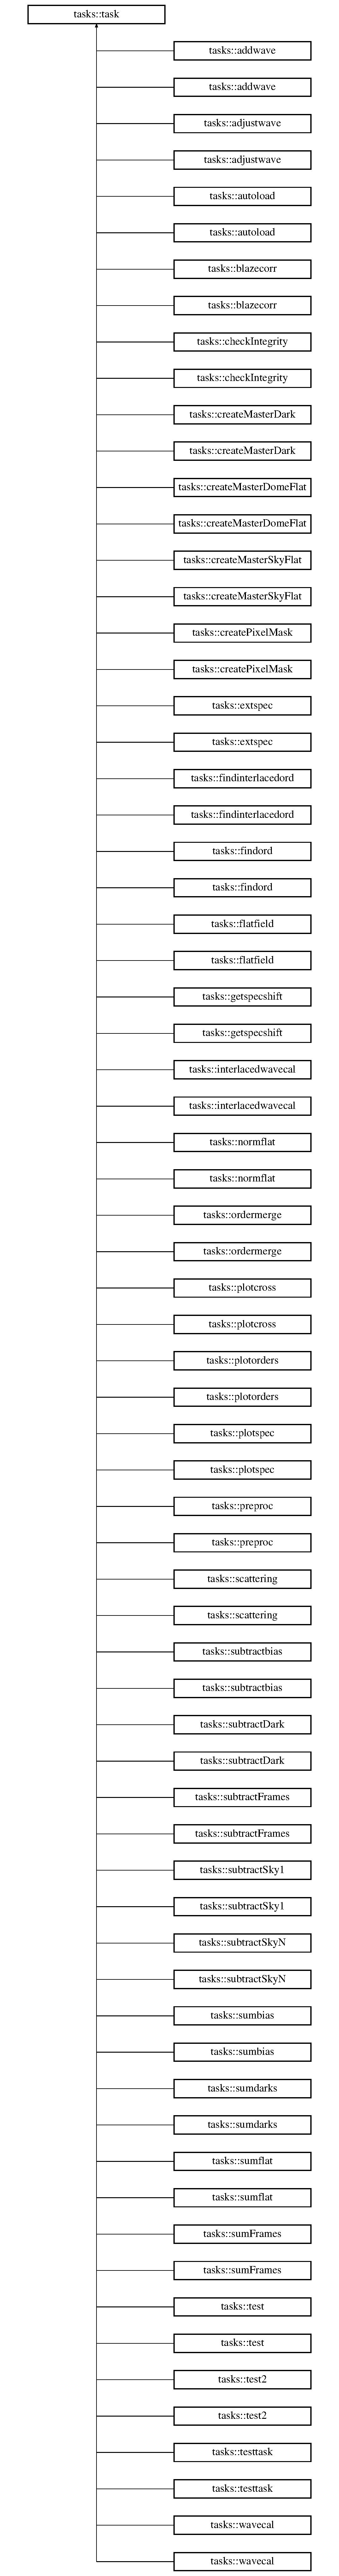
\includegraphics[height=12cm]{classtasks_1_1task}
\end{center}
\end{figure}
\subsection*{Public Member Functions}
\begin{CompactItemize}
\item 
def \textbf{\_\-\_\-init\_\-\_\-}\label{classtasks_1_1task_6c6d93968e1985dcdeb9a427e5887caf}

\item 
def \textbf{\_\-\_\-init\_\-\_\-}\label{classtasks_1_1task_6c6d93968e1985dcdeb9a427e5887caf}

\end{CompactItemize}
\subsection*{Static Public Attributes}
\begin{CompactItemize}
\item 
string \textbf{name} = 'undefined'\label{classtasks_1_1task_9d5daece96641b7ccc3b23b081699b6d}

\item 
string \textbf{button\-Text} = 'Not defined'\label{classtasks_1_1task_47c74a10937d34df8c3557b816f8f277}

\item 
\textbf{suffix} = None\label{classtasks_1_1task_6392c45806636706521d0d44d8bf9201}

\item 
int \textbf{inthread} = 1\label{classtasks_1_1task_a36a990ce7efee7b6e78f06c5b107675}

\item 
int \textbf{output} = 1\label{classtasks_1_1task_f090c423ef95574cf59a5349659a63cc}

\item 
list \textbf{prereq} = [$\,$]\label{classtasks_1_1task_224e6683b391e12fce9ff0882e5e012b}

\end{CompactItemize}


\subsection{Detailed Description}


\footnotesize\begin{verbatim}Description not given\end{verbatim}
\normalsize
 



The documentation for this class was generated from the following files:\begin{CompactItemize}
\item 
old/PANICtool-1.0/tasks.py\item 
old/tasks.py\end{CompactItemize}

\section{tasks::task\-Abort Class Reference}
\label{classtasks_1_1taskAbort}\index{tasks::taskAbort@{tasks::taskAbort}}
\subsection*{Public Member Functions}
\begin{CompactItemize}
\item 
def \textbf{\_\-\_\-init\_\-\_\-}\label{classtasks_1_1taskAbort_78ce6c70e9b2efac71ddf577426d37f5}

\item 
def \textbf{\_\-\_\-init\_\-\_\-}\label{classtasks_1_1taskAbort_78ce6c70e9b2efac71ddf577426d37f5}

\end{CompactItemize}
\subsection*{Public Attributes}
\begin{CompactItemize}
\item 
\textbf{args}\label{classtasks_1_1taskAbort_63920492ef729a7582a9d14293624dba}

\end{CompactItemize}


\subsection{Detailed Description}


\footnotesize\begin{verbatim}Module-specific error, to be raised when an the reduction is to be aborted
   in a friendly way. This error should be caught by the task manager, who
   then stops the processing.
\end{verbatim}
\normalsize
 



The documentation for this class was generated from the following files:\begin{CompactItemize}
\item 
old/PANICtool-1.0/tasks.py\item 
old/tasks.py\end{CompactItemize}

\section{tasks::task\-Error Class Reference}
\label{classtasks_1_1taskError}\index{tasks::taskError@{tasks::taskError}}
\subsection*{Public Member Functions}
\begin{CompactItemize}
\item 
def \textbf{\_\-\_\-init\_\-\_\-}\label{classtasks_1_1taskError_a072222b420274bbfb156e28a39df727}

\item 
def \textbf{\_\-\_\-init\_\-\_\-}\label{classtasks_1_1taskError_a072222b420274bbfb156e28a39df727}

\end{CompactItemize}
\subsection*{Public Attributes}
\begin{CompactItemize}
\item 
\textbf{args}\label{classtasks_1_1taskError_7d6e0cf7a415cd171699f9502995f90d}

\end{CompactItemize}


\subsection{Detailed Description}


\footnotesize\begin{verbatim}Module-specific error, to be raised when an 'expected' exception occurs
   during the processing of a task. This error should then be caught by the
   task manager, avoiding nasty error output.
\end{verbatim}
\normalsize
 



The documentation for this class was generated from the following files:\begin{CompactItemize}
\item 
old/PANICtool-1.0/tasks.py\item 
old/tasks.py\end{CompactItemize}

\section{reduce::threadsmod::Task\-Info Class Reference}
\label{classreduce_1_1threadsmod_1_1TaskInfo}\index{reduce::threadsmod::TaskInfo@{reduce::threadsmod::TaskInfo}}
\subsection*{Public Member Functions}
\begin{CompactItemize}
\item 
def \textbf{\_\-\_\-init\_\-\_\-}\label{classreduce_1_1threadsmod_1_1TaskInfo_f4e1c5c5065820c02fd213717712af6e}

\item 
def \textbf{clear}\label{classreduce_1_1threadsmod_1_1TaskInfo_a27e3183bf99a253c0eb9bdc70aa15d8}

\end{CompactItemize}


\subsection{Detailed Description}


\footnotesize\begin{verbatim}
Class where ExecTaskThread and WaitTaskThread share info and the result of execution
\end{verbatim}
\normalsize
 



The documentation for this class was generated from the following file:\begin{CompactItemize}
\item 
reduce/threadsmod.py\end{CompactItemize}

\section{configobj::Template\-Interpolation Class Reference}
\label{classconfigobj_1_1TemplateInterpolation}\index{configobj::TemplateInterpolation@{configobj::TemplateInterpolation}}
Inheritance diagram for configobj::Template\-Interpolation::\begin{figure}[H]
\begin{center}
\leavevmode
\includegraphics[height=2cm]{classconfigobj_1_1TemplateInterpolation}
\end{center}
\end{figure}


\subsection{Detailed Description}


\footnotesize\begin{verbatim}Behaves like string.Template.\end{verbatim}
\normalsize
 



The documentation for this class was generated from the following file:\begin{CompactItemize}
\item 
old/PANICtool-1.0/configobj.py\end{CompactItemize}

\section{tasks::test Class Reference}
\label{classtasks_1_1test}\index{tasks::test@{tasks::test}}
Inheritance diagram for tasks::test::\begin{figure}[H]
\begin{center}
\leavevmode
\includegraphics[height=2cm]{classtasks_1_1test}
\end{center}
\end{figure}
\subsection*{Public Member Functions}
\begin{CompactItemize}
\item 
def \textbf{\_\-\_\-init\_\-\_\-}\label{classtasks_1_1test_0cb323f022fd44123c950b76f061e776}

\item 
def \textbf{run}\label{classtasks_1_1test_798d0bc762bfddaef6de0058a4acf86f}

\item 
def \textbf{\_\-\_\-init\_\-\_\-}\label{classtasks_1_1test_0cb323f022fd44123c950b76f061e776}

\item 
def \textbf{run}\label{classtasks_1_1test_798d0bc762bfddaef6de0058a4acf86f}

\end{CompactItemize}
\subsection*{Static Public Attributes}
\begin{CompactItemize}
\item 
string \textbf{name} = '{\bftest}'\label{classtasks_1_1test_fedc868815b9ee3fcd3dde2b0acef22f}

\item 
string \textbf{button\-Text} = '{\bftest}'\label{classtasks_1_1test_d29763969e4128804e59324dee960c05}

\item 
int \textbf{inthread} = 0\label{classtasks_1_1test_d481510e691b04fbff713c2662a73c9e}

\end{CompactItemize}


\subsection{Detailed Description}


\footnotesize\begin{verbatim}Subtract two selected frames
\end{verbatim}
\normalsize
 



The documentation for this class was generated from the following files:\begin{CompactItemize}
\item 
old/PANICtool-1.0/tasks.py\item 
old/tasks.py\end{CompactItemize}

\section{tasks::test2 Class Reference}
\label{classtasks_1_1test2}\index{tasks::test2@{tasks::test2}}
Inheritance diagram for tasks::test2::\begin{figure}[H]
\begin{center}
\leavevmode
\includegraphics[height=2cm]{classtasks_1_1test2}
\end{center}
\end{figure}
\subsection*{Public Member Functions}
\begin{CompactItemize}
\item 
def \textbf{\_\-\_\-init\_\-\_\-}\label{classtasks_1_1test2_3471bd5d13ce9b406bbeaaf9ff95a276}

\item 
def \textbf{run}\label{classtasks_1_1test2_9c98ce5152399d4ff854b3da5c263354}

\item 
def \textbf{\_\-\_\-init\_\-\_\-}\label{classtasks_1_1test2_3471bd5d13ce9b406bbeaaf9ff95a276}

\item 
def \textbf{run}\label{classtasks_1_1test2_9c98ce5152399d4ff854b3da5c263354}

\end{CompactItemize}
\subsection*{Public Attributes}
\begin{CompactItemize}
\item 
\textbf{frame\_\-in}\label{classtasks_1_1test2_5f996eb068089f6bb0251020246959d8}

\item 
\textbf{frame\_\-out}\label{classtasks_1_1test2_cfdee3257fef1d67cf9c3c538abeb8ca}

\item 
\textbf{bd\-Pixel}\label{classtasks_1_1test2_16d25f922d1d5a3dc9ac52262cf2ccd1}

\end{CompactItemize}
\subsection*{Static Public Attributes}
\begin{CompactItemize}
\item 
string \textbf{name} = '{\bftest2}'\label{classtasks_1_1test2_6f30c5afb4d538f7046428a1112db228}

\item 
string \textbf{button\-Text} = '{\bftest2}'\label{classtasks_1_1test2_ff9a60ffbce17d2858d785d46fb37d64}

\end{CompactItemize}


\subsection{Detailed Description}


\footnotesize\begin{verbatim}
   A task only for tests
\end{verbatim}
\normalsize
 



The documentation for this class was generated from the following files:\begin{CompactItemize}
\item 
old/PANICtool-1.0/tasks.py\item 
old/tasks.py\end{CompactItemize}

\section{tasks::testtask Class Reference}
\label{classtasks_1_1testtask}\index{tasks::testtask@{tasks::testtask}}
Inheritance diagram for tasks::testtask::\begin{figure}[H]
\begin{center}
\leavevmode
\includegraphics[height=2cm]{classtasks_1_1testtask}
\end{center}
\end{figure}
\subsection*{Public Member Functions}
\begin{CompactItemize}
\item 
def \textbf{run}\label{classtasks_1_1testtask_00fe50b803e43fde0d25bfc73aa436c1}

\item 
def \textbf{run}\label{classtasks_1_1testtask_00fe50b803e43fde0d25bfc73aa436c1}

\end{CompactItemize}
\subsection*{Static Public Attributes}
\begin{CompactItemize}
\item 
string \textbf{name} = 'skeleton'\label{classtasks_1_1testtask_8f077e1e4f67469fa5cf6e0c22a02997}

\item 
string \textbf{button\-Text} = 'Does really nothing!'\label{classtasks_1_1testtask_53905d7258165161f7a752124a7e4aba}

\end{CompactItemize}


\subsection{Detailed Description}


\footnotesize\begin{verbatim}
   This task does nothing (except for writing to the log file). The help text
   that should appear in the interface should go here
\end{verbatim}
\normalsize
 



The documentation for this class was generated from the following files:\begin{CompactItemize}
\item 
old/PANICtool-1.0/tasks.py\item 
old/tasks.py\end{CompactItemize}

\section{configobj::Unrepr\-Error Class Reference}
\label{classconfigobj_1_1UnreprError}\index{configobj::UnreprError@{configobj::UnreprError}}
Inheritance diagram for configobj::Unrepr\-Error::\begin{figure}[H]
\begin{center}
\leavevmode
\includegraphics[height=2cm]{classconfigobj_1_1UnreprError}
\end{center}
\end{figure}


\subsection{Detailed Description}


\footnotesize\begin{verbatim}An error parsing in unrepr mode.\end{verbatim}
\normalsize
 



The documentation for this class was generated from the following file:\begin{CompactItemize}
\item 
old/PANICtool-1.0/configobj.py\end{CompactItemize}

\section{auto\-Loader::User\-Dict Class Reference}
\label{classautoLoader_1_1UserDict}\index{autoLoader::UserDict@{autoLoader::UserDict}}
\subsection*{Public Member Functions}
\begin{CompactItemize}
\item 
def \textbf{\_\-\_\-init\_\-\_\-}\label{classautoLoader_1_1UserDict_f3479a330743164ac42c0614ad3d7fdb}

\item 
def \textbf{\_\-\_\-repr\_\-\_\-}\label{classautoLoader_1_1UserDict_bfe58f769f3a894978c693f40c944cec}

\item 
def \textbf{\_\-\_\-cmp\_\-\_\-}\label{classautoLoader_1_1UserDict_d3d690836033a91d2d001ed908c4790a}

\item 
def \textbf{\_\-\_\-len\_\-\_\-}\label{classautoLoader_1_1UserDict_90bcd535e7934a7d34d1432734eabfd4}

\item 
def \textbf{\_\-\_\-getitem\_\-\_\-}\label{classautoLoader_1_1UserDict_d035a626230ba56912779427ec634eb7}

\item 
def \textbf{\_\-\_\-setitem\_\-\_\-}\label{classautoLoader_1_1UserDict_7e55cb7c77a92f25bf6134d85981ad23}

\item 
def \textbf{\_\-\_\-delitem\_\-\_\-}\label{classautoLoader_1_1UserDict_d75da32f9d0480eec739c527c285ffaf}

\item 
def \textbf{keys}\label{classautoLoader_1_1UserDict_a86511e267a538229efc85f3a454fe6a}

\item 
def \textbf{items}\label{classautoLoader_1_1UserDict_452b092fba0b7508d4abac71ff1a4939}

\item 
def \textbf{values}\label{classautoLoader_1_1UserDict_98fa26c41c1d55c6d06ed2df222a525c}

\item 
def \textbf{has\_\-key}\label{classautoLoader_1_1UserDict_b8f1844abe33a10d7c6e99b83d6f4133}

\end{CompactItemize}
\subsection*{Public Attributes}
\begin{CompactItemize}
\item 
\textbf{data}\label{classautoLoader_1_1UserDict_a3ce6477de9edf79bdd6cf247037499c}

\end{CompactItemize}


\subsection{Detailed Description}


\footnotesize\begin{verbatim}
   Custom class mimicing the behavior of a dictionary object.
   This class in necessary because inheriting methods from the dictionary
   object does not give all the needed functionality, and no further object
   can be attached.
\end{verbatim}
\normalsize
 



The documentation for this class was generated from the following file:\begin{CompactItemize}
\item 
old/PANICtool-1.0/auto\-Loader.py\end{CompactItemize}

\section{reduce::threadsmod::Wait\-Task\-Thread Class Reference}
\label{classreduce_1_1threadsmod_1_1WaitTaskThread}\index{reduce::threadsmod::WaitTaskThread@{reduce::threadsmod::WaitTaskThread}}
\subsection*{Public Member Functions}
\begin{CompactItemize}
\item 
def \textbf{\_\-\_\-init\_\-\_\-}\label{classreduce_1_1threadsmod_1_1WaitTaskThread_f644ca33ce0f909b9c712be9bbc66f99}

\item 
def \textbf{run}\label{classreduce_1_1threadsmod_1_1WaitTaskThread_1957bc7b47b8ae618751318bd4d5a824}

\end{CompactItemize}


\subsection{Detailed Description}


\footnotesize\begin{verbatim}
NOT USED until now
NOT USED until now
NOT USED until now

Thread waiting for a task until a signal event is received

NOT USED until now
NOT USED until now
NOT USED until now

\end{verbatim}
\normalsize
 



The documentation for this class was generated from the following file:\begin{CompactItemize}
\item 
reduce/threadsmod.py\end{CompactItemize}

\section{tasks::wavecal Class Reference}
\label{classtasks_1_1wavecal}\index{tasks::wavecal@{tasks::wavecal}}
Inheritance diagram for tasks::wavecal::\begin{figure}[H]
\begin{center}
\leavevmode
\includegraphics[height=2cm]{classtasks_1_1wavecal}
\end{center}
\end{figure}
\subsection*{Public Member Functions}
\begin{CompactItemize}
\item 
def \textbf{run}\label{classtasks_1_1wavecal_f6be9eb15626e914a716d2cea7dd733a}

\item 
def \textbf{run}\label{classtasks_1_1wavecal_f6be9eb15626e914a716d2cea7dd733a}

\end{CompactItemize}
\subsection*{Static Public Attributes}
\begin{CompactItemize}
\item 
string \textbf{name} = '{\bfwavecal}'\label{classtasks_1_1wavecal_662466b5dca4887cf29a1544ff540e4e}

\item 
string \textbf{button\-Text} = 'Find wavelength solution'\label{classtasks_1_1wavecal_8d305b5a22837dda6b63b083284d3403}

\item 
list \textbf{prereq} = ['{\bffindord}']\label{classtasks_1_1wavecal_00ba057428243ec2132a86836fe0ad1b}

\item 
int \textbf{inthread} = 0\label{classtasks_1_1wavecal_be011617a0ed60b4abde6e02f292027a}

\end{CompactItemize}


\subsection{Detailed Description}


\footnotesize\begin{verbatim}Interactively determine a 2-dimensional wavelength definition from a
   well-exposed wavelength definition frame, normally an ThAr frame.
\end{verbatim}
\normalsize
 



The documentation for this class was generated from the following files:\begin{CompactItemize}
\item 
old/PANICtool-1.0/tasks.py\item 
old/tasks.py\end{CompactItemize}

\section{plot\-Frame::window Class Reference}
\label{classplotFrame_1_1window}\index{plotFrame::window@{plotFrame::window}}
\subsection*{Public Member Functions}
\begin{CompactItemize}
\item 
def \textbf{\_\-\_\-init\_\-\_\-}\label{classplotFrame_1_1window_cfaf753aae848029420c85559bde6251}

\item 
def \textbf{make\-Frame}\label{classplotFrame_1_1window_35d25d026b0d2a5876d569214fee02ab}

\item 
def {\bfplot\-Spec}
\item 
def \textbf{print\-Spec}\label{classplotFrame_1_1window_929ce03e4282b70d4d99bc4b688a8cc3}

\end{CompactItemize}
\subsection*{Public Attributes}
\begin{CompactItemize}
\item 
\textbf{lastplotname}\label{classplotFrame_1_1window_dc31634cec52cdb0487ccd5910e247d3}

\item 
\textbf{usebiggles}\label{classplotFrame_1_1window_2f73eb744ee20ec837b63ca26698c49b}

\item 
\textbf{root}\label{classplotFrame_1_1window_ce5b00741bbdb3736f69c3242f8acb9c}

\end{CompactItemize}


\subsection{Detailed Description}


\footnotesize\begin{verbatim}
   Provide a window to manage the automatic or manual plotting of spectra. The
   user is able to provide axis boundaries, and can choose to use the
   quicklook plotting program 'Biggles', or the more extended IRAF interface.
\end{verbatim}
\normalsize
 



\subsection{Member Function Documentation}
\index{plotFrame::window@{plot\-Frame::window}!plotSpec@{plotSpec}}
\index{plotSpec@{plotSpec}!plotFrame::window@{plot\-Frame::window}}
\subsubsection{\setlength{\rightskip}{0pt plus 5cm}def plot\-Frame::window::plot\-Spec ( {\em self},  {\em filename} = {\tt None},  {\em plotother} = {\tt False})}\label{classplotFrame_1_1window_869b6a593553ce9895e4c5ca468b4782}




\footnotesize\begin{verbatim}
   Determine the current state of the widget entries and plot the
   spectrum accordingly.
\end{verbatim}
\normalsize
 

The documentation for this class was generated from the following file:\begin{CompactItemize}
\item 
old/PANICtool-1.0/plot\-Frame.py\end{CompactItemize}

\section{engin\-Frame::window Class Reference}
\label{classenginFrame_1_1window}\index{enginFrame::window@{enginFrame::window}}
\subsection*{Public Member Functions}
\begin{CompactItemize}
\item 
def \textbf{\_\-\_\-init\_\-\_\-}\label{classenginFrame_1_1window_dff1502cf3315e4d696da726ef5ff9c4}

\item 
def \textbf{make\-Frame}\label{classenginFrame_1_1window_dcfb7d7047f7d4974ec2c859c4ec4193}

\item 
def \textbf{show}\label{classenginFrame_1_1window_7144f17c367253a628d99e29c6743621}

\item 
def \textbf{hide}\label{classenginFrame_1_1window_1244e0a4dcf3db9c027ccbb5091d852d}

\item 
def \textbf{update}\label{classenginFrame_1_1window_974988f74537467a0e064f7495f4e86c}

\item 
def \textbf{disable}\label{classenginFrame_1_1window_e817a5f913a27ff75d20b5c456104561}

\item 
def \textbf{enable}\label{classenginFrame_1_1window_026f8b0d8d1e6c1035faf7b9e215f0b1}

\item 
def \textbf{run\-Task}\label{classenginFrame_1_1window_a3da27cfd404abe2f584a74bf6c7afe7}

\end{CompactItemize}
\subsection*{Public Attributes}
\begin{CompactItemize}
\item 
\textbf{parent}\label{classenginFrame_1_1window_eef677aa71694ca3b693524d6025dc44}

\item 
\textbf{GUIupdater}\label{classenginFrame_1_1window_836fd2e0ffe696063bd80cdd6d9f2665}

\item 
\textbf{currentmode}\label{classenginFrame_1_1window_ce0958eee7f8172b06b577546f37918c}

\item 
\textbf{top}\label{classenginFrame_1_1window_5d56f21afe0d103e777d9b2f8a7c5bc0}

\item 
\textbf{canvas}\label{classenginFrame_1_1window_f648108fa82f2a365bc431f495772bdd}

\item 
\textbf{taskbars}\label{classenginFrame_1_1window_c3dd027c632c7bbd187a746a69fd6fe2}

\item 
\textbf{root}\label{classenginFrame_1_1window_ba00a841b0f1cba909d7fa63cc95d3db}

\item 
\textbf{tasklist}\label{classenginFrame_1_1window_4cc5b86f0ff1828c73a58bf555ee8300}

\item 
\textbf{button1}\label{classenginFrame_1_1window_e57cfbda5d1d48209a26e6cb66c2dd43}

\item 
\textbf{okbutton}\label{classenginFrame_1_1window_a8994c844c6ccbd687e16720aebff99a}

\end{CompactItemize}


\subsection{Detailed Description}


\footnotesize\begin{verbatim}
   Provide a window to execute the calibration tasks, and set essential
   parameters, such as the location of input and output calibration frames.
   Class inherits from Tkinter's 'Frame' class.
\end{verbatim}
\normalsize
 



The documentation for this class was generated from the following file:\begin{CompactItemize}
\item 
old/PANICtool-1.0/engin\-Frame.py\end{CompactItemize}

\section{pipe\-Frame::window Class Reference}
\label{classpipeFrame_1_1window}\index{pipeFrame::window@{pipeFrame::window}}
\subsection*{Public Member Functions}
\begin{CompactItemize}
\item 
def \textbf{\_\-\_\-init\_\-\_\-}\label{classpipeFrame_1_1window_13e65fc7ab9193f5bc329da08fcd4c60}

\item 
def \textbf{make\-Frame}\label{classpipeFrame_1_1window_861837594f13db6d2eb3442e6d01f1c1}

\item 
def \textbf{disable}\label{classpipeFrame_1_1window_0b36dfff8fe441034c614aaf8208c226}

\item 
def \textbf{enable}\label{classpipeFrame_1_1window_cec1cff7cd9347d559af418ea689dc96}

\item 
def \textbf{clear}\label{classpipeFrame_1_1window_92aa6dd93c83f76e31d97c2201b9317e}

\item 
def \textbf{reset}\label{classpipeFrame_1_1window_21a7918f8f1f72c19a82f16af2d65a03}

\item 
def {\bfprocess\_\-frame}
\item 
def \textbf{run\_\-pipe}\label{classpipeFrame_1_1window_d5ac12b11714aecdd31527ab8edbef25}

\end{CompactItemize}
\subsection*{Public Attributes}
\begin{CompactItemize}
\item 
\textbf{parent}\label{classpipeFrame_1_1window_161bdbc1c1dc5ae2b6b27bcbd93b885d}

\item 
\textbf{GUIupdater}\label{classpipeFrame_1_1window_2aa7161a56d0e64c028215f917cfa1b8}

\item 
\textbf{defaultbgcolor}\label{classpipeFrame_1_1window_33936e413678af26fe2bc8d153b34b6a}

\item 
\textbf{selectedtasks}\label{classpipeFrame_1_1window_a759eb2b6a71d53a47045e0c80e75693}

\item 
\textbf{taskbars}\label{classpipeFrame_1_1window_f87d0234b3e716908dad1c4d2fad26c6}

\item 
\textbf{tasklist}\label{classpipeFrame_1_1window_080698195d4902157a0ff9d91127029a}

\item 
\textbf{mode}\label{classpipeFrame_1_1window_e0f9c9e281da8f639b5cc8103e2a4489}

\item 
\textbf{out\-Queue}\label{classpipeFrame_1_1window_3767f9a1c1efc5578b243901b01114b9}

\item 
\textbf{root}\label{classpipeFrame_1_1window_b4c8077063c841e4a827b1911ca5ea15}

\item 
\textbf{currentmode}\label{classpipeFrame_1_1window_2aab046093bff1e9b9d73135fca3b638}

\end{CompactItemize}


\subsection{Detailed Description}


\footnotesize\begin{verbatim}
   Provide a frame displaying the tasks that are to be executed for the
   current reduction mode defined in 'self.mode'.
\end{verbatim}
\normalsize
 



\subsection{Member Function Documentation}
\index{pipeFrame::window@{pipe\-Frame::window}!process_frame@{process\_\-frame}}
\index{process_frame@{process\_\-frame}!pipeFrame::window@{pipe\-Frame::window}}
\subsubsection{\setlength{\rightskip}{0pt plus 5cm}def pipe\-Frame::window::process\_\-frame ( {\em self},  {\em frame})}\label{classpipeFrame_1_1window_d96488cdd2d7089356199d602813f5dd}




\footnotesize\begin{verbatim}
   Prepare a child thread to do the reduction of a single frame. (Will
   run in main thread)
\end{verbatim}
\normalsize
 

The documentation for this class was generated from the following file:\begin{CompactItemize}
\item 
old/PANICtool-1.0/pipe\-Frame.py\end{CompactItemize}

\section{auto\-Queue::window Class Reference}
\label{classautoQueue_1_1window}\index{autoQueue::window@{autoQueue::window}}
\subsection*{Public Member Functions}
\begin{CompactItemize}
\item 
def \textbf{\_\-\_\-init\_\-\_\-}\label{classautoQueue_1_1window_f9b1f2279170e293ec3be13e7ec29fca}

\item 
def \textbf{make\-Frame}\label{classautoQueue_1_1window_2129bd61518872f8b89930b33d39aa4a}

\item 
def \textbf{update\-Queue\-Size}\label{classautoQueue_1_1window_4c08934dfe0535b02e6eb8699def7fe2}

\item 
def {\bfauto\-Check\-Files}
\item 
def {\bffind\-New\-Files}
\item 
def \textbf{edit\-New\-Files}\label{classautoQueue_1_1window_41e66e3250f7a972569530201417cca8}

\item 
def \textbf{edit\-Reduced\-Files}\label{classautoQueue_1_1window_c368f76941f17394f7fdd649b48e5611}

\end{CompactItemize}
\subsection*{Public Attributes}
\begin{CompactItemize}
\item 
\textbf{filterpattern}\label{classautoQueue_1_1window_2c6966db2ae8251f70d9c1c8c7673d44}

\item 
\textbf{queuesize}\label{classautoQueue_1_1window_782e915f368466d2520ca4bde42d55c7}

\item 
\textbf{reducedsize}\label{classautoQueue_1_1window_e053e1e70de057a0be4c4869d0eec810}

\item 
\textbf{autocheck}\label{classautoQueue_1_1window_98b87f8b2d8858d814f75d8450c6e72b}

\item 
\textbf{newfiles}\label{classautoQueue_1_1window_9d59335fec278298ad6bbc6ab8eadbf7}

\item 
\textbf{reducedfiles}\label{classautoQueue_1_1window_ef6f941e2752b7104cb3b2b9d49e3c35}

\item 
\textbf{check\-ID}\label{classautoQueue_1_1window_95334378a838a39f3a5b9e0c5d31469c}

\item 
\textbf{root}\label{classautoQueue_1_1window_c9a07eca0e452cc5dc853daf0977de26}

\end{CompactItemize}


\subsection{Detailed Description}


\footnotesize\begin{verbatim}
   Provides a window to manage the unprocessed and processed queues, as
   well as methods to automatically update these queues. Class inherits
   from Tkinter's 'Frame' class.
\end{verbatim}
\normalsize
 



\subsection{Member Function Documentation}
\index{autoQueue::window@{auto\-Queue::window}!autoCheckFiles@{autoCheckFiles}}
\index{autoCheckFiles@{autoCheckFiles}!autoQueue::window@{auto\-Queue::window}}
\subsubsection{\setlength{\rightskip}{0pt plus 5cm}def auto\-Queue::window::auto\-Check\-Files ( {\em self})}\label{classautoQueue_1_1window_8753071d1a4953ca0a0bdc78c9a2b3f3}




\footnotesize\begin{verbatim}
   Invoked when the autocheck checkbox is toggled. Depending upon whether
   it was selected or deselected, will start or stop the automatic
   checking for new files for the unprocessed queue.
\end{verbatim}
\normalsize
 \index{autoQueue::window@{auto\-Queue::window}!findNewFiles@{findNewFiles}}
\index{findNewFiles@{findNewFiles}!autoQueue::window@{auto\-Queue::window}}
\subsubsection{\setlength{\rightskip}{0pt plus 5cm}def auto\-Queue::window::find\-New\-Files ( {\em self})}\label{classautoQueue_1_1window_be4ca93befd0bd2e2805c61f8143c6d7}




\footnotesize\begin{verbatim}
   Find files that are not yet listed in the queue of unprocessed
   files, and match these with the filename filter pattern
\end{verbatim}
\normalsize
 

The documentation for this class was generated from the following file:\begin{CompactItemize}
\item 
old/PANICtool-1.0/auto\-Queue.py\end{CompactItemize}

\section{config\-Frame::window Class Reference}
\label{classconfigFrame_1_1window}\index{configFrame::window@{configFrame::window}}
\subsection*{Public Member Functions}
\begin{CompactItemize}
\item 
def \textbf{\_\-\_\-init\_\-\_\-}\label{classconfigFrame_1_1window_732edf380f9105604d18ff185c3f8ce0}

\item 
def \textbf{make\-Frame}\label{classconfigFrame_1_1window_37671e7e33f66fbd67278ba61b070726}

\item 
def {\bfshow}
\item 
def \textbf{hide}\label{classconfigFrame_1_1window_b5365cf3ea2ee9f7801b11221e01a999}

\item 
def \textbf{update}\label{classconfigFrame_1_1window_633d5287d7edcee37b5482b7556c682f}

\item 
def \textbf{autoupdate}\label{classconfigFrame_1_1window_f87dc2a4622331c88c9c6ef38d6bed78}

\item 
def \textbf{save\-Config}\label{classconfigFrame_1_1window_e466f40928ac9070f07f192b3a77b1e2}

\item 
def \textbf{load\-Config}\label{classconfigFrame_1_1window_dacd305584989dc39a67990c6d5c1dee}

\item 
def \textbf{reset\-Config}\label{classconfigFrame_1_1window_07db147a114ea9eb08e2a398c80ab420}

\end{CompactItemize}
\subsection*{Public Attributes}
\begin{CompactItemize}
\item 
\textbf{title}\label{classconfigFrame_1_1window_818ffaa4f584e5703371df4e4899d746}

\item 
\textbf{embed}\label{classconfigFrame_1_1window_38119dcbec5148e3e1ac4c70f8356071}

\item 
\textbf{minwidth}\label{classconfigFrame_1_1window_60ba76187ff08eb4d6a003be6eea7bda}

\item 
\textbf{top}\label{classconfigFrame_1_1window_df66ebeada4f6f4e77f4babbcbf7c293}

\item 
\textbf{canvas}\label{classconfigFrame_1_1window_f0d47b9dc39b396a0c863c1c8204e5b5}

\item 
\textbf{optionlist}\label{classconfigFrame_1_1window_189c7502b4fec783ee6bb92c4bea60a6}

\item 
\textbf{oldoptions}\label{classconfigFrame_1_1window_91109bfb6bc432ae55ec42e9a32687a2}

\item 
\textbf{root}\label{classconfigFrame_1_1window_9280084b54466b46d28b5df01579dd68}

\item 
\textbf{optionbuttonlist}\label{classconfigFrame_1_1window_80aae05fd345bcbd5fe80afc0aa2c2c4}

\end{CompactItemize}


\subsection{Detailed Description}


\footnotesize\begin{verbatim}
   Provide a window to edit settings defined in the 'config' module
\end{verbatim}
\normalsize
 



\subsection{Member Function Documentation}
\index{configFrame::window@{config\-Frame::window}!show@{show}}
\index{show@{show}!configFrame::window@{config\-Frame::window}}
\subsubsection{\setlength{\rightskip}{0pt plus 5cm}def config\-Frame::window::show ( {\em self})}\label{classconfigFrame_1_1window_7b5e7f961d3544457f6d7d9f2d2c69b7}




\footnotesize\begin{verbatim}
   If embedded, display this window. If top-level, then deiconify and set
   focus and grab to this window
\end{verbatim}
\normalsize
 

The documentation for this class was generated from the following file:\begin{CompactItemize}
\item 
old/PANICtool-1.0/config\-Frame.py\end{CompactItemize}

\section{auto\-Loader::window Class Reference}
\label{classautoLoader_1_1window}\index{autoLoader::window@{autoLoader::window}}
\subsection*{Public Member Functions}
\begin{CompactItemize}
\item 
def {\bf\_\-\_\-init\_\-\_\-}
\item 
def \textbf{make\-Frame}\label{classautoLoader_1_1window_3118bba3001fcb0b270a1c3d2a29a6bb}

\item 
def \textbf{show}\label{classautoLoader_1_1window_1ffbf23a2106138a9f6144460aeb5bbf}

\item 
def \textbf{hide}\label{classautoLoader_1_1window_fbb1e5df3f8eea618a22d80f077e5288}

\item 
def {\bfreadentries}
\item 
def {\bfwriteentries}
\item 
def \textbf{reset}\label{classautoLoader_1_1window_ebd2bb75453b65cf2c5c627893f81f9a}

\item 
def {\bftest\-Rule\-Set}
\item 
def \textbf{del\-Rule}\label{classautoLoader_1_1window_7d6be5c803fa09e4f77b0530320cbe29}

\item 
def \textbf{add\-Rule}\label{classautoLoader_1_1window_1a222201b5a73af6a0447cbbb5cf8e03}

\item 
def \textbf{pick\-File}\label{classautoLoader_1_1window_e5678fcb23c6cfb13079d0dcab545654}

\item 
def \textbf{save\-Config}\label{classautoLoader_1_1window_ac7f28121ad44fea4ae78c97ea7d0c15}

\item 
def \textbf{load\-Config}\label{classautoLoader_1_1window_10cd0a27f8527999abf07747c7baf0cf}

\end{CompactItemize}
\subsection*{Public Attributes}
\begin{CompactItemize}
\item 
\textbf{topframe}\label{classautoLoader_1_1window_ed443f71b4f4ade6f64cea9f1ce46117}

\end{CompactItemize}


\subsection{Detailed Description}


\footnotesize\begin{verbatim}
   Construct a window to modify and test a set of autoLoading rules
\end{verbatim}
\normalsize
 



\subsection{Member Function Documentation}
\index{autoLoader::window@{auto\-Loader::window}!__init__@{\_\-\_\-init\_\-\_\-}}
\index{__init__@{\_\-\_\-init\_\-\_\-}!autoLoader::window@{auto\-Loader::window}}
\subsubsection{\setlength{\rightskip}{0pt plus 5cm}def auto\-Loader::window::\_\-\_\-init\_\-\_\- ( {\em self},  {\em parent},  {\em title} = {\tt 'Configuration~for~autoloading~configuration~files'})}\label{classautoLoader_1_1window_be05368f9b50de9a67dbaa6b8a668263}




\footnotesize\begin{verbatim}
   Define the initial ruleset (if given in configuration) and create the
   rule editing frame
\end{verbatim}
\normalsize
 \index{autoLoader::window@{auto\-Loader::window}!readentries@{readentries}}
\index{readentries@{readentries}!autoLoader::window@{auto\-Loader::window}}
\subsubsection{\setlength{\rightskip}{0pt plus 5cm}def auto\-Loader::window::readentries ( {\em self})}\label{classautoLoader_1_1window_b05cd8b1b0902a674b9976d04673959a}




\footnotesize\begin{verbatim}
   Read the values that are currently in the widget, and store these values
   in the ruleset. Copy the existing ruleset to the system configuration
   object.
\end{verbatim}
\normalsize
 \index{autoLoader::window@{auto\-Loader::window}!writeentries@{writeentries}}
\index{writeentries@{writeentries}!autoLoader::window@{auto\-Loader::window}}
\subsubsection{\setlength{\rightskip}{0pt plus 5cm}def auto\-Loader::window::writeentries ( {\em self})}\label{classautoLoader_1_1window_78a8f457e9da084ff07da3f804395d70}




\footnotesize\begin{verbatim}
   Take the values of the ruleset object and write these to the widget
   elements on the screen
\end{verbatim}
\normalsize
 \index{autoLoader::window@{auto\-Loader::window}!testRuleSet@{testRuleSet}}
\index{testRuleSet@{testRuleSet}!autoLoader::window@{auto\-Loader::window}}
\subsubsection{\setlength{\rightskip}{0pt plus 5cm}def auto\-Loader::window::test\-Rule\-Set ( {\em self})}\label{classautoLoader_1_1window_db7269382b63a9072dcda500e6013ec1}




\footnotesize\begin{verbatim}
   Let the user select a FITS file to which the ruleset will be applied.
   Results are shown in a popup window.
\end{verbatim}
\normalsize
 

The documentation for this class was generated from the following file:\begin{CompactItemize}
\item 
old/PANICtool-1.0/auto\-Loader.py\end{CompactItemize}

\section{calib\-Frame::window Class Reference}
\label{classcalibFrame_1_1window}\index{calibFrame::window@{calibFrame::window}}
\subsection*{Public Member Functions}
\begin{CompactItemize}
\item 
def \textbf{\_\-\_\-init\_\-\_\-}\label{classcalibFrame_1_1window_d5e04d18d63d09e321190139ef0a7bc0}

\item 
def \textbf{make\-Frame}\label{classcalibFrame_1_1window_97e4321c21bad9765f2a9b4c1dd21ec5}

\item 
def \textbf{show}\label{classcalibFrame_1_1window_4e8ee7734b1901de09d408953ee4831c}

\item 
def \textbf{hide}\label{classcalibFrame_1_1window_358c2cb4c37e990480378ecf282c170f}

\item 
def \textbf{update}\label{classcalibFrame_1_1window_6d58b223b8fd49b226baf35b3381ffbb}

\item 
def \textbf{disable}\label{classcalibFrame_1_1window_255027b51999d6a08b3d44a2cb3d141e}

\item 
def \textbf{enable}\label{classcalibFrame_1_1window_8610595111d5e62dae720a29c93c22f3}

\item 
def \textbf{run\-Task}\label{classcalibFrame_1_1window_f36f4b2354a64c5deda47446fc9db4c0}

\end{CompactItemize}
\subsection*{Public Attributes}
\begin{CompactItemize}
\item 
\textbf{parent}\label{classcalibFrame_1_1window_c64247a7e8b90f7764680240f50cb4c7}

\item 
\textbf{GUIupdater}\label{classcalibFrame_1_1window_7f9296ebe6da5230ab7b4de296428370}

\item 
\textbf{currentmode}\label{classcalibFrame_1_1window_663fd2c07f8b2dc2a6a645cc843bbd67}

\item 
\textbf{top}\label{classcalibFrame_1_1window_3b56e2c64bb8977dc7a589574a6389d7}

\item 
\textbf{canvas}\label{classcalibFrame_1_1window_e345e475f537a04b88cfe3fd7e74fd37}

\item 
\textbf{taskbars}\label{classcalibFrame_1_1window_8f422bd67539d5dd05a4ccf6b2730e6f}

\item 
\textbf{root}\label{classcalibFrame_1_1window_98b27aa8b89dee2381d31e2d4e602745}

\item 
\textbf{tasklist}\label{classcalibFrame_1_1window_12d912bad2e3542c6d8845408904e639}

\item 
\textbf{okbutton}\label{classcalibFrame_1_1window_59212a8b98a820ef63c92bb8aa49d533}

\end{CompactItemize}


\subsection{Detailed Description}


\footnotesize\begin{verbatim}
   Provide a window to execute the calibration tasks, and set essential
   parameters, such as the location of input and output calibration frames.
   Class inherits from Tkinter's 'Frame' class.
\end{verbatim}
\normalsize
 



The documentation for this class was generated from the following file:\begin{CompactItemize}
\item 
old/PANICtool-1.0/calib\-Frame.py\end{CompactItemize}

\printindex
\end{document}
